\documentclass[11pt]{article}
\usepackage[margin=1in]{geometry}
\usepackage{amsmath,amssymb,amsthm,mathtools}
\usepackage{longtable}
\usepackage{booktabs,enumitem,graphicx,xcolor}
\usepackage{xurl}
\usepackage[section]{placeins}
\usepackage[colorlinks=true,linkcolor=blue!50!black,citecolor=green!35!black,urlcolor=blue!50!black]{hyperref}
\usepackage[nameinlink]{cleveref}
\newtheorem{theorem}{Theorem}\renewcommand{\thetheorem}{\Alph{theorem}}
\newtheorem{proposition}{Proposition}\newtheorem{corollary}{Corollary}\newtheorem{lemma}{Lemma}
\theoremstyle{definition}\newtheorem{definition}{Definition}\newtheorem{remark}{Remark}
\newcommand{\R}{\mathbb R}
\setlength{\emergencystretch}{3em}
\title{A Lab for Latent Actors:\\ Hiding Segments, Probes, Settled Decisions, Injected Records and Sources}
\author{Vinay K Awasthi\\ Johns Hopkins University\\ \texttt{vawasth1@jh.edu}}
\date{October 2026}
\begin{document}
\maketitle

\begin{abstract}
Two kinds of patient, invisible in the data, can explain every trial result. The first question is which part of their structure the
evidence actually reveals. The second is how a decision maker can force the rest into view, especially when someone with an interest
in the outcome chooses what is revealed. This companion to the note \emph{Partial Gluing and Level Two} \cite{PG} builds a
synthetic laboratory for these questions. It is run as an observe--orient--decide--act loop. Part I proves four theorems.
\begin{itemize}
\item \emph{Theorem A (hiding segment).} Pair tables never identify two latent types. They leave a segment of explanations, on which
  the probability of every event on $k$ variables is a polynomial of degree at most $k-2$ in one unseen parameter. A small subgroup that
  is very different is indistinguishable from a large one that is mildly different.
\item \emph{Theorem B (tempo).} Under pair-only disclosure the weight is never learned (tempo zero). After one informative triple
  table everything converges at $n^{-1/2}$. Agreement on a single variable is a regular relation. Only the merge of the two types
  slows to $n^{-1/4}$.
\item \emph{Theorem C (stratified value of information).} A probe is worthless when it touches a variable on which the types agree, and
  collapses the segment otherwise. Its worst-case value is zero whenever the decision has a saddle point on the segment, as a
  treat-or-not choice does, while its minimax-regret value stays positive whenever the best act changes. Its graded value rises with an explicit signal, and the best probe can be named from the pair
  tables alone. With verifiable disclosure and a skeptical regulator, sponsors unravel. A robust decision maker can lose from new
  evidence only when that evidence makes the evidence as a whole vacuous.
\item \emph{Theorem D (the decision on the segment).} An act is safe on the whole segment iff it is safe at both walls, and the
  set-rule choice depends on the pair tables alone, so no undetectable perturbation changes it. Info-gap prefers acts least exposed to
  the hidden moment, but before the probe its nominal point is a convention. After a probe the decision settles on the oracle act at
  median sample size $n^*=(z\tau/d)^2$, where $d$ is a computable radius, and never settles when the truth sits on a boundary.
  In the ring of contingency tables the worst case is a tropical limit of the table count rather than a section, $n^*$ is not a
  wall-crossing, and the exact conditional probe on the fibre is the efficient one (\cref{sec:ehrhart}).
\end{itemize}
Part II turns to an actor who adds records to tilt the decision, with no relation between injected and genuine records.
\begin{itemize}
\item \emph{Theorem E (slopes).} A decision's margin has a price in injected records: the margin divided by the steepest single-record
  influence, attained by copies of one record.
\item \emph{Theorem F (the hidden channel).} Injections that leave every pair table unchanged form a segment of their own. They move the
  estimate of the unseen parameter by $\varepsilon s/v_T$ while the regulator's segment stays put, so there is always a window in which
  the decision is taken over and nothing is flagged. The best probe is also the hardest to poison.
\item \emph{Theorem G (stealth with equations).} With four variables the tetrads can detect injection, except along their tangent
  directions. Those directions multiply on the strata, but there the André--Quillen obstruction stops them from being extended.
\item \emph{Theorem H (one geometry).} The adversary's segment and the regulator's are the positivity part and the model part of one
  line, read in units of $v_T$. The regulator's margin is the distance to the decision boundary and the adversary's room the distance
  to the detection boundary, so Part II completes the decision lab rather than adding to it.
\item \emph{Theorem J (sources and bands).} When the decision maker sees which source and batch each table came from, a trusted source
  that is adversarial in some batches can move the pooled estimate by at most $c_s\sqrt{\pi/(1-\pi)}$ standard errors without being
  exposed, at every sample size. Gluing tests on two covers turn every undetected tilt into a bounded delay and localise concentrated
  attacks without writing the source off.
\item \emph{Theorem K (lifting).} Each singularity has a lift: decision chambers and plateaus on the fibre, mixtures of acts, the
  blow-up of the merge, the adversarial lift whose block size is the poisoning budget, and an orbifold atlas. Around it sit
  propositions on dilation, on the value of a probe in its size (a Radner--Stiglitz flat start, and a negative Wald value for a fixed rule), on
  backtracking, and on rectangularity as gluing.
\item \emph{Theorem L (one picture).} Settling, the value of a probe, every robustness number, the decision-relevance of a gluing
  failure and the stealth window are all readings of one chamber arrangement on the fibre. Each robustness number is the same margin to
  a wall divided by the capacity of a gauge.
\item \emph{Theorem M (the descent tower).} The fibre is a fibre of a diagram of local spectra over the contexts. Ambient descent holds
  algebraically and fails only through positivity (contextuality). For the latent layer: the label switch is the kernel; the sign of
  $\Delta_m$ is a class in $H^1(\Gamma;\mathbb Z/2)$; the tetrads are the cokernel of the unsigned incidence matrix; and a hidden channel
  moves the obstruction up exactly one level, to triple coherence.
\item \emph{Theorem N (descent, identification, decision).} Existence of a global law, membership in the two-type model and the
  decision's sensitivity are three separate conclusions with separate sources (positivity; the $\mathbb Z/2$ class and the walls; margin over
  capacity), and each can fail without the others.
\end{itemize}
Five pre-registered studies test the quantitative claims, and one example is worked through every step by hand
(\cref{sec:example}). In Study 11, twenty-one of the twenty-four registered predictions held, and the
three that failed are reported together with what they show. In Study 11b, all four predictions about settling held. In Study 11c, three of four predictions about an exact conditional probe on the lattice of tables held; the one that failed shows that an exact interval's conservativeness can cancel its efficiency gain at $n^*$. In Study 12, all four predictions about injection held: about $6\%$ of injected
records flips a mandated-triple decision without a single replicate being flagged. In Study 13, all five predictions about a
sometimes-adversarial source held: pooling is tilted in $88\%$ of replicates, while the gluing filter never settles wrongly more than
$2\%$ of the time and is only delayed. The paper is written for three readerships: decision theory under severe
uncertainty, Bayesian persuasion and verifiable disclosure, and machine learning with reinforcement learning and adversarial training.
\end{abstract}

\newpage
\section*{How to read this paper}
\begin{table}[!h]\centering\small
\begin{tabular}{p{0.24\linewidth}p{0.3\linewidth}p{0.38\linewidth}}\toprule
If you work on & read & because\\\midrule
decisions under severe uncertainty, value of information & \cref{sec:setup,sec:A,sec:C,sec:D,sec:voi,sec:E} & the ambiguity set is a stratified fibre rather than a set of priors; for two types on the pair cover the decision on it is closed (existence by two wall checks, invariance on the fibre, a settling size $n^*$); a probe is worthless or worth the full minimax amount, by stratum; Wald and Savage disagree on that amount; robustness is monotone except for vacuity\\[2pt]
persuasion and disclosure & \cref{sec:setup,sec:A,sec:C,sec:game,sec:F} & the hiding set is a segment, the regulator's minimal mandate is one named triple, and unravelling and pooling are computed; a sponsor who runs the triple can tilt it through a channel no table check sees\\[2pt]
machine learning, RL, GANs & \cref{sec:setup,sec:B,sec:lab,sec:ml,sec:inj,sec:study12} & data poisoning solved in a small model (vertex attack, stealth--tilt frontier); tempo as sample complexity, with rates $0$, $n^{-1/2}$ and $n^{-1/4}$; a bandit learns the closed-form probe; the regulator--sponsor game rotates like GAN training unless the regulator commits\\[2pt]
anyone who wants to follow the computations & \cref{sec:example,sec:example4} & one example (the main note's drug example) worked through every theorem, with hand checks, ending in its toric geometry and its descent complex and filtration ($\mathbb{CP}^1$, the Birch point, the hyperdeterminant); then a fourth variable, in stages (a smooth toric 5-fold, induced three-way interactions, the second-triple defence)\\[2pt]
data from several sources; robustness, federated learning & \cref{sec:sources,sec:study13,sec:lift} & a trusted source that is sometimes adversarial: gluing on two covers, bands of fixed width in standard errors, tilt turned into delay (Study 13); lifting the decision maker's singularities, dilation, the value of a probe in its size, backtracking, rectangularity as gluing\\[2pt]
anyone who wants the whole paper in one statement & \cref{sec:capstone,sec:scope} & chambers, slices and gauges: one margin over many capacities\\[2pt]
algebraic geometry, sheaves and descent & \cref{sec:descent,sec:csd} & local spectra over the contexts; what each level of the tower fails to separate and what obstructs descent there; what the CSD framework's obstruction classes can and cannot see on these data\\[2pt]
categorical probability & \cref{sec:markov} & the model as a string diagram, sufficiency on the fibre, de Finetti for batches, Blackwell's order, all worked by hand\\\bottomrule
\end{tabular}
\caption{Reading guide.}\label{tab:guide}
\end{table}

\section{The lab}\label{sec:intro}
A regulator sees trial tables, the pair trials of drugs $A$, $B$ and $C$, say, and must decide about a combination nobody has
trialled. Patients may come in two latent types: actors that are invisible in the data and shape it \cite{PG}. The lab asks what the
regulator can learn about the actors, how fast, and what to do about it. It also asks what happens when a sponsor chooses which
tables to reveal.

The lab runs as Boyd's observe--orient--decide--act loop \cite{Boyd} (\cref{fig:ooda}).
\begin{itemize}
\item \emph{Observe:} the tables revealed so far.
\item \emph{Orient:} compute the latent fibre, the set of actor explanations consistent with them.
\item \emph{Decide:} choose an act by robust satisficing, and choose a probe.
\item \emph{Act:} the probe's outcome is a new table, which cuts the fibre.
\end{itemize}
\emph{Tempo}, the speed of the loop, has a precise meaning here: the rate at which each cycle shrinks the fibre.

The decision rules are not new. They are Wald's minimax \cite{Wald1950}, maxmin expected utility over a set of priors
\cite{GilboaSchmeidler1989}, info-gap robustness \cite{BenHaim2006}, robust satisficing
\cite{SchwartzBenHaimDacso2011,LongSimZhou2023} and the value of information \cite{Howard1966}, applied under Knightian uncertainty
\cite{Knight1921}. What is new is the ambiguity set. It is not a convex set of priors chosen by the analyst. It is a fibre of a
polynomial map, determined by the evidence and stratified by where the actors agree. Its geometry decides what can be hidden, how fast
it is revealed, and what a probe is worth.

\begin{figure}[!htbp]\centering
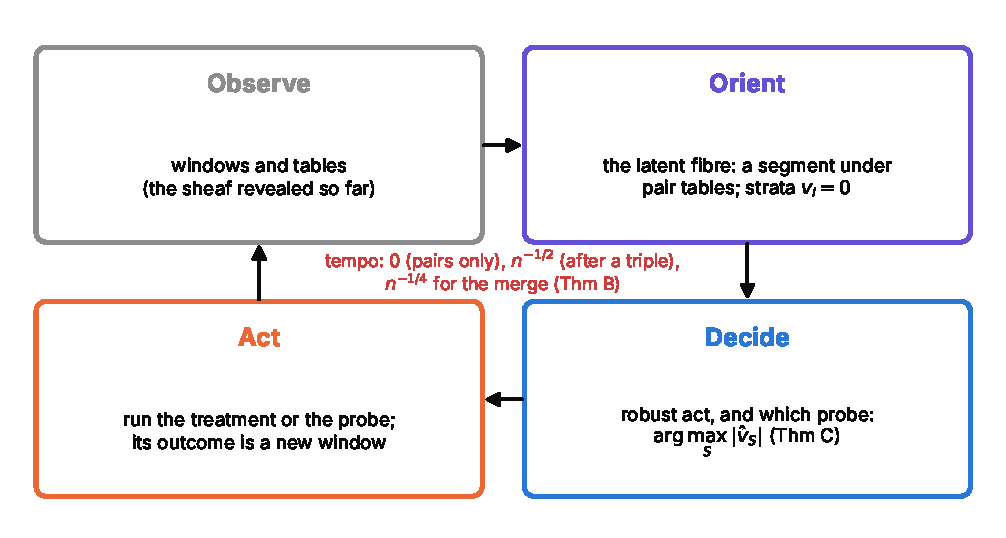
\includegraphics[width=0.8\linewidth]{fig_ooda.pdf}
\caption{The lab as an OODA loop on the geometry. The probe rule and the tempos are \cref{thm:C,thm:B}.}\label{fig:ooda}
\end{figure}

\section{Setup}\label{sec:setup}
Two latent types with weights $w_1=w$ and $w_2=1-w$ act on $m$ binary variables, such as harms. Type $j$ has harm probabilities
$a_j\in[0,1]^m$. The observed law is the mixture of the two product laws. Write
\[
\mu=w_1a_1+w_2a_2,\qquad d=a_1-a_2,\qquad v=\sqrt{w_1w_2}\,d,\qquad r=\frac{w_2-w_1}{\sqrt{w_1w_2}}=t-\frac1t,\quad t=\sqrt{w_2/w_1}.
\]
A \emph{window} $S$ is a set of variables whose joint table is observed. The central moments of the law are
$m_S=\mathbb E\prod_{i\in S}(x_i-\mu_i)$, and the law of the variables in a set $K$ is affine in $(\mu,(m_S)_{S\subseteq K})$.

\begin{lemma}[moment factorisation \cite{PG}]\label{lem:mom}
$m_S=v_S\,s_{|S|}(r)$, where $v_S=\prod_{i\in S}v_i$, $s_2=1$, $s_3=r$ and $s_{k+1}=r\,s_k+s_{k-1}$. In particular $s_k$ is a polynomial of
degree $k-2$.
\end{lemma}

The \emph{decision problem} follows Section 17 of \cite{PG}. An act $a$ has utility $u_a$ on outcomes, with values in
$[u_{\min},u_{\max}]$. Two kinds of cover are used: the \emph{pair cover} (all single and pair tables) and covers with triples added. The
\emph{latent fibre} $X_C$ of a cover $C$ is the set of two-type explanations consistent with its tables. The worked act throughout is
``treat'', with $u=1-1.2\,[E]$ where $E$ is any harm among three variables, against ``nothing'' with $u=0$.

\section{Theorem A: the hiding segment}\label{sec:A}
\begin{theorem}[hiding segment]\label{thm:A}
Let $m\ge3$, and suppose at least three coordinates of $v$ are non-zero.
\begin{enumerate}
\item[(a)] The pair cover determines $\mu$, and $v$ up to a common sign. Its latent fibre is, up to relabelling the types, the segment
\[X_{\rm pair}=\{(w(t),\,\mu+v\,t,\,\mu-v/t):\ t\in[t_-,t_+]\},\]
where $t_\pm$ are cut out by the box walls. For $v_i>0$ the constraints are $v_i/\mu_i\le t\le(1-\mu_i)/v_i$. For $v_i<0$ they are
$-v_i/(1-\mu_i)\le t\le\mu_i/(-v_i)$.
\item[(b)] Along the segment, the probability of any event on a set $K$ of $k$ variables is a polynomial in $r$ of degree at most $k-2$.
Its coefficient of $r^j$ involves only the products $v_S$ with $S\subseteq K$ and $|S|\ge j+2$.
\item[(c)] Hence robust (worst-case) values over the segment are attained at the box walls $t=t_\pm$, or at no more than $k-3$ interior
critical points. For $k=3$ only the walls count.
\end{enumerate}
\end{theorem}

\begin{proof}
(a) The pair moments are $m_{ij}=v_iv_j$. With three non-zero coordinates, $v_i^2=m_{ij}m_{ik}/m_{jk}$ fixes $|v_i|$, and the signs of
the products fix $v$ up to a global sign, which relabels the types. Given $(\mu,v)$, each $t>0$ gives $w=1/(1+t^2)$, $a_1=\mu+v\,t$ and
$a_2=\mu-v/t$, and all of them reproduce every single and pair table, since those depend only on $\mu$ and $v$. The box constraints are
linear in $t$ and $1/t$, so they cut out an interval.

(b) The law on $K$ is affine in the $m_S$ with $S\subseteq K$, and $m_S=v_S\,s_{|S|}(r)$ with $\deg s_{|S|}=|S|-2$
(\cref{lem:mom}).

(c) A polynomial of degree $k-2$ on an interval has its extremes at the ends or at roots of its derivative.
\end{proof}

The degree bound can drop on a stratum. If $v_i=0$, every product containing $i$ vanishes, so the terms they carry disappear. Study
11's registered prediction Q2 missed this (\cref{sec:lab}). \Cref{fig:segment}(c) shows what the segment means in practice: identical
pair tables come from a rare subgroup that differs a lot or from a common one that differs a little. For a regulator these are
different drugs.

\begin{figure}[!htbp]\centering
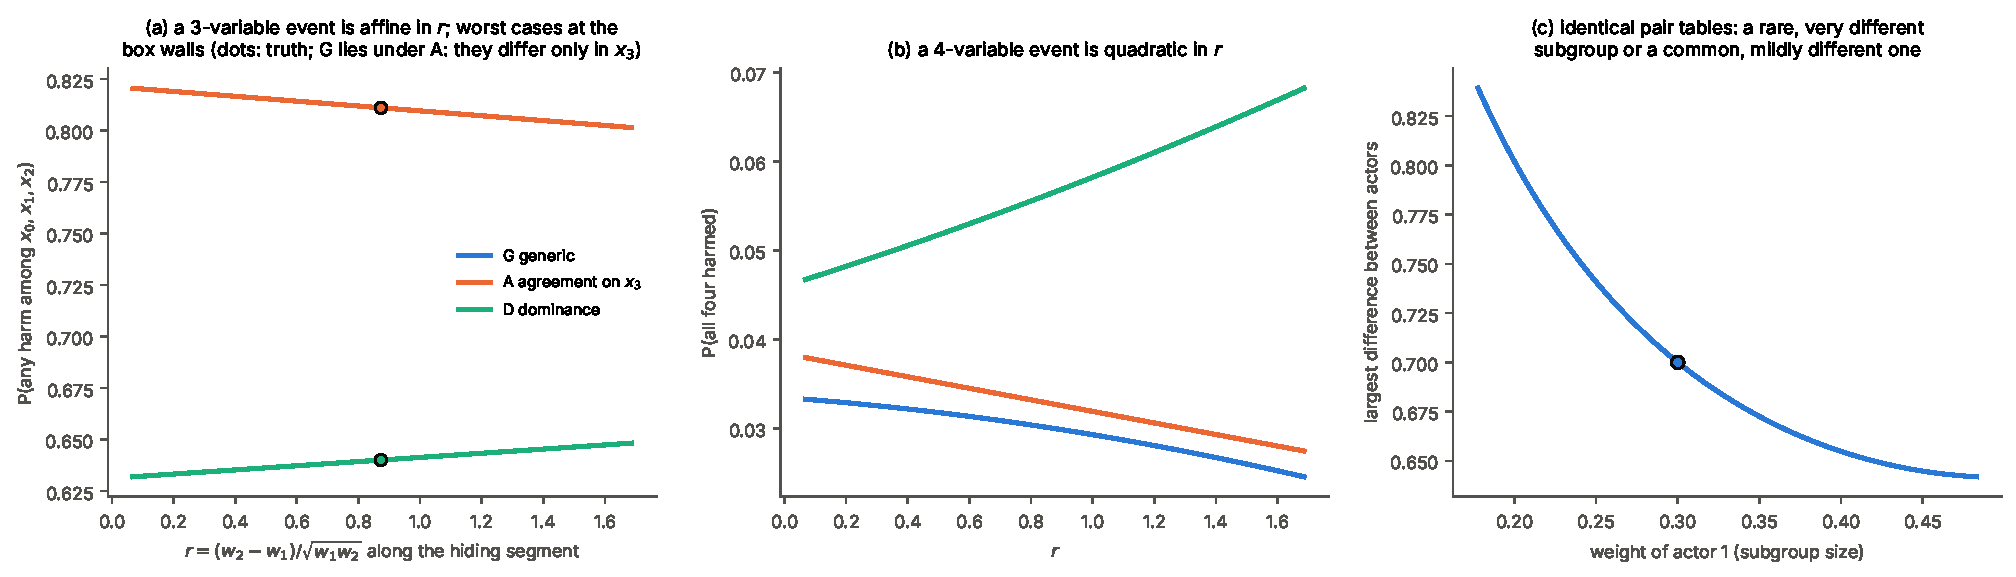
\includegraphics[width=\linewidth]{fig_segment.pdf}
\caption{Theorem A on the registered conditions. (a) A three-variable event is affine along the segment, so its worst case sits at a box
wall; dots mark the truth. (b) A four-variable event is quadratic. In condition A ($v_3=0$) it is affine (the stratum effect). (c) Along
the segment for condition G: the subgroup's size against how different it is.}\label{fig:segment}
\end{figure}

\section{Theorem B: three tempos}\label{sec:B}
\begin{theorem}[tempo]\label{thm:B}
Let each window be observed with $n$ independent samples.
\begin{enumerate}
\item[(a)] \emph{Pair-only disclosure: tempo zero.} The pair tables are the same at every point of the segment, so no estimator based
on them identifies $r$. The minimax error for $r$ stays at least half the segment's width for every $n$. The same holds for any
prediction whose $r$-coefficient is non-zero.
\item[(b)] \emph{After one triple window $S$ with $v_S\ne0$.} $r=m_S/v_S$, and every parameter is a smooth function of window
moments with non-vanishing Jacobian. So all are estimated at rate $n^{-1/2}$, and the constant for $r$ is proportional to
$\sigma_S/|v_S|$ with $\sigma_S^2=\mathbb E[\prod_{i\in S}(x_i-\mu_i)^2]$.
\item[(c)] \emph{Relations.} Agreement on one variable ($v_i=0$ while at least two other coordinates are non-zero) is regular:
$v_i=m_{ij}/v_j$ is estimated at $n^{-1/2}$. At the merge ($v=0$, identical types) the separation $\|v\|$ is estimated only at rate
$n^{-1/4}$, which is optimal \cite{Chen1995}. Predictions of observed events stay at $n^{-1/2}$ everywhere.
\end{enumerate}
\end{theorem}

\begin{proof}
(a) is \cref{thm:A}(a). Two truths at the ends of the segment produce the same distribution of the data, so Le Cam's two-point bound
gives minimax risk at least half their distance.

(b) is the delta method.

(c) At $v=0$ the pair moments are pure noise of size $n^{-1/2}$. A rank-one fit returns $\hat v\hat v^\top$ of that size, so
$\|\hat v\|\asymp n^{-1/4}$; Chen \cite{Chen1995} shows this rate is optimal for mixtures at coincidence. For agreement, $\hat v_i$ is a
ratio of moments whose denominator is bounded away from zero.
\end{proof}

In the design discussion we had predicted the slow rate for agreement on one variable. The proof shows it belongs to the merge only.
The registration of Study 11 records the correction, which was made before any run (\cref{sec:lab}). Another stratum is not
identifiable at all: if the types differ on at most two variables, the law depends on $v$ only through one product. The same is true
of an absent type ($w_2=0$), whose law is exactly that of the merge. So these relations are invisible in any data, not merely slow to
estimate (R4 in \cref{tab:study}).

\begin{figure}[!htbp]\centering
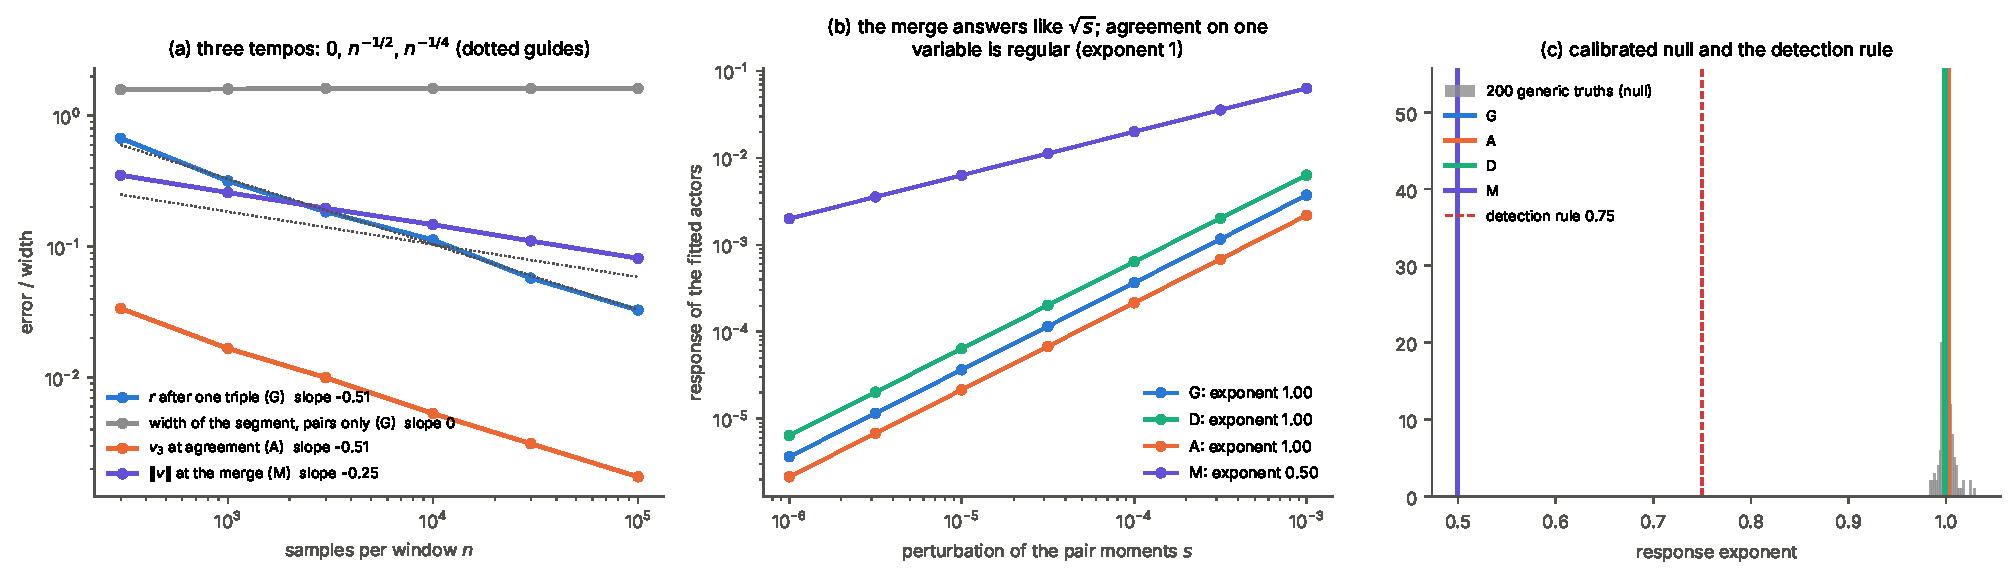
\includegraphics[width=\linewidth]{fig_tempo.pdf}
\caption{Theorem B. (a) Learning curves: the weight is never learned from pairs (flat). After one triple it converges at $n^{-1/2}$.
Agreement on one variable is also $n^{-1/2}$, and the merge is $n^{-1/4}$. (b) The same signatures as response exponents to deterministic
perturbations of the pair tables. (c) The null distribution of exponents over 200 generic truths, and the registered detection rule.}\label{fig:tempo}
\end{figure}

\section{Theorem C: the value of a probe}\label{sec:C}
For a cover $C$ with fibre $X_C$, take a probe $w'$ whose exact outcome reveals the post-probe fibre $X_{C\cup w'}(x)\ni x$. Its
\emph{minimax value} is
\[
\mathrm{VOI}(w')=\min_{x\in X_C}\ \max_a\ \min_{x'\in X_{C\cup w'}(x)}U(a,x')\;-\;\max_a\min_{x\in X_C}U(a,x),\qquad U(a,x)=\mathbb E_xu_a .
\]
This is Wald's minimax applied to information: the gain in the worst case when the adversary picks the truth. It is the minimax
analogue of Howard's value of information \cite{Howard1966}, and by the minimax inequality it is non-negative. Replacing $U$ by minus
Savage's regret, $-\bigl(\max_bU(b,x)-U(a,x)\bigr)$, gives the \emph{regret value} $\mathrm{VOI}_{\mathrm{reg}}$ \cite{Savage1951}.

\begin{theorem}[stratified VOI and the mandated window]\label{thm:C}
Let $C$ be the pair cover and $Z=\{i:v_i=0\}$ the coincident set. Let $w'$ be a triple window on $S$.
\begin{enumerate}
\item[(1)] On the independence stratum ($v=0$), $\mathrm{VOI}(w')=0$ for every probe.
\item[(2)] If $S$ meets $Z$, then $v_S=0$, the probe does not pin $r$, and $\mathrm{VOI}(w')=0$.
\item[(3)] If $S$ avoids $Z$, the probe pins the point, and $\mathrm{VOI}(w')=g$, the minimax gap of perfect information on the segment:
$g=\min_x\max_aU-\max_a\min_xU\ge0$, the same for every such $S$. It is zero exactly when $U$ has a saddle point on acts $\times$
segment, in particular whenever all acts have their worst case at a common point. For an event on three variables every $U(a,\cdot)$
is affine in $r$ (\cref{thm:A}), so its worst case is at a wall, and $g>0$ needs two acts with worst cases at opposite walls. The regret
value is $\mathrm{VOI}_{\mathrm{reg}}(w')=\min_a\max_x\bigl(\max_bU(b,x)-U(a,x)\bigr)$, which is positive exactly when no act is
optimal along the whole segment.
\item[(4)] With $n$ samples, the post-probe set is $\{x:|r(x)-\hat r|\le c\,\sigma_S/(|v_S|\sqrt n)\}$. So the value is non-decreasing in
the signal $|v_S|\sqrt n/\sigma_S$, and it vanishes as the truth approaches any plane $\{v_i=0:i\in S\}$.
\item[(5)] The pair tables estimate $v$, so the regulator can name the best probe, $\arg\max_S|\hat v_S|/\hat\sigma_S$, before
running it.
\end{enumerate}
\end{theorem}

\begin{proof}
(1) The law is a product, and every point of the fibre gives the same predictions.

(2) and (3) follow from \cref{thm:A} and $m_S=v_S\,r$. A pinned point gives $\max_aU(a,x)$ for each $x$, and the adversary minimises
over $x$. Hence $g=0$ iff $\min_x\max_aU=\max_a\min_xU$, which is the saddle condition; a common worst point $x_0$ gives
$\min_x\max_aU\le\max_aU(a,x_0)=\max_a\min_xU$. After pinning, the regret is $0$, so the regret value is the pre-probe minimax
regret.

(4) The value is monotone in the post-probe set: a smaller set has a larger worst case. That set shrinks as $|v_S|\sqrt n/\sigma_S$
grows, by \cref{thm:B}(b).

(5) is immediate from (4).
\end{proof}

\begin{corollary}[unravelling]\label{cor:unravel}
Suppose a sponsor can reveal a triple table verifiably and at no cost, the regulator approves only if the worst case over the revealed
fibre meets the requirement, and the sponsor wants approval. Then every sponsor whose true outcome meets the requirement reveals the
triple. Approval then coincides with full information.
\end{corollary}

\begin{proof}
For a safe sponsor, revealing gives approval, because the exact value meets the requirement. Not revealing gives approval only if the
worst case over the segment does, and that is never better. For a harmful sponsor neither choice gives approval. This is Milgrom's
unravelling argument \cite{Milgrom1981,Grossman1981} on the segment.
\end{proof}

The rule borrowed is classical; the structure that makes it apply is the segment. The same structure explains when skepticism fails.
If the reported tables come from a different population, for example pooled with a benign one, the skeptic's worst case is taken over
the wrong segment (D4).

\begin{proposition}[when evidence can hurt]\label{prop:monotone}
At level one, with the contamination model of \cite{PG}, let $C\subseteq C'$. For every act, the robustness on $C'$ is at least the
robustness on $C$, unless the act is vacuous on $C'$ (robustness $-\infty$). So a new window can lower a robust decision maker's
robustness only by making the evidence vacuous for that act.
\end{proposition}

\begin{proof}
$E_\alpha(C')\subseteq E_\alpha(C)$, so the robust value $V_{C'}(a;\alpha)\ge V_C(a;\alpha)$ for every $\alpha\le\lambda^*(C')$, and
$V$ is monotone in $\alpha$. If $V_{C'}(a;\lambda^*(C'))\ge u_0$, the set of admissible contaminations on $C'$ contains that on $C$
intersected with $[1-\lambda^*(C'),1]$, and it starts no lower. Otherwise the act is vacuous on $C'$.
\end{proof}

This corrects an earlier statement of ours that new evidence can lower robustness gradually. Under ambiguity aversion, the value of
information can be negative \cite{AlNajjarWeinstein2009,Siniscalchi2011}. Here that happens only by a jump to vacuity, as when a
strongly conflicting trial drives $\lambda^*$ below the threshold of \cite[Prop.~33]{PG}. Study 11's registered prediction L8 expected
a gradual loss and failed. A post-hoc check confirms the proposition (\cref{sec:lab}).

\begin{figure}[!htbp]\centering
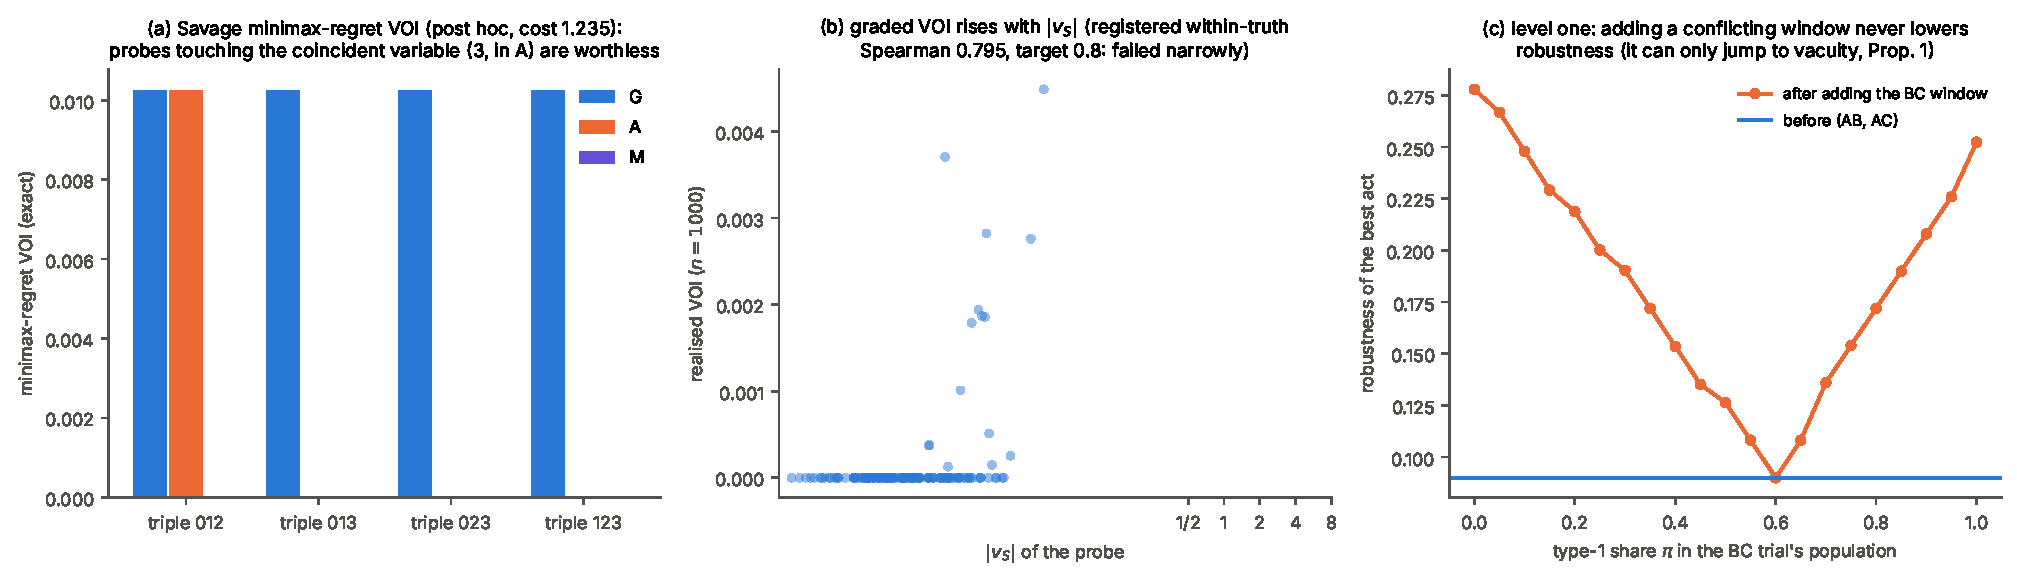
\includegraphics[width=\linewidth]{fig_voi.pdf}
\caption{Theorem C. (a) Exact regret VOI per triple (post hoc, harm cost $1.235$, at which the best act changes along G's segment).
In A, the triples containing the coincident variable are worthless; in M every probe is. The Wald gap $g$ is $0$ here at every cost,
because both acts have their worst case at the same wall: a saddle point. (b) Graded VOI at $n=1000$ against $|v_S|$, for random truths where some probe matters. (c) Level one: robustness after adding
a conflicting window, over a family of populations. It never falls except by vacuity (\cref{prop:monotone}).}\label{fig:voi}
\end{figure}

\section{Theorem D: the decision on the segment}\label{sec:D}
Theorems A--C say what is hidden, how fast it is revealed and what a probe is worth. They do not say how to choose an act on the
segment, whether that choice is stable, or when the evidence settles it. This section does, for two types on the pair cover.

Write $R=[r_-,r_+]$ for the segment in the coordinate $r$, and $U_a(r)$ for the expected utility of act $a$ at the explanation with
parameter $r$. Let $u_a$ depend on the variables in a set $T$ with $|T|=k$, and let $\chi(x)=\prod_{i\in T}(2x_i-1)$. For an evidence
interval $I\subseteq R$ let $W_a(I)=\min_IU_a$, the act's worst value on $I$. The \emph{set rule} $\sigma(I)$ chooses, among the acts
with $W_a(I)\ge u_0$, one with the largest worst value, and abstains if there is none. The \emph{info-gap rule} \cite{BenHaim2006} needs a
nominal point $\hat r$ and chooses the act with the largest horizon
$\alpha_a(\hat r)=\sup\{h:W_a([\hat r-h,\hat r+h]\cap R)\ge u_0\}$. The \emph{oracle act} is $a^\circ=\sigma(\{r_0\})$ at the true point
$r_0$.

\begin{theorem}[the decision on the segment]\label{thm:D}
\begin{enumerate}
\item[(1)] \emph{Existence.} $U_a$ is a polynomial in $r$ of degree at most $k-2$, and $W_a(R)$ is attained at a wall or at one of at
most $k-3$ interior critical points. For $k=3$,
\[U_a(r)=U_a(\hat r)+\beta_a(r-\hat r),\qquad \beta_a=v_T\sum_xu_a(x)\chi(x),\]
the top Walsh coefficient of the utility times $v_T$. So an act meets the requirement on the whole segment iff it does at both walls, and
one exists iff $\max_a\min\{U_a(r_-),U_a(r_+)\}\ge u_0$.
\item[(2)] \emph{Uniqueness, and flat acts.} $\sigma(R)$ is unique unless two admissible acts have equal worst values. For $k=3$ the
horizon is $\alpha_a=(U_a(\hat r)-u_0)/|\beta_a|$, or $+\infty$ when the act is admissible on the whole segment. So info-gap prefers acts
with a small top Walsh coefficient, the acts least exposed to the hidden triple moment. When two or more acts are admissible on all of
$R$ their horizons tie at $+\infty$, and only the nominal value separates them. The info-gap choice and the set-rule choice can differ.
\item[(3)] \emph{Invariance and stability.} $\sigma(R)$ is a function of the pair tables alone, so it is the same for every law on the
fibre: a perturbation the decision maker cannot detect never changes it. An info-gap choice before the probe is not invariant in this
sense, because pair tables carry no information about $r$, so its nominal point is a convention; the midpoint in $r$ and the midpoint in
$t$ can give different acts. Under detectable perturbations $\sigma(R)$ changes only where some $W_a(R)$ crosses $u_0$ or two worst
values cross; these are algebraic hypersurfaces in the pair moments, and the distance to them is the decision's stability margin.
\item[(4)] \emph{Settling} ($k=3$). After a triple window with $n$ draws per window, the post-probe set is
$I_n=[\hat r-h_n,\hat r+h_n]\cap\hat R$ with $h_n=z\hat\tau/\sqrt n$, where $\hat\tau$ estimates the asymptotic standard deviation
$\tau$ of $\sqrt n\,\hat r$ (\cref{thm:B}). For an interval $[c-h,c+h]$ inside $R$, $\sigma$ chooses $a^\circ$ iff every constraint
\[g_j(c)-\gamma_jh\ge0\]
holds, where $g_0=U_{a^\circ}-u_0$ and $\gamma_0=|\beta_{a^\circ}|$, and $g_b=U_{a^\circ}-U_b$ and $\gamma_b=|\beta_{a^\circ}|-|\beta_b|$
for every other act $b$. Hence:
\begin{enumerate}
\item[(a)] The \emph{settling radius} is $d=\min_{\gamma_j>0}g_j(r_0)/\gamma_j$. Constraints with $\gamma_j\le0$, against steeper acts,
never bind as $h$ grows.
\item[(b)] $P(\sigma(I_n)=a^\circ)\to P\bigl(g_j(r_0)\sqrt n+\xi_j\ge\gamma_jz\tau\ \text{for all }j\bigr)$, with $\xi\sim N(0,\Sigma)$ the
delta-method limit of the plug-in constraints. If one constraint binds, the median settling size is
\[n^*=(z\tau/d)^2,\]
whatever $\Sigma$ is.
\item[(c)] On the stratum $g_j(r_0)=0$, where the truth sits on a crossing or on the requirement, the settling probability tends to
the plateau $\Phi(-\gamma_jz\tau/s_j)<1$, with $s_j^2=\Sigma_{jj}$. The decision never settles.
\end{enumerate}
\end{enumerate}
\end{theorem}

\begin{proof}
(1) For binary variables the law of $T$ has the exact expansion
$P_T(x)=\sum_{S\subseteq T}m_S\prod_{i\in S}(2x_i-1)\prod_{i\in T\setminus S}p_i(x_i)$, with $m_\emptyset=1$, $m_{\{i\}}=0$ and
$p_i(1)=\mu_i$. By \cref{lem:mom}, $m_S=v_Ss_{|S|}(r)$ has degree $|S|-2$, so $U_a$ has degree at most $k-2$. Its minimum on an interval
is at an endpoint or at a root of $U_a'$, of which there are at most $k-3$. For $k=3$ only $S=T$ depends on $r$, through $m_T=v_Tr$, and
its coefficient is $\sum_xu_a(x)\chi(x)$.

(2) For affine $U_a$, $W_a([\hat r-h,\hat r+h])=U_a(\hat r)-|\beta_a|h$ until the interval meets the wall on the downhill side; from then
on the worst value is the wall value, which is at least $u_0$ if it is reached first. Solving for $h$ gives the horizon.

(3) $R$, $\mu$ and $v$ are determined by the pair tables (\cref{thm:A}), and so are the $U_a$. $\sigma$ depends on the $W_a(R)$ only
through the order of the admissible ones, which changes only at the stated equalities. The non-invariance of a nominal choice is an
example (check DS6).

(4) For affine $U_a$, $W_a([c-h,c+h])=U_a(c)-|\beta_a|h$. The set rule chooses $a^\circ$ iff $W_{a^\circ}\ge u_0$ and
$W_{a^\circ}\ge W_b$ for all $b$, since an act with $W_b>W_{a^\circ}\ge u_0$ is admissible; these are the constraints. At $c=r_0$ they
hold exactly for $h\le d$, which is (a). The plug-in constraints $\hat g_j$ are smooth functions of the window tables, so
$\sqrt n(\hat g_j-g_j)\to N(0,\Sigma)$ by the delta method, and $\hat\tau\to\tau$. With one binding constraint the settling probability
tends to $\Phi\bigl((g_j\sqrt n-\gamma_jz\tau)/s_j\bigr)$, which equals $1/2$ exactly when $\sqrt n=\gamma_jz\tau/g_j=z\tau/d$; this is
(b). If $g_j=0$ the argument is $-\gamma_jz\tau/s_j$ for every $n$, which is (c).
\end{proof}

Three remarks fix the scope.
\begin{itemize}
\item \emph{Settling is not expiry.} In the main note's time-varying decisions, a decision expired when a new distinction entered the
  utility, and no radius predicted it \cite[Section~17]{PG}. Settling is driven by evidence alone, and it is computable.
\item \emph{Level one and level two together.} If conflicting windows are added, the contamination model of \cite{PG} applies on top
  of the segment, and its vacuity bound \cite[Prop.~36]{PG} can make every act inadmissible. A theorem for the combined worst case is
  open.
\item \emph{What is not covered.} Parts (2) and (4) are for utilities on three variables, where $U_a$ is affine. For four variables
  $U_a$ is quadratic, and settling has to track the interior critical point. More than two types, and other covers, are open.
\end{itemize}
Checks DS1--DS9 verify the parts exactly or by bisection on random truths (\cref{sec:lab}).

\section{Studies 11 and 11b}\label{sec:lab}
\subsection*{Study 11: Theorems A--C and the disclosure game}
The study was pre-registered and frozen with SHA-256 before any registered condition was computed
(\texttt{engine/study11\_lab/PREREG\_study11.md}). Three amendments were made before the run, and each is logged in the registration:
\begin{itemize}
\item the correction to Theorem B noted above;
\item two design fixes to illustrations;
\item one change to L6, prompted by a smoke test on an invented truth, which showed that the minimax VOI can be zero everywhere; L6
  was reduced to the zero pattern and a common value.
\end{itemize}
One deviation arose during the run. For some truths the pooled tables of the disclosure game have no two-type explanation at all, and
the rule adopted (reject) is logged in \texttt{DEVIATIONS\_study11.md}. \Cref{tab:study} lists the predictions.

\begin{table}[!htbp]\centering\small
\begin{tabular}{p{0.06\linewidth}p{0.6\linewidth}p{0.26\linewidth}}\toprule
& prediction & outcome\\\midrule
Q1 & pair rank $2m$, plus one triple $2m+1$ ($m=3,4,5$) & holds\\
Q2 & a 3-variable event is affine; the 4-variable event is quadratic, not affine (G, A, D) & \textbf{fails for A}: affine there, since $v_{0123}=0$\\
Q3 & extremes of the 3-variable event at the walls & holds\\
R1--R3 & response exponents: G $1.00$, D $1.00$, A $1.00$ (agreement is regular), M $0.50$ & hold\\
R4 & absent type = merge: identical tables & holds\\
R5 & null band and detection rule & holds\\
R6 & agreement rests exactly on the windows containing the variable & holds\\
L1--L4 & slopes: $r$ after a triple $-0.51$; $v_3$ at agreement $-0.51$; merge $-0.25$; pair-only width flat & hold\\
L5 & the probe rule matches the oracle; it avoids the coincident variable & holds\\
L6 & exact VOI: zero pattern and common value & holds ($g=0$: a saddle point)\\
L7 & graded VOI monotone in $|v_S|$ within a truth (mean Spearman $\ge0.8$) & \textbf{fails narrowly} ($0.795$)\\
L8 & some conflicting window lowers robustness (drug family) & \textbf{fails}; explained by \cref{prop:monotone}\\
D1--D7 & disclosure game (\cref{sec:game}) & all hold\\\midrule
I1, I3 & illustrations: bandit reaches the rule; catch-up is finite & hold\\
I2 & illustration: gradient play does not approach the mixed equilibrium & \textbf{fails}: it approaches, then cycles\\\bottomrule
\end{tabular}
\caption{Study 11: registered predictions and outcomes.}\label{tab:study}
\end{table}

The three failures say more than the passes.
\begin{itemize}
\item \emph{Q2} failed because the registration ignored the stratum effect that \cref{thm:A}(b) states.
\item \emph{L7} failed narrowly because the registered statistic ranked probes by $|v_S|$ alone, while the theorem's signal is
  $|v_S|/\sigma_S$. Post hoc, on fresh truths, the within-truth correlation is $0.85$ with $|v_S|$ and $0.87$ with
  $|v_S|/\sigma_S$.
\item \emph{L8} failed because the registered expectation was false: robustness cannot fall gradually (\cref{prop:monotone}). Post hoc,
  every member of the family satisfies monotonicity, computed by exact bisection. A strongly conflicting window ($\lambda^*=0.30$) makes
  every act vacuous, which is the only way down.
\end{itemize}

\begin{figure}[!htbp]\centering
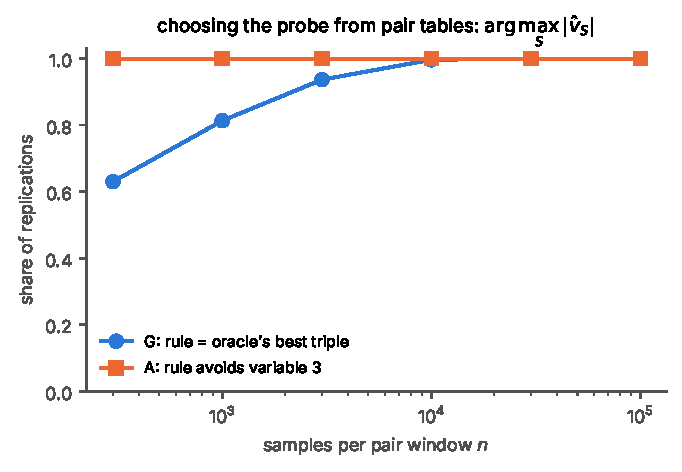
\includegraphics[width=0.48\linewidth]{fig_probe.pdf}
\caption{Choosing the probe from pair tables. The rule $\arg\max_S|\hat v_S|$ matches the oracle's choice in $99.7\%$ of replications at
$n=10^4$. In condition A it never picks a triple containing the coincident variable.}\label{fig:probe}
\end{figure}

\subsection*{Study 11b: when the decision settles}
Study 11b tests \cref{thm:D}(4). It was registered and frozen with SHA-256 before any registered design was simulated
(\texttt{engine/study11b\_settle/PREREG\_study11b.md}), after the engine checks and two smoke runs on an invented design. The first smoke
run showed that a second constraint close to the binding one moves the median above $n^*$, as \cref{thm:D}(4b) allows; the designs were
then fixed so that one constraint binds.

There are five designs on two truths. In each, a treatment act ($u=b-[\text{any harm}]$, or $b-[\text{at least two harmed}]$) faces a
flat conservative act ($u=b-[\text{variable 0 harmed}]$, $\beta=0$), or the requirement alone. Before the probe the set rule chooses the
conservative act, or abstains; the oracle chooses the treatment. D3 puts the boundary on the other side of $r_0$, D5 uses a second
truth, and D4 puts the truth on the crossing, the stratum $d=0$. Each cell has 4000 replicates; each replicate samples three pair
windows and the triple window independently. The regulator uses the plug-in $\hat\tau$ and $z=1.96$.

\begin{table}[!htbp]\centering\small
\begin{tabular}{p{0.06\linewidth}p{0.6\linewidth}p{0.26\linewidth}}\toprule
& prediction & outcome\\\midrule
S1 & settling rate within $0.05$ of the delta-method prediction in $\ge18$ of 20 cells, and within $0.08$ in all & holds: 20 of 20, largest gap $0.014$\\
S2 & empirical median settling size within a factor $1.25$ of $n^*=(z\tau/d)^2$ & holds: ratios $0.94$, $1.08$, $1.00$, $0.93$\\
S3 & D4 stays on the predicted plateau (within $0.05$) and does not rise between $n=3000$ and $10^5$ & holds: largest gap $0.021$; $0.27$ at both ends\\
S4 & without the triple, the set rule on the estimated segment picks the population's pre-probe act ($\ge95\%$) & holds: $98$--$100\%$\\\bottomrule
\end{tabular}
\caption{Study 11b: registered predictions and outcomes.}\label{tab:study11b}
\end{table}

All four predictions held (\cref{tab:study11b,fig:decide}). The predicted medians were $n^*=3270$ (D1, D2), $6410$ (D3) and $2001$ (D5).
The settling curves are shallow: at $8n^*$ between $85\%$ and $99\%$ of replicates had settled. The reason is in \cref{thm:D}(4b): the
plug-in constraints carry noise from the pair tables as well as from $\hat r$, and that noise widens the curve without moving its
median. On the stratum (D4) the share settled stayed near $0.28$ from $n=10^3$ to $10^5$, as predicted. At most $0.75\%$ of replicates
had pair tables with no two-type explanation.

\begin{figure}[!htbp]\centering
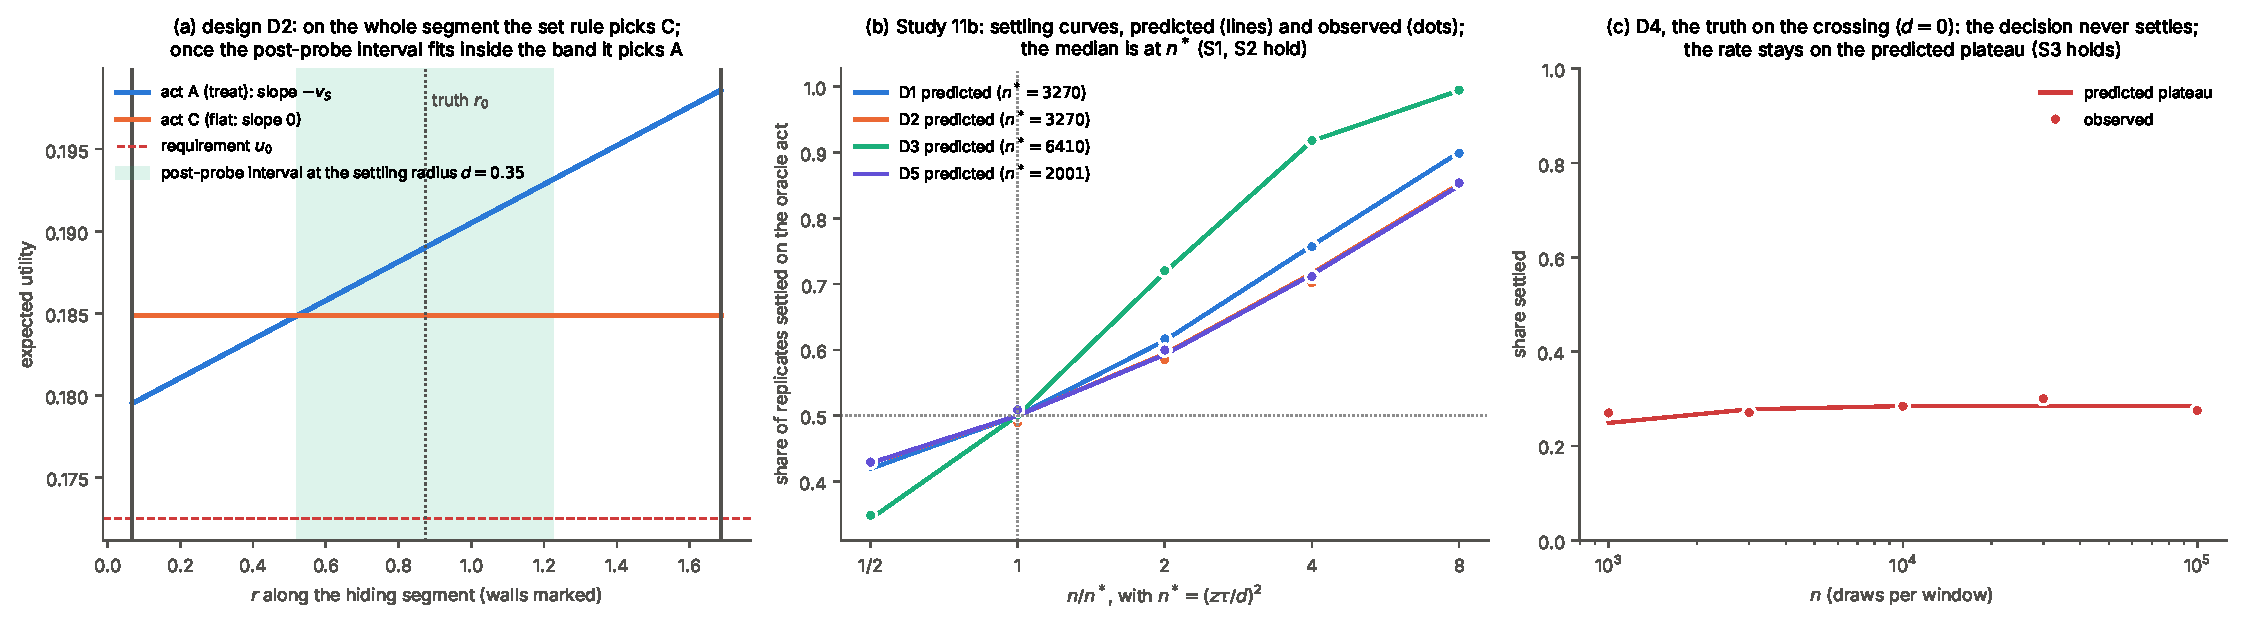
\includegraphics[width=\linewidth]{fig_decide.pdf}
\caption{Theorem D and Study 11b. (a) Design D2: the treatment's line and the flat act's line on the segment. On the whole segment the
set rule picks the flat act; once the post-probe interval fits within the settling radius it picks the treatment. (b) Settling curves
against $n/n^*$: predicted (lines) and observed (dots); each crosses one half at $n^*$. (c) The stratum $d=0$: the share settled stays on
the predicted plateau and never rises to one.}\label{fig:decide}
\end{figure}

\section{Theorem D and the ring of contingency tables}\label{sec:ehrhart}
The companion \cite{CouplingAlgebras} puts the geometry of couplings into a graded ring: the Ehrhart ring of a polytope of tables with
rational margins. Its degree-$k$ piece has the integer tables with $k$ times the margins as a basis. Its Hilbert function counts them,
and the count crosses the walls of the margin space by one binomial term at a time. A reviewer asked two questions about it. Is the
decision functional of \cref{thm:D}, the worst case of an act over the hiding set, a section of this ring? And is the settling size
$n^*$ a wall-crossing? The short answers are no and no. The ring does give two things, though: the correct algebraic form of the worst
case, and an exact probe that settles sooner. This section works it out for three binary variables, the case of \cref{thm:D}(4).

\paragraph{The fibre.} Fix the three pair tables of a law $P$ on $\{0,1\}^3$. The laws that share them form a segment
$P+\varepsilon\chi$, with $\chi(x)=\prod_i(2x_i-1)$. This is the no-three-way-interaction model. Its toric ideal is principal, generated by
the single quartic $p_{000}p_{011}p_{101}p_{110}-p_{001}p_{010}p_{100}p_{111}$ (Macaulay2, check EH1), so $\chi$ is its only Markov
move. Moving along the fibre moves the triple moment at unit speed, because
\[
m_T(P+\varepsilon\chi)-m_T(P)=\varepsilon\sum_x\chi(x)\prod_i(x_i-\mu_i)=\varepsilon\prod_i\bigl((1-\mu_i)+\mu_i\bigr)=\varepsilon .
\]
So the fibre is an interval of $m_T$, ended where a cell reaches zero. If $P$ has denominator $N$, then at sample size $n=kN$ the integer
tables with the pair tables of $nP$ are the points $nP+j\chi$, $j\in\mathbb Z$, a lattice of step $1/n$ in $m_T$. The hiding set $R$
of \cref{thm:A} is the part of this interval where a two-type explanation exists, $m_T\in v_T\,[r_-,r_+]$.

\begin{proposition}[the hiding set inside the ring]\label{prop:ehrhart}
For three binary variables and a two-type law $P$ with denominator $N$:
\begin{enumerate}
\item[(i)] The integer tables with the pair tables of $kNP$ are the lattice points of $k$ times a lattice segment of length $\ell$. Their
number is the Ehrhart polynomial $k\ell+1$, the degree-$k$ Hilbert function of the ring.
\item[(ii)] $R$ is a strict sub-segment. Its ends are where some $a_{ji}$ reaches $0$ or $1$, while every cell of the law is still
positive. Those ends are algebraic numbers and generally irrational. So the number of tables in $kR$ is not an Ehrhart polynomial, and
not even a quasi-polynomial.
\item[(iii)] The expected utility of an act on the three variables is affine on the fibre, $U_a=U_a(P)+c_a\,(m_T-m_T(P))$. Its slope is
the Walsh coefficient $c_a=\sum_xu_a(x)\chi(x)$, and $\beta_a=v_Tc_a$ in the coordinate $r$.
\end{enumerate}
\end{proposition}

\begin{proof}
(i) Every cell of a table with the given pair tables is an integer plus or minus one free integer, so the fibre is $T_0+\mathbb Z\chi$,
cut by $T_0+j\chi\ge0$. The ends are integers, and dilating by $k$ multiplies them by $k$. (ii) The ends of $R$ are the ends of
\cref{thm:A}'s box, where a coordinate of $a_1=\mu+vt$ or $a_2=\mu-v/t$ reaches $0$ or $1$; a cell of the mixture vanishes only if both
components vanish there. The count is $\lfloor n\,(R_+-m_0)\rfloor-\lceil n\,(R_--m_0)\rceil+1$. With irrational ends, its second
differences at any fixed period do not vanish. (iii) This is the computation above with $u_a$ in place of the moment.
\end{proof}

For the worked truth $w=\tfrac25$, $a_1=(\tfrac45,\tfrac3{10},\tfrac7{10})$, $a_2=(\tfrac15,\tfrac7{10},\tfrac3{20})$, the denominator is
$N=5000$. The fibre is $m_T\in[-0.0671,\,0.0609]$, a lattice segment of 640 steps. The hiding set $R=[-0.0214,\,0.0100]$ is $25\%$ of
it (\cref{fig:ehrhart}(a)).

\begin{proposition}[the decision functional and the ring]\label{prop:tropical}
\begin{enumerate}
\item[(i)] \emph{Not a section, but a tropical limit.} The worst value $W_a$ is a minimum of linear forms, so it is not an element of the
ring. It is the limit of a weighted count over the same basis of tables:
\[
\min_{T}U_a(T)-\frac{\log\#}{s}\ \le\ -\frac1s\log\sum_{T}e^{-sU_a(T)}\ \le\ \min_{T}U_a(T),
\]
where $T$ runs over the tables in $nR$ (or in the whole fibre) and $\#$ is their number. As $s\to\infty$ the middle term tends to the
lattice minimum. That minimum is $W_a$ exactly over the fibre, whose ends are lattice points, and within $|c_a|/n$ over $R$.
\item[(ii)] \emph{Over the whole fibre the worst case is an integer programme.} Take the quartic, oriented so that its leading term is
the costlier side. Its normal form (Conti--Traverso) is the table that minimises $U_a$. As a function of the pair tables this minimum is
piecewise linear. It breaks only where the binding cell changes, and those are the walls where the fibre's length, the leading
coefficient of the table count, breaks too. So a skeptic who allows every law with the given pair tables has decision walls that are
linear on each chamber of \cite{CouplingAlgebras}. The set rule on $R$ has algebraic walls instead, because positivity of the
explanation, not of the table, ends $R$.
\item[(iii)] \emph{$n^*$ is not a wall-crossing.} Raising $n$ moves the margins along a ray, and chambers are cones. So the table count
stays one polynomial, and no wall is crossed. The lattice is still visible at $n^*$, though. The truth sits
$n^*d\,|v_T|=(z\tau)^2|v_T|/d$ lattice steps from the decision wall: about ten in Study 11b's designs. The conditional law of the
position has standard deviation $\tau_c|v_T|\sqrt{n^*}$, about five steps.
\item[(iv)] \emph{The exact probe is the efficient one.} Given its own pair tables, the triple window is a lattice point on its fibre.
Its conditional law is the exponential family $\propto e^{\psi j}/\prod_x(T+j\chi)_x!$ in the three-way log odds ratio
$\psi=\sum_x\chi(x)\log p_x$. This is the sample space of Fisher's exact test in \cite[Thm.~7.1(iv)]{CouplingAlgebras}, tilted. Mapping
$\psi$ to $r$ through the known pair tables gives an estimate with asymptotic standard deviation
\[
\tau_c=\frac{1}{|v_T|\sqrt{\sum_x1/p_x}}\ \le\ \tau_m ,
\]
where $\tau_m$ is that of the plug-in moment (with $v$ known). The inequality is Cram\'er--Rao along the fibre, because $\sum_x1/p_x$ is
the Fisher information of the move. So with the pair tables known, the exact probe settles at the smaller size $n^*_c=(z\tau_c/d)^2$.
\end{enumerate}
\end{proposition}

\begin{proof}
(i) Bound the sum between its largest term and $\#$ times its largest term. Over the fibre the minimum of an affine function is at an
end, and the ends are lattice points (\cref{prop:ehrhart}(i)). Over $R$ the nearest lattice point to an end is within $1/n$ of it.
(ii) The Gr\"obner basis of a principal ideal is its generator, and reduction by it applies the move against the cost while the table
stays nonnegative. The end it reaches is $\min_x$ of a linear form in the margins, taken over the cells with the right sign of $\chi$;
both this minimum and the fibre's length change formula exactly where the argmin changes. (iii) A ray $kNP$ has fixed binding cells
(check EH5). At $n^*$ the post-probe half-width $z\tau/\sqrt{n^*}$ equals $d$; in lattice steps that is $n^*d|v_T|$. (iv) The
conditional law is classical, with sufficient statistic $j$. The Fisher information of $P+\varepsilon\chi$ in $\varepsilon$ is
$\sum_x\chi(x)^2/p_x$. The plug-in moment is a regular estimator of $\varepsilon$ on this one-parameter model, so its variance is at least
the inverse information.
\end{proof}

Checks EH1--EH7 (\texttt{engine/check\_ehrhart.py}) verify each statement, as follows.
\begin{itemize}
\item EH1: the brute-force counts.
\item EH2: the quasi-polynomial test, for periods up to $12$.
\item EH3: the tropical bounds, on three acts.
\item EH4: Conti--Traverso against enumeration and linear programming, and the kinks along lines of margins.
\item EH5: the lattice reading of $n^*$.
\item EH6: $\tau_c\le\tau_m$ on 300 random truths, and a simulation of the conditional MLE.
\item EH7: the exactness of the conditional interval, coverage at least $0.95$ at every $\psi$.
\end{itemize}

\subsection*{Study 11c: settling with the exact conditional probe}
Proposition~\ref{prop:tropical}(iv) makes a prediction that can fail. A regulator who knows the pair tables and uses the exact
conditional interval for $\psi$ should settle at $n^*_c$, earlier than the plug-in regulator of Study 11b. But exact intervals are
conservative, and at $n^*$ the conditional law spans only a few lattice steps. Study 11c was registered and frozen with SHA-256 before
any registered design was simulated (\texttt{engine/study11c\_exact/PREREG\_study11c.md}), after the checks above and one smoke run on an
invented design. It reuses Study 11b's designs D2, D3, D5 and the stratum D4, with the pair tables known. One triple window feeds both
probes, and there are 2000 replicates per cell.

\begin{table}[!htbp]\centering\small
\begin{tabular}{p{0.06\linewidth}p{0.56\linewidth}p{0.30\linewidth}}\toprule
& prediction & outcome\\\midrule
E1 & exact probe's median settling size within a factor $1.25$ of $n^*_c=(z\tau_c/d)^2$ & holds: ratios $1.08$, $1.06$, $1.09$\\
E2 & exact probe's median below the plug-in probe's in every design & \textbf{fails}: D2 $2735<2799$, D3 $5285<5612$, but D5 $1954>1860$\\
E3 & exact settling rate within $0.06$ of the normal theory with $\tau_c$ at every $n$ & holds: largest gap $0.046$\\
E4 & D4 (stratum): exact rates at $n=3000$ and $10^5$ within $0.05$, both below one half & holds: $0.021$ and $0.020$ (plateau $0.025$)\\\bottomrule
\end{tabular}
\caption{Study 11c: registered predictions and outcomes.}\label{tab:study11c}
\end{table}

Three of the four predictions held, and one failed (\cref{tab:study11c}, \cref{fig:ehrhart}(d)). The exact probe settles close to
$n^*_c$, but always a little later. Its medians are $6$--$9\%$ above $n^*_c$, and its rate sits below the normal-theory curve at every
$n$ up to $4n^*_c$. This is the price of an exact interval: its coverage is at least $95\%$, never exactly $95\%$ (check EH7), and at
$n^*$ only a few lattice steps carry the conditional law.

E2 failed in one design. The efficiency gain is $(\tau_m/\tau_c)^2$ in sample size. That is $12\%$ for truth G, which beats the
conservativeness, so in D2 and D3 the exact probe settled first. For truth H the gain is $8\%$, and conservativeness ate it: in D5 the
exact probe settled $5\%$ later than the plug-in. So the exact probe is the efficient one in the limit, but not uniformly better at
$n^*$. A mid-$p$ interval, which is less conservative, is the natural repair. It was not registered, and it is not tested here.

On the stratum D4 neither probe settles. With the pair tables known, the plateau is the one-sided $2.5\%$ of \cref{thm:D}(4c), not
Study 11b's $0.27$. That larger value came from the noise in the estimated pair tables.

\begin{figure}[!htbp]\centering
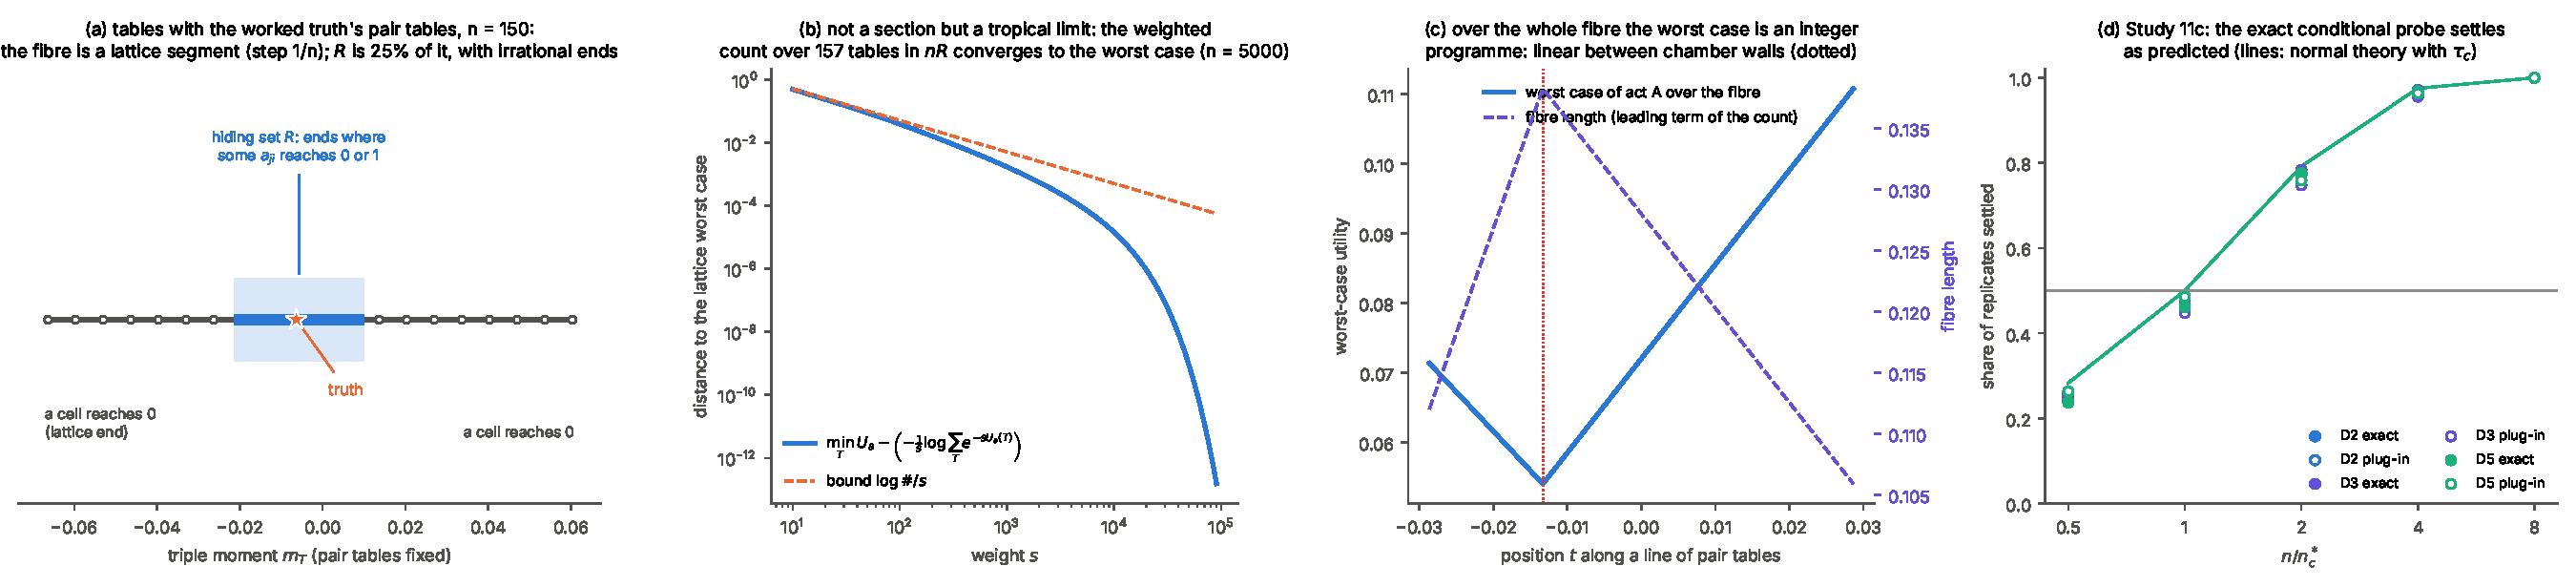
\includegraphics[width=\linewidth]{fig_ehrhart.pdf}
\caption{The decision and the ring of contingency tables. (a) The worked truth. The tables with its pair tables form a lattice segment
in $m_T$, shown at $n=150$ (dots). The hiding set $R$ (blue) is a quarter of it, ended by the explanation's positivity walls rather than
by a table's. (b) Act A's worst case over the tables in $nR$ as a tropical limit. The distance from the weighted count to the
lattice minimum stays below $\log\#/s$ and vanishes as $s$ grows. (c) Over the whole fibre, the worst case along a line of pair tables is linear between chamber walls
(dotted), where the fibre's length (dashed) also breaks. (d) Study 11c: settling with the exact conditional probe (filled) and the
plug-in probe (open) against $n/n^*_c$; the lines are the normal theory with $\tau_c$.}\label{fig:ehrhart}
\end{figure}

\paragraph{Gap 3, answered.}
\begin{itemize}
\item \emph{Is the decision functional a section?} No. The worst case is a tropical object: the $s\to\infty$ limit of a weighted Hilbert
  function. Over the whole margin fibre it is an integer programme solved by the toric ideal's Gr\"obner basis, and linear on chambers.
  Over the hiding set it is not polyhedral, because positivity of the explanation, not of the table, draws its walls.
\item \emph{Is $n^*$ a wall-crossing?} No. Raising $n$ moves along a ray inside one chamber. What does cross a wall is the truth leaving
  the stratum $d=0$, and that is a change of design, not of sample size.
\item \emph{What the ring contributes.} The ring supplies the exact sample space of the probe. Using it is the efficient way to settle,
  $\tau_c\le\tau_m$, and Study 11c measures what conservativeness costs at the few lattice steps that matter at $n^*$.
\end{itemize}


\section{For decision theory and the value of information}\label{sec:voi}
Knight's distinction \cite{Knight1921} between risk and uncertainty has a geometric form here. Under risk the fibre is a point; under
pair-only disclosure it is a segment, and nothing in the data puts a probability on it.
\begin{itemize}
\item Maxmin expected utility \cite{GilboaSchmeidler1989} and Wald's minimax \cite{Wald1950} supply the rule.
\item Info-gap \cite{BenHaim2006} and robust satisficing \cite{SchwartzBenHaimDacso2011,LongSimZhou2023} supply the satisficing form.
\item The ambiguity set is neither chosen nor convex in the priors. It is a semialgebraic segment whose length the sponsor controls by
  choosing windows.
\end{itemize}
Several consequences are worth stating for this readership.
\begin{itemize}
\item \emph{The minimax value of information is stratified.} A probe touching a coincident variable is worth nothing; any other probe
  is worth the same full amount, $g$ or the minimax regret (\cref{thm:C}). Howard's value of information \cite{Howard1966} is never zero
  merely because of geometry.
\item \emph{Wald and Savage part ways.} With a treat-or-not decision on a three-variable harm, Wald's gap is always zero, since both
  acts are worst at the same wall (a saddle point). Savage's minimax regret \cite{Savage1951} still values the probe whenever the best
  act changes along the segment (\cref{fig:voi}a). Which criterion a regulator adopts decides whether the mandated window is worth
  anything.
\item \emph{Information cannot hurt gradually.} Blackwell's ordering \cite{Blackwell1953} has a robust counterpart (\cref{prop:monotone}):
  more windows never lower robustness, except by vacuity.
\item \emph{The best probe can be named in advance,} from the pair tables alone. That turns the value of information into a design
  rule.
\item \emph{Info-gap needs a nominal point the segment does not supply.} Before the probe, pair tables say nothing about $r$, so an
  info-gap choice depends on a convention; the set rule does not (\cref{thm:D}(3)). After the probe the nominal point is identified and
  info-gap is legitimate; it then prefers acts with a small top Walsh coefficient, those least exposed to the hidden moment.
\item \emph{The decision settles at a computable sample size,} $n^*=(z\tau/d)^2$, and never settles on the stratum $d=0$
  (\cref{thm:D}(4)). Study 11b confirms both.
\end{itemize}

\section{For persuasion and disclosure}\label{sec:game}
In Bayesian persuasion \cite{KamenicaGentzkow2011}, a sender commits to an experiment. In verifiable disclosure
\cite{Milgrom1981,Grossman1981}, a sender chooses what to reveal from what it knows. Drug approval combines both
\cite{HenryOttaviani2019}, and a sender can also select its sample \cite{DiTillioOttavianiSorensen2021}.

The lab gives this setting a concrete geometry. The sponsor's moves change the regulator's fibre:
\begin{itemize}
\item revealing only pairs leaves a segment;
\item pooling with another population moves the segment;
\item running the triple and disclosing it selectively is verifiable disclosure.
\end{itemize}
A mandate needs a size as well as a window. By \cref{thm:D}(4) the regulator's decision settles at median size $n^*=(z\tau/d)^2$, so
a mandated triple much smaller than $n^*$ leaves the regulator on its conservative act about half the time or more, and a truth on a
boundary is never settled at any size.

Registration and results-reporting rules, such as Section 801 of the US Food and Drug Administration Amendments Act of 2007, constrain
these moves, and the model treats them as policies.

Study 11 crossed four sponsor strategies with four regulator policies on 2000 random drugs (\cref{fig:game}). The results:
\begin{itemize}
\item \emph{Pairs only.} A naive regulator (midpoint) falsely approves $0.5\%$ and falsely rejects $0.4\%$. A skeptic (worst case on
  the segment) falsely approves none and falsely rejects $2.8\%$. The hiding is narrow on average (mean width $0.008$) but decisive near
  the threshold (\cref{fig:hiding}).
\item \emph{Mandated triple.} Requiring the triple window removes every error.
\item \emph{Pooling.} Reporting tables pooled with a benign population makes both naive and skeptical regulators falsely approve
  $99.9\%$ of harmful drugs: the skeptic's worst case is taken over the wrong segment. Registration of the population restores the
  skeptic's rates. In $0.05\%$ of cases the pooled tables admit no two-type explanation and are rejected (deviation DV1).
\item \emph{Selective disclosure.} Under skepticism every sponsor discloses and there are no errors, as \cref{cor:unravel} predicts.
  Under a naive regulator some harmful sponsors hide, and $0.5\%$ are falsely approved.
\item \emph{Catch-up.} After a false approval, post-market use reveals the triple in $4.8$ rounds on average.
\end{itemize}

\begin{figure}[!htbp]\centering
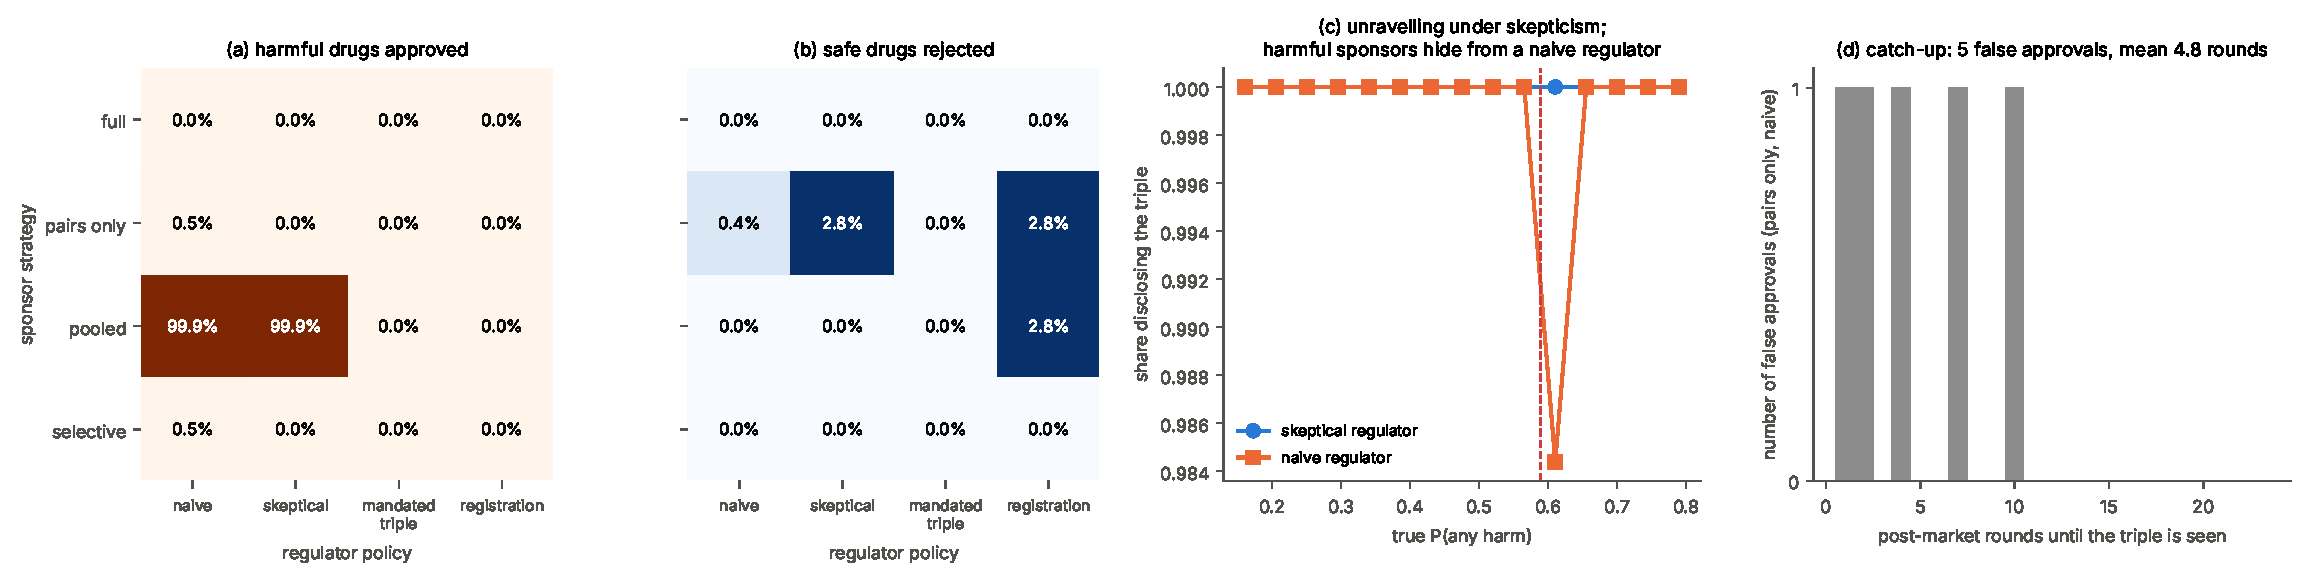
\includegraphics[width=\linewidth]{fig_game.pdf}
\caption{The disclosure game. (a, b) Error rates by sponsor strategy and regulator policy. (c) Unravelling: under a skeptical regulator
every sponsor discloses (ties included), while a naive regulator lets harmful sponsors hide. (d) After a false approval, post-market
use reveals the triple with probability $0.2$ per round.}\label{fig:game}
\end{figure}

\begin{figure}[!htbp]\centering
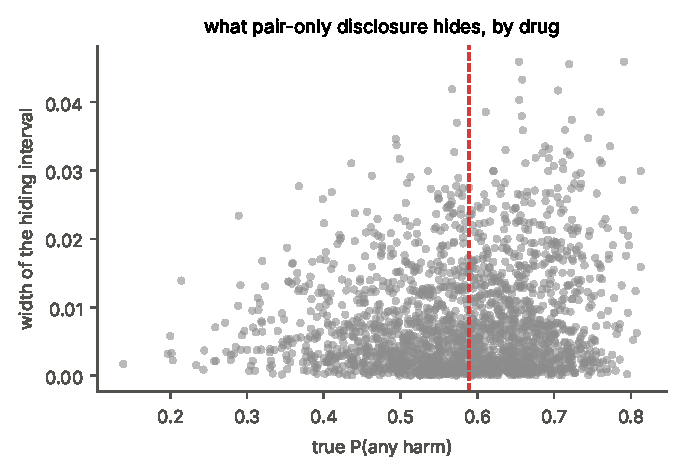
\includegraphics[width=0.48\linewidth]{fig_hiding.pdf}
\caption{What pair-only disclosure hides, drug by drug: the width of the interval for the triple's harm.}\label{fig:hiding}
\end{figure}

\section{For machine learning: RL and adversarial training}\label{sec:ml}
\begin{itemize}
\item \emph{RL.} The lab is a partially observed decision process \cite{KaelblingLittmanCassandra1998}. The actors are the hidden state,
  and the probe is an information-gathering action, as in Bayesian and sequential optimal experimental design
  \cite{Lindley1956,ChalonerVerdinelli1995,ShenDongHuan2023}. \Cref{thm:B} gives the sample complexity in closed form: rate $0$, $n^{-1/2}$
  or $n^{-1/4}$ depending on the stratum. \Cref{thm:C}(5) gives the optimal probe in closed form, and \cref{thm:D}(4) gives the sample complexity of the decision itself,
  $n^*=(z\tau/d)^2$, which is not the same as that of the estimate.
  The nearest hardness result is for \emph{partial online state information} (POSI) \cite{ShiLiangShroff2023}: a learner that can query
  only some components of the latent state at each step may need $\Omega(A^{H-1}/\varepsilon^2)$ episodes to find an
  $\varepsilon$-optimal policy (exponential in the horizon $H$, with $A$ actions), while two structured subclasses are learnable with
  regret $\tilde O(\sqrt K)$ over $K$ episodes. The lab is a one-step analogue with a different query: the type is never revealed, and a
  probe returns a marginal table on a window. The segment's geometry plays the role of their structural assumptions; it is what turns
  the probe choice into the closed-form rule of \cref{thm:C}(5).
\item \emph{Adversarial training.} The sponsor--regulator interaction is a minimax game, like a GAN's generator and discriminator
  \cite{Goodfellow2014}. It shares their dynamics: simultaneous gradient play rotates around a mixed equilibrium and need not converge
  \cite{Mescheder2018}, while commitment by one side converges. Divergence choice matters as in $f$-GANs
  \cite{Nowozin2016}. Here the worst case over the segment plays the role of the discriminator's objective.
\end{itemize}
\Cref{fig:ml} shows two illustrations; they illustrate the analogy and are not evidence for the theorems.
\begin{itemize}
\item A contextual bandit, given $|\hat v_S|$ as a feature, learns to choose probes. After 3000 episodes it reaches $99.7\%$ of the
  closed-form rule's value, far above random choice.
\item In a stylised inspection game between regulator and sponsor, the registered illustration I2 predicted that simultaneous gradient play
  would not approach the mixed equilibrium (final distance at least the initial one). It failed as registered: the distance falls from
  $0.83$ to $0.33$. Post hoc, play then stays on a persistent cycle at distance $0.26$--$0.34$ and never converges, the rotation that
  \cite{Mescheder2018} describes. With the regulator committing first, as
  pre-registration does, play converges to honesty.
\end{itemize}

\begin{figure}[!htbp]\centering
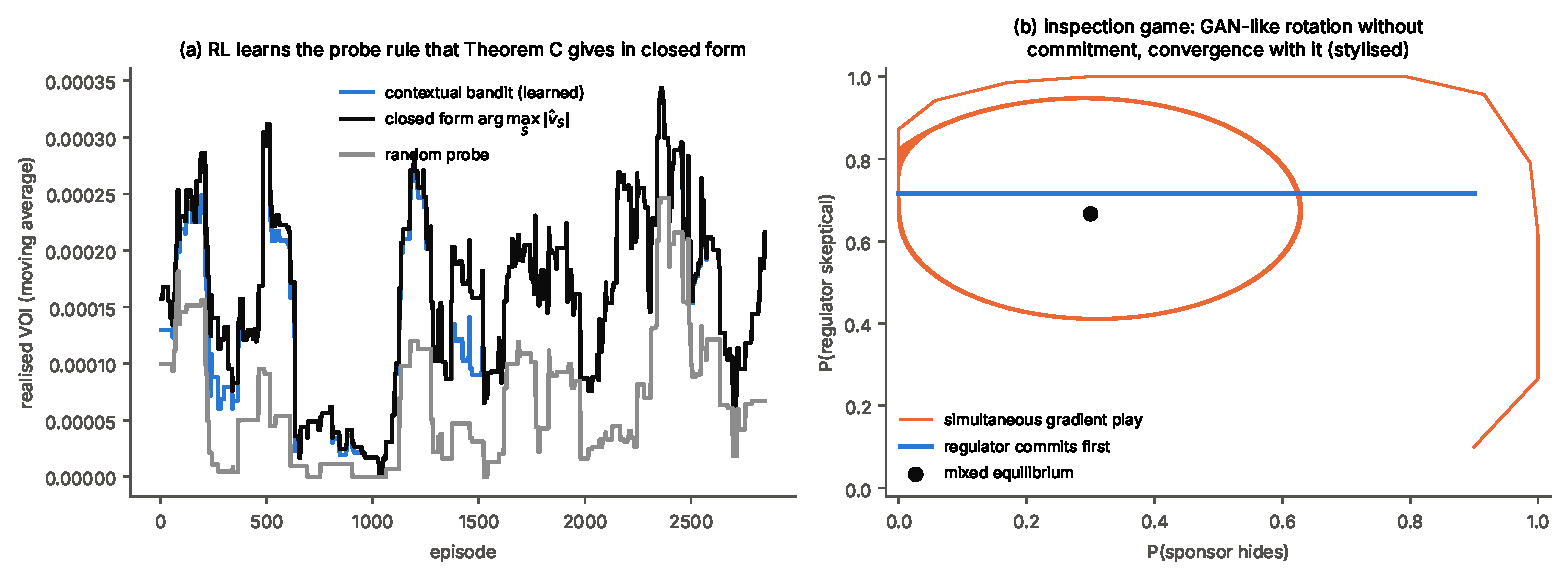
\includegraphics[width=\linewidth]{fig_ml.pdf}
\caption{(a) A bandit learns the probe rule that \cref{thm:C} states in closed form. (b) Inspection-game dynamics: rotation without
commitment, convergence with it (stylised).}\label{fig:ml}
\end{figure}

\section{Part II. Injected records: actors who feed the data}\label{sec:inj}
Part I asked what a regulator can learn when an interested party chooses which tables to reveal. Part II asks what happens when that
party \emph{adds records}: data written to tilt the decision. We study whole-record injection only. The adversary adds complete
records, so every window is a marginal of one law.

\paragraph{The model.} Genuine records follow the two-type law $P$. The adversary adds records drawn from a law $Q$ of its choice, a
share $\varepsilon$ of the data. Within the injected set any dependence is allowed, since $Q$ is arbitrary; between injected and genuine
records there is none. The dataset is therefore a disjoint union, a coproduct of two samples, and every window sees the marginal of
\[
P_\varepsilon=(1-\varepsilon)P+\varepsilon Q .
\]
This is Huber's contamination model \cite{Huber1964} with intent behind it, and the level-one contamination model of \cite{PG} read
adversarially. It is narrower than editing genuine records, where the reachable set is a whole total-variation ball.

\paragraph{A categorical framing.} Provenance is a context the regulator cannot see. Formally it is the environment comonad
$W=E\times(-)$ on sets of records, with $E=\{\text{genuine},\text{injected}\}$. The counit $W X\to X$ forgets provenance, and it is
exactly what the regulator observes. The comultiplication copies the label. A $W$-coalgebra on $X$ is a labelling $X\to E$. ``No relation
between the two sets'' says the dataset is the coproduct $X_g\sqcup X_a$; pushed forward to window tables, a coproduct becomes a
mixture. Every procedure the regulator can run factors through the counit. The framing names the situation precisely, but the results
below come from three other structures: the polytope of reachable laws, the Walsh characters of $\{0,1\}^m$, and the scheme cut out by
the model's equations.

\section{Theorem E: slopes and the vertex attack}\label{sec:E}
Let $F=(F_j)$ be decision statistics: smooth functions of the window tables such that the regulator's act is unchanged while every
$F_j>0$. An example is the set-rule constraints of \cref{thm:D}. Write $\mathrm{IF}_j(x)=\frac{d}{d\varepsilon}F_j\bigl(P+\varepsilon(\delta_x-P)\bigr)|_0$,
Hampel's influence function \cite{Hampel1974} of a single injected record $x$.

\begin{theorem}[slopes and the vertex attack]\label{thm:E}
\begin{enumerate}
\item[(1)] \emph{Reachable set.} At budget $\varepsilon$ the reachable laws form the polytope $(1-\varepsilon)P+\varepsilon\Delta$, with
vertices $(1-\varepsilon)P+\varepsilon\delta_x$. Every window table is a marginal of the one law $P_\varepsilon$, so whole-record
injection never makes the windows fail to glue ($\lambda^*=1$).
\item[(2)] \emph{Slopes are linear in the injected law:} $\frac{d}{d\varepsilon}F_j(P_\varepsilon)|_0=\sum_xQ(x)\,\mathrm{IF}_j(x)$.
\item[(3)] \emph{The vertex attack.} To first order the smallest budget that changes the act is
\[
\varepsilon^*_1=\min_{j,\,x:\ \mathrm{IF}_j(x)<0}\ \frac{F_j(P)}{-\mathrm{IF}_j(x)},
\]
attained by a point mass: copies of one record. The exact smallest budget is
$\varepsilon^*_1\,\bigl(1+O(\min_jF_j(P))\bigr)$.
\item[(4)] \emph{The injected set is a latent actor.} If $Q$ is a product law, $P_\varepsilon$ is a three-type law with weights
$(1-\varepsilon)w$, $(1-\varepsilon)(1-w)$ and $\varepsilon$. Its pair covariances are $(1-\varepsilon)vv^\top+\varepsilon(1-\varepsilon)\Delta\Delta^\top$
off the diagonal, with $\Delta=\mu_P-\mu_Q$. They stay rank one exactly when $\Delta$ is parallel to $v$: the injected actor then
imitates the latent axis.
\end{enumerate}
\end{theorem}

\begin{proof}
(1) $P_\varepsilon$ is affine in $Q$, and $Q$ ranges over the simplex. (2) The chain rule, with $\sum_xQ(x)(\delta_x-P)=Q-P$.
(3) To first order $F_j(P_\varepsilon)=F_j(P)+\varepsilon\sum_xQ(x)\mathrm{IF}_j(x)$, and a linear function on the simplex is smallest
at a vertex. The second-order remainder is $O(\varepsilon^2)$, and $\varepsilon^*=O(\min_jF_j)$, so the relative error is
$O(\min_jF_j)$. (4) A mixture's covariance is the weighted within-component covariance plus the between-component term, and a product
law has none of its own.
\end{proof}

Part (3) is the first-order energy shift of perturbation theory: the decision's margin divided by the steepest single-record influence.
At a tie (the stratum $d=0$ of \cref{thm:D}) the margin is zero, and an arbitrarily small injection decides the act. Which act wins is
then set by the sign of the influence difference, as in degenerate perturbation theory. Check IN3 shows the exact budget of the best
point mass approaching $\varepsilon^*_1$ as the margin shrinks, and no random injected law beating it.

\section{Theorem F: the hidden channel}\label{sec:F}
Write $\chi_S(x)=\prod_{i\in S}(2x_i-1)$.

\begin{theorem}[the hidden channel]\label{thm:F}
Let $m=3$ and $T=\{0,1,2\}$.
\begin{enumerate}
\item[(1)] The injected laws that leave every single and pair table unchanged are exactly $Q=P+s\chi_T$, with
$s\in[s_-,s_+]=[\max_{\chi_T(x)>0}(-P(x)),\ \min_{\chi_T(x)<0}P(x)]$. They form a segment: the adversary's own hiding segment.
\item[(2)] Injecting them leaves $\mu$, $v$, the regulator's segment $R$ and the pre-probe act unchanged, and moves the estimate of $r$
by exactly
\[
\hat r(P_\varepsilon)=r_0+\varepsilon s/v_T .
\]
\item[(3)] Let $r_c$ be the nearest point beyond which the oracle act changes, on the side $\operatorname{sign}(s/v_T)$, and let $|s|$ be
the positivity limit on that side. With exact tables, the act switches at $\varepsilon^*=|r_c-r_0|\,|v_T|/|s|$, and the triple
contradicts the pairs ($\hat r\notin R$) only at $\varepsilon_{\det}=|w-r_0|\,|v_T|/|s|$, where $w$ is the wall on that side. Since $r_c$
lies inside $R$, $\varepsilon^*<\varepsilon_{\det}$: there is always a \emph{stealth window} in which the decision is taken over and
nothing is flagged. With $n$ records per window and one binding constraint, the share choosing the oracle act crosses one half at
$\varepsilon_{1/2}=\bigl(|r_c-r_0|-\kappa z\tau/\sqrt n\bigr)|v_T|/|s|$, where $\kappa=\gamma_j/|g_j'|$ is $1$ for a flat competitor.
\item[(4)] For general $m$ and a triple $S$, $Q=P+s\chi_S$ leaves every single and pair table and every other triple moment unchanged,
and moves $\hat r_S$ by $2^{m-3}\varepsilon s/v_S$. The budget is therefore proportional to $|v_S|$: the factor that makes $S$ the best
probe (\cref{thm:C}(5)) and sets its tempo (\cref{thm:B}) also makes it the hardest to poison.
\end{enumerate}
\end{theorem}

\begin{proof}
(1) On $\{0,1\}^3$ the singles, pairs and total mass are 7 linear functionals of rank 7, so their kernel is one-dimensional. The
characters are orthogonal, and $\chi_T$ is orthogonal to every character of order at most two, so it spans the kernel. Positivity of
$Q$ gives the bounds. (2) The means are unchanged, so central moments are linear in the law, and
$m_T(P_\varepsilon)=m_T(P)+\varepsilon s\sum_x\chi_T(x)\prod_{i\in T}(x_i-\mu_i)$. The sum factorises as
$\prod_{i}\bigl((1-\mu_i)+\mu_i\bigr)=1$. The pair tables give $v$ and $R$ (\cref{thm:A}), and they are unchanged. (3) follows from (2)
and, at finite $n$, from \cref{thm:D}(4) with the constraint evaluated at the shifted point. (4) The same factorisation over $S$, with a
factor $\sum_{x_i}1=2$ for each $i\notin S$; for any set $S'$ with $S'\not\supseteq S$ a factor $\sum_{x_i}(2x_i-1)=0$ appears.
\end{proof}

\begin{corollary}[capacity of the channel]\label{cor:capacity}
The hidden channel of a triple $S$ has capacities
\[
\mathrm{cap}_+(S)=s_+=\min_{\chi_S(x)<0}P(x),\qquad \mathrm{cap}_-(S)=-s_-=\min_{\chi_S(x)>0}P(x),
\]
one for each direction: the probability of the rarest outcome that the injection must drain. On the side where the adversary needs
$\operatorname{sign}(s/v_S)$, the flip budget is
\[
\varepsilon^*(S)=\frac{|r_c-r_0|\,|v_S|}{2^{m-3}\,\mathrm{cap}(S)} ,
\]
and the detection budget is the same expression with the distance to the wall. A probe whose rarest joint outcomes are rarer leaves the
adversary less room. Among triples, the regulator should prefer those with large $|v_S|/\mathrm{cap}(S)$; this is the poisoning
counterpart of the probe rule $\arg\max_S|v_S|/\sigma_S$ of \cref{thm:C}(5).
\end{corollary}

\begin{proof}
$Q=P+s\chi_S$ is a law iff $P(x)+s\chi_S(x)\ge0$ for all $x$. For $s>0$ only the cells with $\chi_S=-1$ can reach zero, which gives
$s\le\min_{\chi_S<0}P(x)$, and symmetrically for $s<0$. The budgets follow from \cref{thm:F}(3) and (4), with the shift
$2^{m-3}\varepsilon s/v_S$.
\end{proof}

On Study 11's four-variable truth G the two rules agree. The best probe, $\{0,1,2\}$, has the largest $|v_S|/\sigma_S$ ($0.097$) and the
smallest largest shift per unit of injected share ($4.61$ in $r$); the order of the four triples is the same under both rules:
$\{0,1,2\}$, $\{0,2,3\}$, $\{1,2,3\}$, $\{0,1,3\}$, with shifts $4.61$, $5.94$, $7.75$ and $10.85$ (check IN14).

\section{Theorem G: stealth when there are equations}\label{sec:G}
With three variables the model has no equations on the pair tables, only inequalities, so any injection into pairs is invisible
except through an empty fibre. With four variables there are two, the tetrads $T_1=M_{01}M_{23}-M_{02}M_{13}$ and
$T_2=M_{01}M_{23}-M_{03}M_{12}$: the off-diagonal pair covariances have rank one \cite{DrtonSturmfelsSullivant2007}. Let
$N(Q)=\sum_xQ(x)\nabla T(x)$ be the tetrads' first-order response, the tetrad Jacobian applied to $Q$.

\begin{theorem}[stealth with equations]\label{thm:G}
Let $m=4$.
\begin{enumerate}
\item[(1)] \emph{Tangent stealth.} The tetrads move by $\varepsilon N(Q)+O(\varepsilon^2)$. An injection with $N(Q)=0$ is a point of the
scheme $\operatorname{Spec}\R[M]/(T_1,T_2)$ over the dual numbers $\R[\varepsilon]/(\varepsilon^2)$, based at $P$: it is invisible to
first order: a straight injection moves the tetrads only at order $\varepsilon^2$, so a Wald test of the tetrads has noncentrality of
order $n\varepsilon^4$ rather than $n\varepsilon^2$.
\item[(2)] \emph{The stealth--tilt frontier.} For a tilt functional with influence $\mathrm{IF}$ and whitened Jacobian $N_w$,
$\Phi(\delta)=\max\{\sum_xQ(x)\mathrm{IF}(x):Q\in\Delta,\ |N_w(Q-P)|_\infty\le\delta\}$ is concave and piecewise linear in $\delta$. With
$n_x\in\R^2$ the whitened tetrad response to one injected record $x$, it has the closed form
\[
\Phi(\delta)=\min_{\lambda\in\R^2}\Bigl[\max_x\bigl(\mathrm{IF}(x)-\lambda^\top n_x\bigr)+\delta\,\|\lambda\|_1\Bigr],
\]
a minimum of finitely many affine functions of $\delta$. An optimal injection mixes at most three records. $\Phi$ rises from the best
invisible tilt $\Phi(0)$ to the vertex tilt $\max_x\mathrm{IF}(x)$, which it reaches at $\bar\delta=\|n_{x^*}\|_\infty$ for the best
record $x^*$.
\item[(3)] \emph{Strata.} The tetrad Jacobian has rank $2$ at a generic truth and at a single coincidence ($v_i=0$), rank $1$ when two
coordinates of $v$ vanish, and rank $0$ at the merge ($v=0$). So the space of first-order stealthy injections grows on the strata,
which are also where Part I's hiding happens.
\item[(4)] \emph{Obstruction.} The model's ring $A=\R[M]/(T_1,T_2)$ is commutative, so the obstruction to extending a first-order
stealthy injection to second order is an André--Quillen class, in $\operatorname{Ext}^1_A(L_{A/\R},\kappa(P))$ \cite{Quillen1970,Andre1974}.
Where the tetrads form a regular sequence it is explicit: for a first-order stealthy direction $A$ ($JA=0$, with $J$ the tetrads'
Jacobian and $H$ their second derivative at $P$),
\[
\mathrm{ob}(A)=\bigl[\tfrac12H(A,A)\bigr]\in\operatorname{coker}J ,
\]
and $A$ extends to a second-order stealthy injection iff $\mathrm{ob}(A)=0$. Hence:
\begin{itemize}
\item Where $J$ has rank 2 (generic truths, single coincidences) the cokernel is $0$, every $A$ extends, and an adversary that bends its
  injection, letting $Q$ depend on $\varepsilon$, keeps the tetrads still to third order.
\item On the two-coincidence stratum, say $v_2=v_3=0$, the cokernel is the line spanned by $T_1-T_2$ and
  $\mathrm{ob}(A)=q(A)=dM_{03}\,dM_{12}-dM_{02}\,dM_{13}$ evaluated on $A$. It vanishes exactly on the quadric cone $\{q=0\}\cap\ker J$, so
  a generic stealthy direction is obstructed and moves the tetrads at order $\varepsilon^2$ along every bent injection.
\item At the merge $J=0$, the cokernel is all of $\R^2$, and $\mathrm{ob}(A)=\tfrac12H(A,A)$ itself.
\end{itemize}
A non-zero cokernel is necessary for an obstruction but not sufficient: the class can vanish on special directions. So the strata give
more first-order stealth but obstructed second-order stealth.
\end{enumerate}
\end{theorem}

\begin{proof}
(1) Taylor expansion. A $\R[\varepsilon]/(\varepsilon^2)$-point based at $P$ is a tangent vector annihilated by the Jacobian of the
defining equations. The noncentrality is $n\,T(P_\varepsilon)^\top\Sigma_T^{-1}T(P_\varepsilon)$ with $T(P_\varepsilon)=O(\varepsilon^2)$.
(2) Since $\sum_xQ(x)(\delta_x-P)=Q-P$, the constraint is $|\sum_xQ(x)n_x|_\infty\le\delta$: a linear programme in $Q$ with one equality
($\sum Q=1$), four inequalities and $16$ non-negative variables. Its dual has a free multiplier $\lambda=\lambda^+-\lambda^-$ for the four
inequalities and one for the equality, and it is the displayed minimum; strong duality holds because $Q=P$ is feasible. The value is a
minimum of affine functions of $\delta$, one per dual vertex, so it is concave and piecewise linear. A basic optimal solution has at most
as many non-zero coordinates as active constraints, the equality and at most two of the tetrad bounds, hence at most three records. For
$\delta\ge\|n_{x^*}\|_\infty$ the point mass at $x^*$ is feasible and optimal. (3) The covariances respond to the law surjectively, so the rank is that of $\partial T/\partial M$. With $M_{ij}=v_iv_j$ and,
for example, $v_3=0$, the rows are $M_{01}\,dM_{23}-M_{02}\,dM_{13}$ and $M_{01}\,dM_{23}-M_{12}\,dM_{03}$, which are independent. With
$v_2=v_3=0$ both rows equal $M_{01}\,dM_{23}$, and $v=0$ kills both. Check IN8 confirms every single and every pair of coincidences.
(4) A bent injection $P+\varepsilon A+\varepsilon^2B$ with $JA=0$ keeps the tetrads to third order iff $JB=-\tfrac12H(A,A)$ is
solvable, where $H$ is their second derivative; the class of $\tfrac12H(A,A)$ in $\operatorname{coker}J$ is the obstruction. For a
presentation by a regular sequence, the cotangent complex is the two-term complex $I/I^2\to\Omega_{\R[M]}\otimes A$, and
$\operatorname{Ext}^1(L_{A/\R},\kappa(P))$ is that cokernel. If $J$ is surjective the cokernel is zero. On the two-coincidence stratum
both rows of $J$ are $M_{01}\,dM_{23}$, so its image is the diagonal of $\R^2$ and the cokernel is detected by $T_1-T_2$. The quadratic
part of $T_1-T_2=M_{03}M_{12}-M_{02}M_{13}$ at a point where these four covariances vanish is $dM_{03}\,dM_{12}-dM_{02}\,dM_{13}$, a
non-degenerate quadratic form in four of the free directions of $\ker J$; its zero set there is a quadric cone, and off it the class is
non-zero (check IN11 finds it non-zero on random stealthy directions). At the merge every covariance vanishes, $J=0$ and nothing is
quotiented.
\end{proof}

On the H4 truth of Study 12 the frontier has three pieces: $\Phi(\delta)=10.144+0.417\,\delta$ up to $\delta=0.219$, then slope
$0.201$ up to $\bar\delta=2.744$, where it reaches the vertex tilt $10.743$ and stays. The optimal injection mixes three records at
$\delta=0$ ($1100$, $1101$ and $0111$), two on the middle piece, and one, the point mass at $1101$, from $\bar\delta$ on (check IN13).

The $\varepsilon^2$ movement of a straight stealthy injection in (1) is curvature, not obstruction: at smooth points bending removes it.
The obstruction proper is (4), and it is André--Quillen rather than Hochschild because the ring is commutative. Hochschild cohomology
governs the noncommutative observable algebras of \cite[Section~15]{PG}, and the Hochschild--Kostant--Rosenberg theorem ties the two
theories only at smooth points, while the obstruction lives exactly at the singular ones. On random truths a straight stealthy injection
moves the tetrads with log--log slope $1.99$, against $0.98$ for a vertex attack. A bent one moves them with slope $3.0$ at a generic
truth and $2.0$ on the two-coincidence stratum.

\section{Theorem H: one geometry for the regulator and the adversary}\label{sec:H}
Fix the pair tables of $P$. Let $\Pi$ be the set of all laws with these pair tables, the \emph{pair fibre}, and let $X\subseteq\Pi$ be
the regulator's hiding segment, the two-type explanations.

\begin{theorem}[one geometry]\label{thm:H}
\begin{enumerate}
\item[(1)] \emph{One line} ($m=3$). $\Pi=\{P+s\chi_T\}\cap\Delta$ is a segment, and $X$ is a sub-segment of it, strictly inside it
unless both types meet a wall at once. In the triple-moment coordinate, $X$ is $v_T\cdot R$ and $\Pi$ is $m_T(P)+[s_-,s_+]$. The
regulator reads this line in units of $v_T$, since $r=m_T/v_T$; the adversary moves along it by $\varepsilon s$. The two segments are the
model's part and the positivity part of one line, and that is why $1/v_T$ governs the value of a probe (\cref{thm:C}), its tempo
(\cref{thm:B}) and its vulnerability (\cref{thm:F}) alike.
\item[(2)] \emph{One geometry} ($m=4$). $\Pi$ has dimension 5. The directions in $\Pi$ that preserve every equation of the model to
first order form a line: the tangent of $X$. Those equations are the equality of $r_S=m_S/v_S$ across the four triples, and
$m_{0123}=v_{0123}(r^2+1)$; the tetrads are constant on $\Pi$. So an injection invisible to every equation of the model moves the
observed law along the regulator's own hiding segment. A single-triple channel $\chi_S$ moves $r_S$ alone, and a second triple sees it at
first order.
\end{enumerate}
\end{theorem}

\begin{proof}
(1) Given the singles and pairs, the law of three binary variables is affine in $m_T$, which is \cref{thm:F}(1). The two-type laws with
these pairs are those with $m_T=v_Tr$, $r\in R$. They are laws, so $X\subseteq\Pi$. The two segments end for different reasons. $\Pi$ ends
where some cell of $P+s\chi_T$ reaches $0$. $X$ ends at a box wall, where one type's harm probability on one variable reaches $0$ or $1$.
At such a wall, say $a_{1i}=0$, the first type gives no mass to the cells with $x_i=1$. But each cell is
$P(x)=w_1\prod_j a_{1j}^{x_j}(1-a_{1j})^{1-x_j}+w_2\prod_j a_{2j}^{x_j}(1-a_{2j})^{1-x_j}$, and the second term is positive whenever
$w_2>0$ and every $a_{2j}$ lies strictly inside $(0,1)$. So every cell is still positive, the positivity bound is not reached, and the
end of $X$ lies strictly inside $\Pi$. Equality is possible only if the second type is at a wall too, so that some cell receives no mass
from either type. In the worked example (\cref{sec:example}) the smallest cell is $0.0152$ at one wall and $0.0068$ at the other, both positive. (2) $\dim\Pi=16-1-4-6=5$. Given the pairs, the model fixes the four triple moments and the quadruple moment up to the single
parameter $r$: four constraints on five coordinates, with Jacobian of rank 4 when no $v_i$ vanishes. The kernel is one-dimensional and
contains the tangent of $X$. A channel $\chi_S$ moves $m_S$ alone (\cref{thm:F}(4)), so it changes $r_S$ and not $r_{S'}$.
\end{proof}

\begin{corollary}[the second-triple defence]\label{cor:secondtriple}
Let $m=4$ and let $S\neq S'$ be triples with $v_S,v_{S'}\neq0$.
\begin{enumerate}
\item[(a)] The single-triple channel $Q=P+s\chi_S$ moves $\hat r_S$ by $2\varepsilon s/v_S$ and leaves $\hat r_{S'}$ unchanged, so the
  difference $\hat r_S-\hat r_{S'}$, which is $0$ under the model, moves at first order. Any second triple catches it, with the noise
  of a difference of two estimates (\cref{thm:B}).
\item[(b)] An injection that no second triple, no tetrad and no quadruple moment can see to first order must move all four $r_S$
  together and $m_{0123}$ consistently with them: it moves the observed law along the regulator's hiding segment (\cref{thm:H}(2)). Its
  room is then the distance to the segment's walls, as at $m=3$.
\end{enumerate}
\end{corollary}

\begin{proof}
(a) is \cref{thm:F}(4) together with $r_S=r_{S'}=r$ under the model. (b) is \cref{thm:H}(2).
\end{proof}

As a check, take the truth with weights $(0.35,0.65)$, $a_1=(0.8,0.3,0.7,0.25)$ and $a_2=(0.2,0.7,0.15,0.7)$, where all four $r_S$
equal $0.629$. Injecting $5\%$ of records from $P+s\chi_{\{0,1,2\}}$, with $s$ half its capacity ($0.0137$), moves $\hat r_{\{0,1,2\}}$ to
$0.533$, exactly the predicted shift $2\varepsilon s/v_S=-0.096$, while the other three stay at $0.629$ (check IN12).

\begin{proposition}[two boundaries of one geometry]\label{prop:twoboundaries}
On the line of \cref{thm:H}(1) mark the truth $r_0$, the \emph{decision boundary} $r_c$ where the oracle act changes, and the
\emph{detection boundary}, the walls of $R$. The regulator's margin is the distance from $r_0$ to the decision boundary (the
post-probe form of \cref{thm:D}(3)). The adversary's room is the distance from $r_0$ to the detection boundary. A stealthy takeover is
possible on a side exactly when the decision boundary is nearer, which holds whenever $r_c\in R$. At $m=4$ the detection boundary
becomes the stealth--tilt frontier of \cref{thm:G}(2) together with the model equations of \cref{thm:H}(2).
\end{proposition}

\begin{proof}
\Cref{thm:F}(3), read on the line of \cref{thm:H}(1).
\end{proof}

The decision lab and the adversarial lab are therefore one lab. Part I measures the distance to the boundary where the act changes;
Part II measures the distance to the boundary where the change becomes visible. Both are read on the same stratified fibre, and both
scale with the same $v_T$. Checks IN1--IN14 verify Theorems E--H and their corollaries.

\begin{figure}[!htbp]\centering
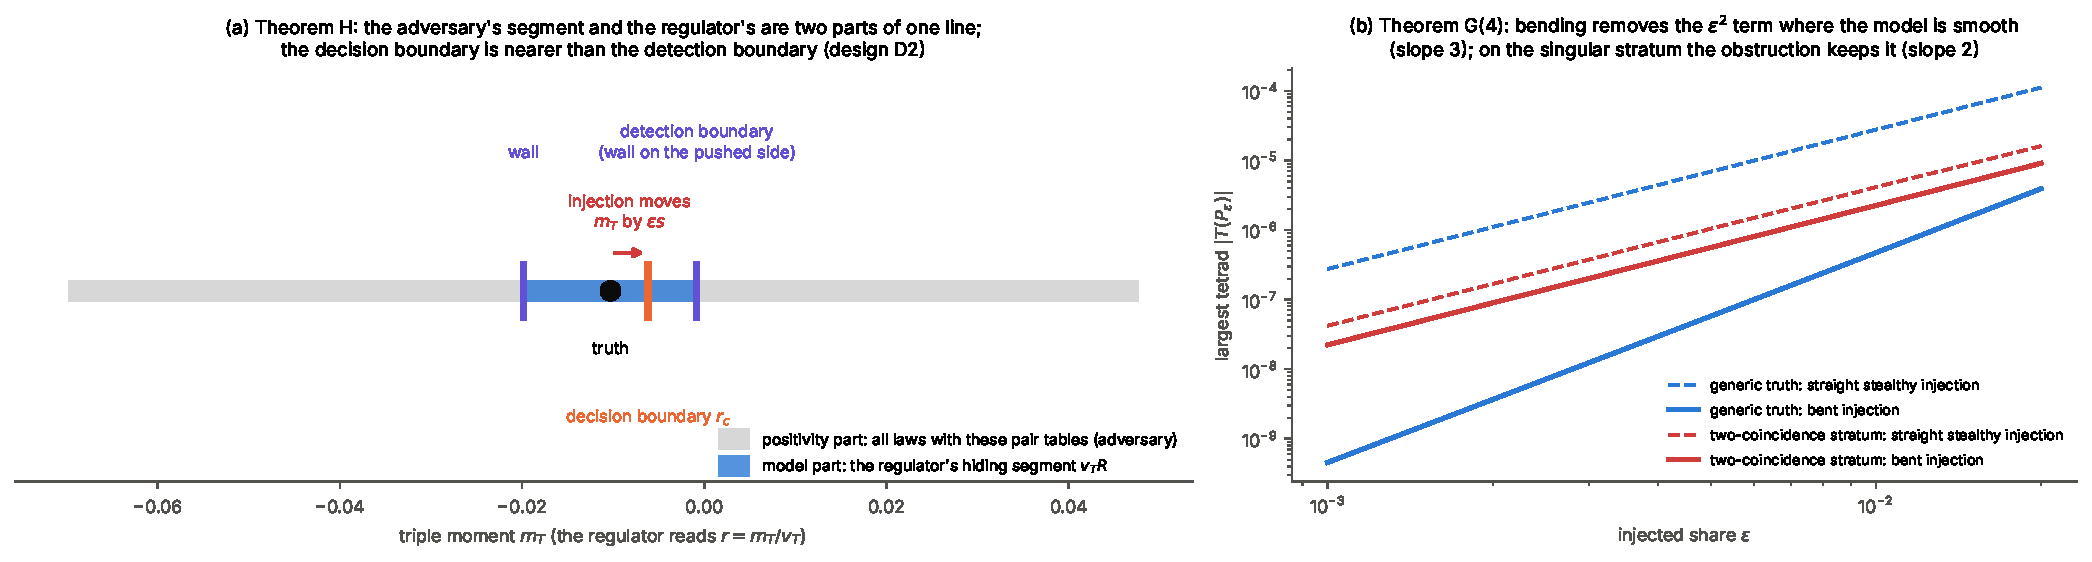
\includegraphics[width=\linewidth]{fig_oneline.pdf}
\caption{(a) \Cref{thm:H} and \cref{prop:twoboundaries} on design D2, in the triple-moment coordinate. All laws with the observed pair
tables form the grey segment; the regulator's hiding segment is the blue part of it. The injection walks the truth to the decision
boundary well before the detection boundary. (b) \Cref{thm:G}(4): tetrads against the injected share. A straight stealthy injection
moves them at order $\varepsilon^2$. Bending removes that term at a smooth point (slope 3) but not on the singular stratum (slope 2),
where the André--Quillen obstruction is non-zero.}\label{fig:oneline}
\end{figure}

\section{Study 12: injection in practice}\label{sec:study12}
Study 12 was registered and frozen before any registered design was simulated
(\texttt{engine/\allowbreak study12\_inject/\allowbreak PREREG\_study12.md}).
One irregularity is disclosed in the registration. The smoke run's tetrad part used the $m=4$ truth then intended for H4. That truth was
demoted, and H4 moved to a fresh truth before freezing; the criteria were fixed in code before the smoke run and were not changed.

There are two designs.
\begin{itemize}
\item \emph{H1--H3: the hidden channel.} Design D2 of Study 11b, with $Q=P+s\chi_T$ at the positivity limit $s=0.058$ and
  $n=10^5$ records per window. The theory gives $\varepsilon_{1/2}=0.058$ (closed form; $0.059$ from the delta-method curve),
  $\varepsilon^*=0.071$ and $\varepsilon_{\det}=0.164$.
\item \emph{H4: first-order stealth at $m=4$.} A Wald test of the tetrads at level $0.05$. Two injections have the same first-order
  tilt of $\hat r$ ($0.3$): the best tetrad-blind law from the linear programme, and a point mass.
\end{itemize}

\begin{table}[!htbp]\centering\small
\begin{tabular}{p{0.06\linewidth}p{0.6\linewidth}p{0.26\linewidth}}\toprule
& prediction & outcome\\\midrule
H1 & share choosing the genuine act within $0.05$ of prediction ($\ge9$ of 10 cells); half-way point within $10\%$ & holds: 10 of 10, largest gap $0.012$; $0.0581$ vs $0.0587$\\
H2 & flag rate within $0.05$ ($\ge6$ of 7); half-way point within $5\%$ of $\varepsilon_{\det}$ & holds: largest gap $0.005$; $0.1636$ vs $0.1635$\\
H3 & at $\varepsilon=0.07$ the decision is taken over ($\le0.5$) and at most $1\%$ is flagged & holds: $0.31$ and $0$\\
H4 & tetrad-test rejection within $0.04$ of the noncentral-$\chi^2$ prediction ($\ge5$ of 6); stealth $\le0.10$ at every $n$; vertex $\ge0.80$ at $n=50000$ & holds: largest gap $0.016$; stealth $0.045$--$0.048$; vertex $0.84$, $1.00$, $1.00$\\\bottomrule
\end{tabular}
\caption{Study 12: registered predictions and outcomes.}\label{tab:study12}
\end{table}

All four held (\cref{tab:study12,fig:inject}). Injecting about $6\%$ of records into the mandated triple, records that leave every pair
rate unchanged, takes the decision over half the time. At $7\%$ it is taken over $69\%$ of the time, and not one replicate in 4000 is
flagged. Detection begins only near $15\%$. At $m=4$ the tetrad-blind injection costs about $6\%$ of the tilt and stays at the test's
level at every sample size, while the point mass with the same tilt is rejected $84\%$ of the time already at $n=2000$.

\begin{figure}[!htbp]\centering
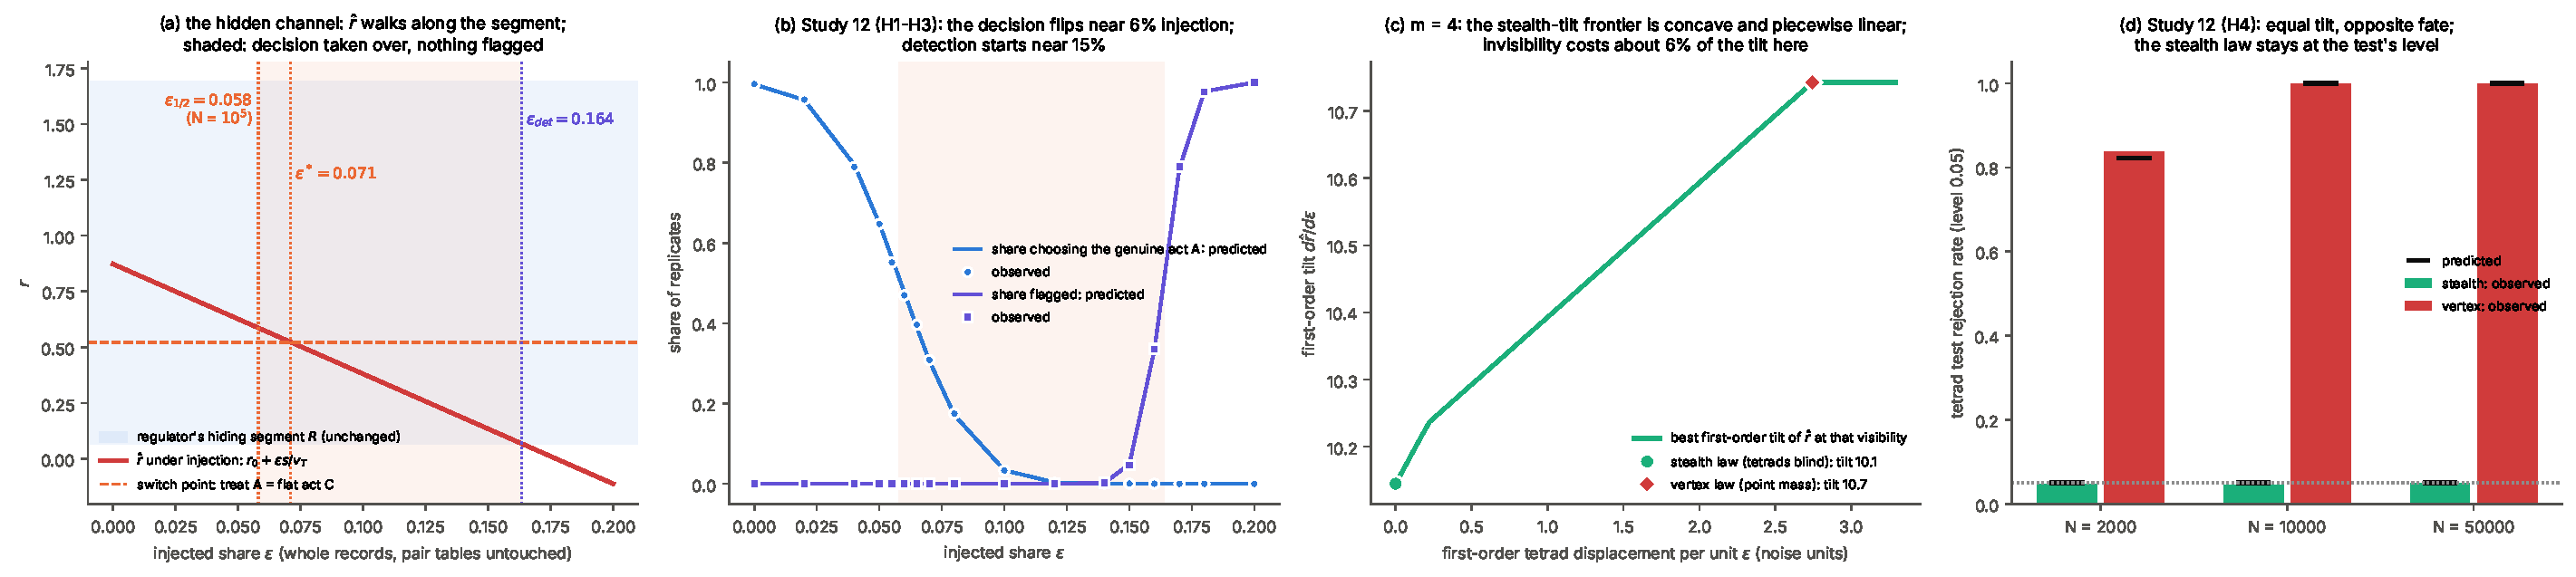
\includegraphics[width=\linewidth]{fig_inject.pdf}
\caption{Part II. (a) The hidden channel on design D2: the estimate of $r$ walks along the regulator's segment as the injected share
grows, while the segment itself does not move. The decision is taken over between $\varepsilon_{1/2}$ and $\varepsilon_{\det}$ with
nothing flagged (shaded). (b) Study 12, H1--H3: share choosing the genuine act and share flagged, predicted (lines) and observed. (c) The
stealth--tilt frontier at $m=4$ (\cref{thm:G}(2)); the vertical axis is zoomed. (d) Study 12, H4: tetrad-test rejection for injections
of equal tilt.}\label{fig:inject}
\end{figure}

\paragraph{For the three readerships.}
\begin{itemize}
\item \emph{Decisions.} A satisficing margin has a price in injected records, $\varepsilon^*_1$ (\cref{thm:E}). Against the hidden
  channel the price is $|r_c-r_0|\,|v_T|/|s|$ (\cref{thm:F}), and no consistency check on the tables can raise it.
\item \emph{Persuasion and disclosure.} Mandating the triple (\cref{cor:unravel}) opens the channel through which a sponsor who runs it
  can tilt it. The channel moves joint outcomes without changing any pair rate, so it is invisible to everything Part I's regulator
  checks. Defences are a second triple, which sees a single channel at first order (\cref{thm:H}(2)); patient-level audit; or four or more
  variables, where every model-invisible injection must move along the hiding segment itself.
\item \emph{Machine learning.} This is data poisoning \cite{BiggioNelsonLaskov2012} in a model small enough to solve. The vertex attack
  is the optimal single-point poison. $\varepsilon^*$ is a certified budget for this pipeline, in the spirit of
  \cite{SteinhardtKohLiang2017}, and the stealth--tilt frontier is the trade-off that robust high-dimensional estimators
  \cite{DiakonikolasEtAl2019} are built to cut.
\end{itemize}

\section{A worked example, end to end}\label{sec:example}
This section carries one example through every step of the paper, with enough arithmetic that each number can be checked by hand. The
truth is population~1 of the main note's drug example \cite[Example ``conflicting pair trials'']{PG}: two patient types with weights
$(0.6,0.4)$ and harm probabilities $a_1=(0.5,0.1,0.4)$ and $a_2=(0.05,0.5,0.1)$ for the harms $A$, $B$, $C$ of three drugs. The script
\texttt{engine/worked\_example.py} recomputes every number below and asserts the hand checks (WE0--WE18). \Cref{tab:example} collects
the numbers, and \cref{fig:worked} draws them.

\paragraph{Step 0: the law.} Each cell is $P(x)=0.6\prod_i a_{1i}^{x_i}(1-a_{1i})^{1-x_i}+0.4\prod_i a_{2i}^{x_i}(1-a_{2i})^{1-x_i}$. For
example $P(000)=0.6\cdot0.5\cdot0.9\cdot0.6+0.4\cdot0.95\cdot0.5\cdot0.9=0.162+0.171=0.333$. The eight cells, in the order
$000,001,010,011,100,101,110,111$ (harms $A$, $B$, $C$), are
\[
0.333,\quad0.127,\quad0.189,\quad0.031,\quad0.171,\quad0.109,\quad0.027,\quad0.013 ,
\]
exact to three decimals. The triple-combination harm is $1-P(000)=0.667$.

\paragraph{Step 1: level one.} The regulator sees the pair tables $AB$, $BC$, $AC$. Every law with these pair tables is $P+s\chi$, where
$\chi(x)=\prod_i(2x_i-1)$ is $-1$ on $000,011,101,110$ and $+1$ on $001,010,100,111$ (\cref{thm:F}(1)). Positivity bounds $s$ by the
rarest cell of each sign: $s\le P(110)=0.027$ and $s\ge-P(111)=-0.013$. Since $\chi(000)=-1$, the triple harm of $P+s\chi$ is $0.667+s$,
so level one predicts it in $[0.654,\,0.694]$, the main note's level-one interval. The tables glue ($\lambda^*=1$): $P$ itself is a global
law.

\paragraph{Step 2: level two.} The means are $\mu=(0.32,0.26,0.28)$; for instance $\mu_A=0.6\cdot0.5+0.4\cdot0.05$. The pair covariances
are $m_{AB}=P(11\cdot)-\mu_A\mu_B=0.040-0.0832=-0.0432$, $m_{AC}=0.122-0.0896=0.0324$ and $m_{BC}=0.044-0.0728=-0.0288$. From
$v_i^2=m_{ij}m_{ik}/m_{jk}$,
\[
v=(0.22045,\,-0.19596,\,0.14697)=\sqrt{0.24}\,(0.45,\,-0.40,\,0.30),
\]
with the sign fixed by $v_A>0$, the largest coordinate. So $v_T=v_Av_Bv_C=-0.006349$. The triple moment is $m_{ABC}=\sum_xP(x)\prod_i(x_i-\mu_i)=0.002592$,
and the unseen coordinate is $r_0=m_{ABC}/v_T=-0.40825=(w_2-w_1)/\sqrt{w_1w_2}$. The box walls of \cref{thm:A} cut the segment at
$t\in[0.68892,\,1.32681]$, that is $r\in[-0.76263,\,0.57312]$. At the left wall the second type's $A$ harm is $0$ (weights
$(0.678,0.322)$); at the right wall the first type's $B$ harm is $0$ (weights $(0.362,0.638)$). Along the segment the triple harm is
affine (\cref{thm:A}), $0.664408-0.006349\,r$, so level two predicts it in $[0.66077,\,0.66925]$. The main note had reported
$[0.6613,\,0.6687]$ from a grid trace of the fibre. The grid misses the walls, and the exact interval is the one given here; the main
note is corrected.

\paragraph{Step 3: the ladder.} With $\Delta_m=m_{AB}m_{AC}m_{BC}=4.031\times10^{-5}>0$ and $\mathrm{Det}=m_{ABC}^2+4\Delta_m=1.680\times10^{-4}$,
the main note's inverse formula gives $w_1w_2=\Delta_m/\mathrm{Det}=0.24$, which is $0.6\cdot0.4$. The law sits on the top rung of the
ladder, a genuine mixture.

\paragraph{Step 4: the tower.} In the posterior tower \cite{TowerGeometry} the outcome $x$ lies in $X=\{0,1\}^3$ and the law $P$ in
$\mathcal DX$. The mixture $0.6\,\delta_{\Pi(a_1)}+0.4\,\delta_{\Pi(a_2)}$ is a point of $\mathcal D^2X$, a law over laws. The pair tables
pin down only a segment of such points. After a triple with $n$ draws per window, the regulator's uncertainty over the segment is
approximately $N(\hat r,\tau^2/n)$, a point of $\mathcal D^3X$. Which type is called ``1'' is a label: swapping it sends $(r,v)$ to
$(-r,-v)$ and changes no prediction.

\paragraph{Step 5: gluing, and a per-window contrast.} The windows $AB$, $BC$, $AC$ overlap in single variables, and their nerve is a
hollow triangle. The genuine tables agree on the overlaps and glue. For contrast, the main note's conflicting trials replace the $BC$
table by population~2's (weights $(0.25,0.75)$). The $B$ margin is then $0.26$ in one table and $0.40$ in the other, the linear gap is
$0.28$, and $\lambda^*=0.86$. That is a direct influence on the bottom rung of the ladder, not contextuality. Whole-record injection can
never produce it (\cref{thm:E}(1)).

\paragraph{Step 6: the Stanley--Reisner complex.} Over an independent law the fibre is the Stanley--Reisner scheme of the complex on
$\{w_1,w_2,d_1,d_2,d_3\}$ with facets $\{w_1,d_1,d_2,d_3\}$, $\{w_2,d_1,d_2,d_3\}$ and $\{w_1,w_2,d_i\}$ \cite{PG}. Its ideal, with
$w_2=1-w_1$, has the reduced Gröbner basis $\{w_1(1-w_1)d_id_j:\ i<j\}$, and it equals
$(w_1)\cap(w_2)\cap(d_1,d_2)\cap(d_1,d_3)\cap(d_2,d_3)$; the script checks both with SymPy. The truth has $w_1w_2=0.24$ and
$d=a_1-a_2=(0.45,-0.40,0.30)$, all non-zero, so it lies on no facet. No variable is coincident, and the triple is a probe of positive
value (\cref{thm:C}).

\paragraph{Step 7: the decision.} The regulator approves either the triple combination $T$, with $u_T=1-[\text{any harm}]$, or the pair
$AB$, with $u_P=0.872-[H_A\vee H_B]$, subject to $u_0=0.30$. The pair's harm is observed: $P(H_A\vee H_B)=1-P(00\cdot)=0.540$, so
$U_P=0.332$ on the whole segment. The triple's value is the line $U_T(r)=0.335592+0.006349\,r$.
\begin{itemize}
\item \emph{Wall checks} (\cref{thm:D}(1)). The worst value of $T$ is at the left wall, $0.33075$; the worst value of $P$ is $0.332$. Both
  meet $u_0$, and the set rule picks the pair.
\item \emph{The oracle.} At the truth $U_T=0.333>0.332$, so the triple is better. The two are equal at $r_c=-0.5658$, where the triple
  harm is $0.668$: the triple is worth its premium only while its harm stays below $0.668$.
\item \emph{Info-gap} (\cref{thm:D}(2)). After the probe, with nominal point $r_0$, both acts are admissible on the whole segment, so both
  horizons are infinite: a saturation tie, broken by the nominal value in favour of $T$.
\item \emph{Value of the probe} (\cref{thm:C}). Wald's gap is $0$: $\min_r\max_aU=\max_a\min_rU=0.332$, a saddle point. Savage's regret
  is not: $T$'s largest regret is $0.332-0.33075=0.00125$ at the left wall, and $P$'s is $0.33923-0.332=0.00723$ at the right wall. So
  Savage already prefers $T$ before the probe, and the regret value of the probe is $0.00125$.
\end{itemize}

\paragraph{Step 8: the probe and settling.} The tempo constant of \cref{thm:B} is $\tau=12.71$, so the post-probe half-width
$z\tau/\sqrt n$ is $0.249$ at $n=10^4$ and $0.079$ at $n=10^5$. The settling radius (\cref{thm:D}(4)) is the harm gap over the slope,
$d=(0.333-0.332)/0.006349=0.1575$, so the decision settles on the triple at median size $n^*=(1.96\cdot12.71/0.1575)^2\approx25\,000$.

\paragraph{Step 9: the vertex attack.} Before the probe the set rule's margin is only $0.332-0.33075=0.00125$. By \cref{thm:E}(3) the
cheapest single record to inject is $111$, at a first-order budget of $0.186\%$; the exact budget is $0.187\%$. Injected $111$ records
raise $P(H_A\vee H_B)$, lowering $U_P$ to $0.33114$, and move the left wall inward from $-0.763$ to $-0.729$, raising $T$'s worst value
to $0.33114$. A tiny injection flips the decision because the decision sits next to a tie.

\paragraph{Step 10: the hidden channel.} The pair's sponsor, who wants the triple rejected, injects records from $Q=P+0.027\chi$, the
end of the positivity segment. In cell order, $Q$ is
\[
0.306,\quad0.154,\quad0.216,\quad0.004,\quad0.198,\quad0.082,\quad0,\quad0.040 .
\]
Every pair table is unchanged, and the apparent triple harm becomes $0.667+0.027\,\varepsilon$ (\cref{thm:F}(2)); in $r$ units the shift is
$\varepsilon s/v_T=-4.25\,\varepsilon$. The decision flips when the apparent harm reaches $0.668$, at $\varepsilon^*=0.001/0.027=0.037$. The
triple contradicts the pairs only when the apparent harm leaves the hiding segment at $0.66925$, at $\varepsilon_{\det}=0.00225/0.027=0.083$.
With $n=10^5$ records per window the share choosing the triple crosses one half already at
$\varepsilon_{1/2}=(0.1575-0.0788)\cdot0.006349/0.027=0.0185$. Bisection on the regulator's pipeline gives the same $\varepsilon^*$ and
$\varepsilon_{\det}$.

\paragraph{Step 11: one line, and the ladder under injection.} In harm units the line of \cref{thm:H}(1) is the interval $[0.654,0.694]$.
Its model part is $[0.66077,0.66925]$, and on it sit the truth ($0.667$), the decision boundary ($0.668$) and the detection boundary
($0.66925$). The decision boundary is nearer, so the stealth window $[0.037,0.083)$ exists (\cref{prop:twoboundaries}). The hidden channel
leaves the pair covariances, and so $\Delta_m>0$ and $\mathrm{Det}>0$, unchanged: the law never leaves the top rung, and the only boundary
it crosses is the box. Moving to the signed rung needs a pair covariance through zero; the cheapest single record for that is $011$, at
$5.4\%$. With three variables there are no model equations, so \cref{thm:G} has nothing to test; with a fourth variable a second triple
would see the channel (\cref{thm:H}(2)).

\paragraph{Step 12: what breaks.} Past $\varepsilon_{\det}$ the post-probe fibre is empty: no two-type explanation in the box matches the
pairs and the triple. The complex of Step~6 does not change, because it belongs to the model, not to the data. A product injection, in
contrast, is a third type (\cref{thm:E}(4)), and explaining it needs a three-type model with a larger complex; that case is open.

\paragraph{Step 13: the toric reading.} The line of Step~1 is also an object of toric geometry, and the companion paper on coupling
polytopes \cite{Coupling} supplies the dictionary. Every number below is checked exactly (WE14--WE18); the cells of $P$ are rationals
with three decimals, so the polynomials have rational coefficients. \Cref{fig:toric} draws the picture.
\begin{itemize}
\item \emph{The fibre is a Delzant segment, and its manifold is $\mathbb{CP}^1$.} Fixing all three two-way margins of a $2\times2\times2$
  table gives a boundary fibre of shape $2\times2\times2$ \cite[Prop.~10.5(i)]{Coupling}: a capacitated transportation polytope of
  dimension $(2-1)^3=1$. Its tangent lattice is $\mathbb Z\chi$, and $\chi$ has entries $\pm1$, so it is primitive. A segment is
  Delzant \cite{Delzant1988}, and the compact toric symplectic manifold with this moment polytope is $\mathbb{CP}^1$.
\item \emph{The capacities are the Kähler data.} The two facets are the endpoints, $\{p_{110}=0\}$ at $s_+=0.027$ and
  $\{p_{111}=0\}$ at $s_-=-0.013$. With the truth as base point, the facet values are $0.027$ and $0.013$, so
  $[\omega]=0.027\,[D_+]+0.013\,[D_-]$ \cite[Prop.~2.2]{Coupling}. Its degree, the symplectic area, is the lattice length $0.040$.
  The channel capacities of \cref{cor:capacity} are exactly these facet values.
\item \emph{The moment map is the third cumulant.} The moment map is $\mu([z_0:z_1])=-0.013+0.040\,|z_1|^2/(|z_0|^2+|z_1|^2)$. Its
  fibres are the latitude circles, one for each law with these pair tables, and its two fixed points are the poles. In the coordinate
  of the line, $m_{ABC}(P+s\chi)=0.002592+s$ exactly, so the moment coordinate is the third cumulant up to a constant. Pair data see
  only second cumulants \cite[Props.~9.1--9.2]{Coupling}; the hidden channel is the flow along the circle action, and it moves only
  the third.
\item \emph{The adversary sits at a fixed point.} The tilt of a linear objective is largest at a vertex of the polytope, which is the
  image of a torus-fixed point \cite[Prop.~6.4]{Coupling}. That is why the extremal injection $Q$ of Step~10 has a zero cell
  ($p_{110}=0$): it is the north pole.
\item \emph{The no-three-way-interaction model meets the line once: the Birch point.} The log-linear model without three-way
  interaction is the toric quartic $p_{000}p_{011}p_{101}p_{110}=p_{001}p_{010}p_{100}p_{111}$ \cite{PachterSturmfels2005}. On the line the
  $s^4$ terms cancel, and the restriction is the cubic
  \[
  -s^3-\tfrac{27}{1250}s^2-\tfrac{37971}{5\,000\,000}\,s-\tfrac{143613}{6\,250\,000\,000}.
  \]
  It has one real root in the segment, $s=-0.003048$, and two complex roots $-0.00928\pm0.0863i$; the fourth point of intersection
  that Bézout's theorem requires is at infinity. By Birch's theorem the real root is the unique maximum-entropy law with these pair
  tables, the analogue of the gluing filler of \cite[Prop.~10.2]{Coupling}. Its triple harm, $0.6640$, lies inside the hiding segment
  and below the decision boundary $0.668$. A regulator who adopts it approves the triple, the right act here, and is immune to the
  hidden channel, which leaves the pair tables and hence the Birch point unchanged. But it gives up the probe: had the truth been on the
  other side of $0.668$, the Birch regulator would not know. At the truth the three-way odds ratio is $0.569$.
\item \emph{The hyperdeterminant is never reached.} Cayley's hyperdeterminant of the $2\times2\times2$ table, a quartic
  \cite{GelfandKapranovZelevinsky1994}, restricts to the line as exactly
  \[
  \mathrm{Det}(s)=s^2+\tfrac{81}{15625}\,s+\tfrac{6561}{39\,062\,500}=m_{ABC}^2+4\Delta_m ,
  \]
  the main note's formula, with roots $-0.002592\pm0.012698\,i$. So $\mathrm{Det}>0$ on the whole line, and every law with these pair
  tables has real tensor rank two: the line meets the rank boundary only at complex points, and the hidden channel never leaves the
  top rung of the ladder (Step~11). The other two intersections are at infinity.
\item \emph{A wall nearby.} At the north pole the cell $011$ has only $0.004$ left. Pair tables slightly different from these would make
  $p_{110}$ and $p_{011}$ vanish at the same vertex, a degenerate vertex: the analogue of the walls $f_i=g_j$ of the $2\times3$ family
  \cite[Thm.~3.1, Prop.~3.3]{Coupling}. Away from such walls the capacities are affine in the pair tables; across one, the binding cell
  changes and the capacity has a kink.
\item \emph{The monotone fibre.} At the midpoint $s=0.007$ (harm $0.674$) both facet values equal $0.020$. There the disc potential
  $W=T^{\lambda_+}z+T^{\lambda_-}z^{-1}$ has its critical points, so by Cho and Oh \cite{ChoOh2006} the equator is the only torus fibre with
  non-vanishing Floer cohomology. As in \cite[Example~6.2(a)]{Coupling}, the monotone point is not the maximum-entropy point. We attach no
  statistical meaning to it.
\end{itemize}
One caution about vocabulary: ``level two'' means couplings of random measures in \cite{Coupling} and mixtures of product laws here. The
two are related through flattening, but they are not the same object.



\begin{table}[!htbp]\centering\small
\begin{tabular}{p{0.3\linewidth}p{0.34\linewidth}p{0.26\linewidth}}\toprule
quantity & formula & value\\\midrule
triple harm & $1-P(000)$ & $0.667$\\
channel capacity & $P(110)$, $P(111)$ & $s\in[-0.013,0.027]$\\
level-one interval & $0.667+s$ & $[0.654,0.694]$\\
pair covariances & $P(11)-\mu_i\mu_j$ & $-0.0432$, $0.0324$, $-0.0288$\\
triple moment, $v_T$ & $\sum_xP(x)\prod(x_i-\mu_i)$; $\prod v_i$ & $0.002592$; $-0.006349$\\
unseen coordinate & $r_0=m_{ABC}/v_T$ & $-0.408$\\
hiding segment & box walls & $r\in[-0.763,0.573]$\\
level-two interval & $0.664408-0.006349\,r$ & $[0.66077,0.66925]$\\
rung & $w_1w_2=\Delta_m/\mathrm{Det}$ & $0.24$ (top)\\
decision & worst values; oracle & pair before, triple after\\
regret value of the probe & $\min_a$ largest regret & $0.00125$ (Wald: $0$)\\
settling & $d=0.001/|v_T|$; $(z\tau/d)^2$ & $0.1575$; $n^*\approx25\,000$\\
vertex attack & margin $/$ steepest influence & record $111$, $0.19\%$\\
hidden channel & $(0.668-0.667)/0.027$; $(0.66925-0.667)/0.027$ & $\varepsilon^*=3.7\%$; $\varepsilon_{\det}=8.3\%$\\
rung change & cheapest record & $011$, $5.4\%$\\
toric fibre & boundary fibre $2\times2\times2$ & Delzant segment, $\mathbb{CP}^1$, length $0.040$\\
Birch point & one real root of the cubic & $s=-0.00305$, harm $0.6640$\\
hyperdeterminant & $m_{ABC}^2+4\Delta_m$ on the line & roots $-0.0026\pm0.0127i$\\\bottomrule
\end{tabular}
\caption{The worked example in one table. Every value is recomputed by \texttt{engine/worked\_example.py}.}\label{tab:example}
\end{table}

\begin{figure}[!htbp]\centering
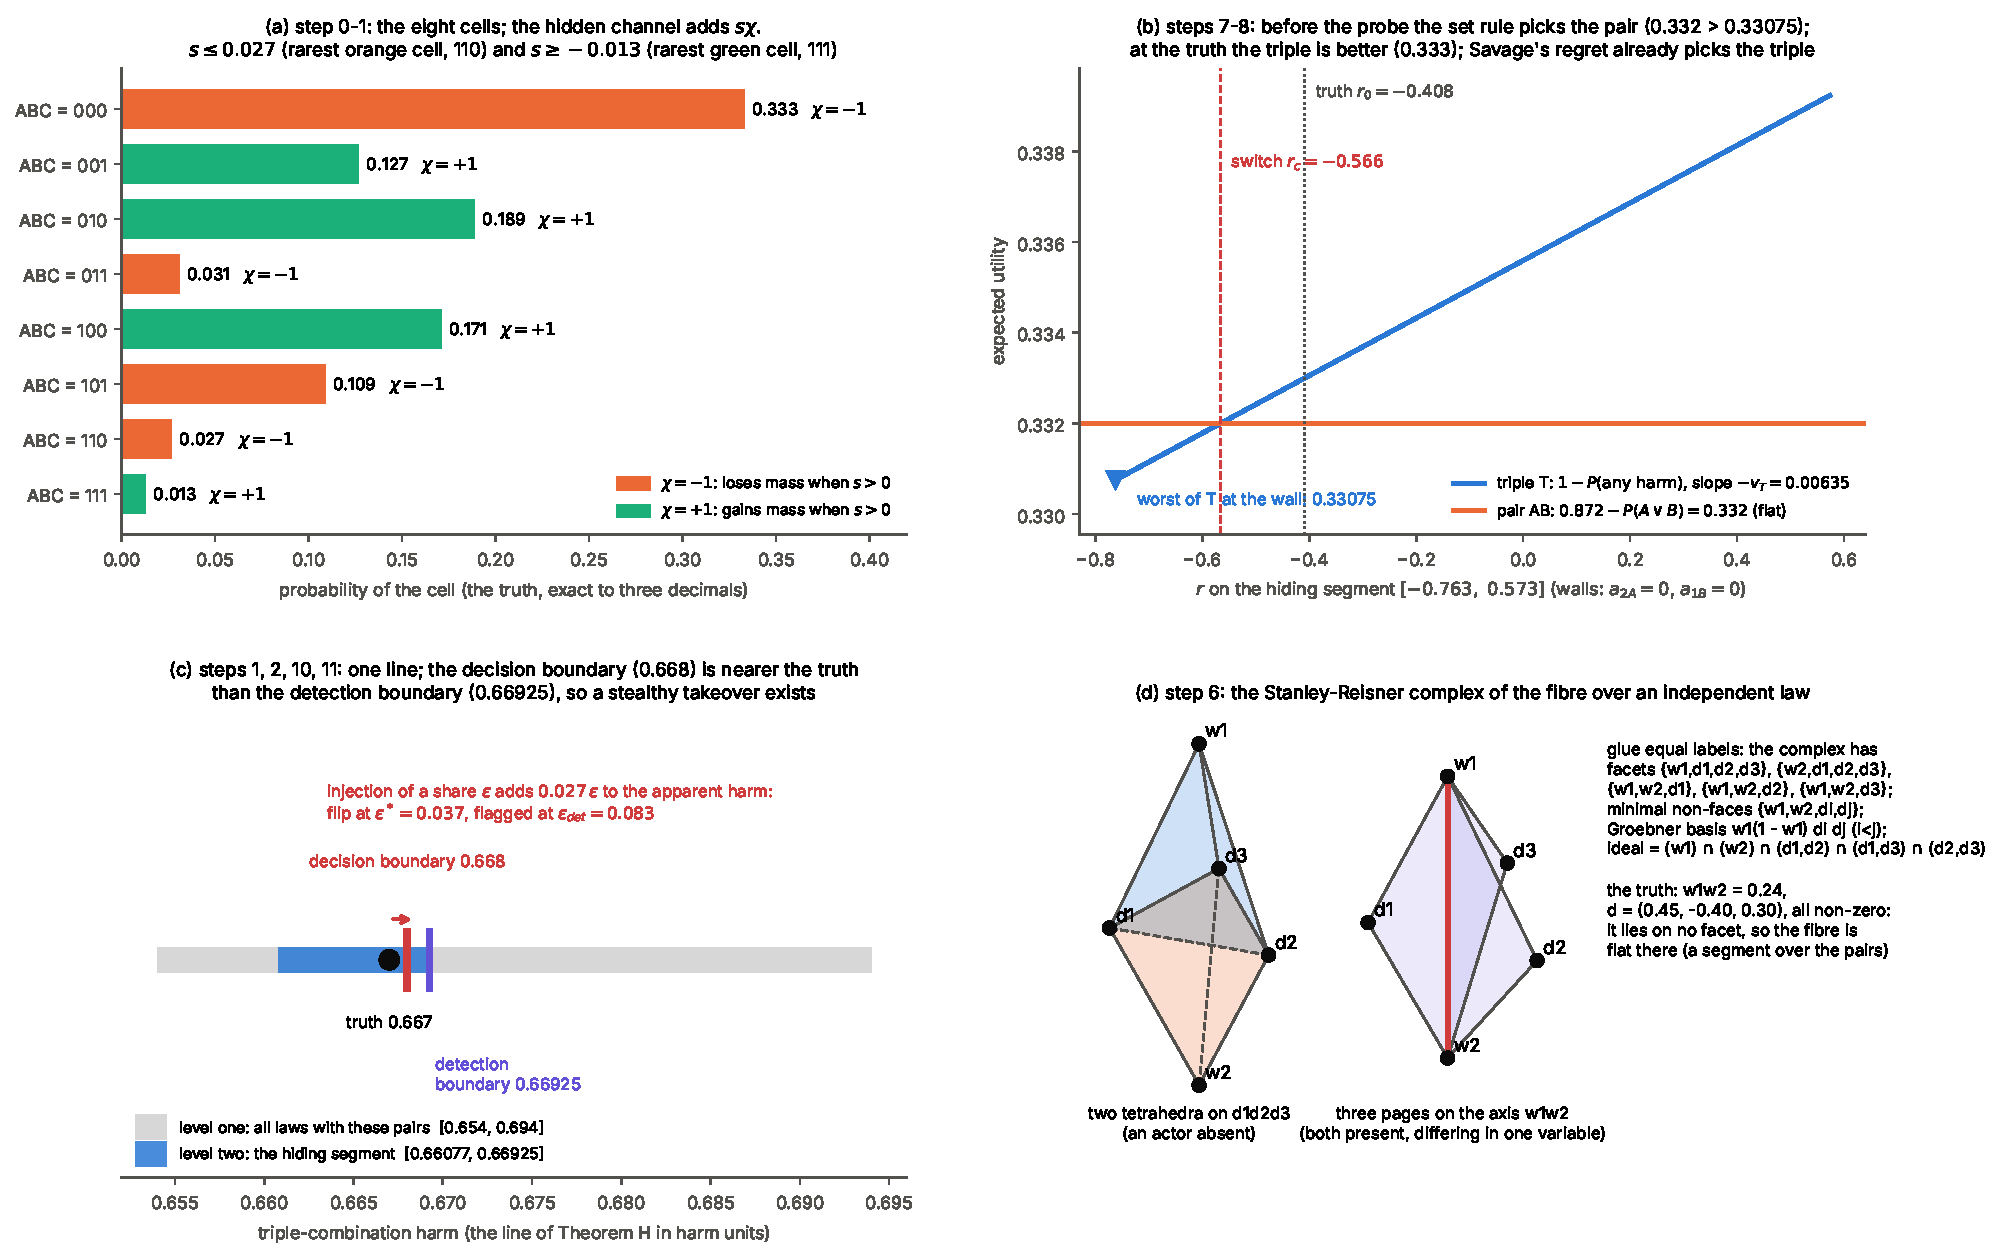
\includegraphics[width=\linewidth]{fig_worked.pdf}
\caption{The worked example. (a) The eight cells and the sign of the top Walsh character; the channel's capacity is set by the rarest
cell of each sign. (b) The decision on the hiding segment: before the probe the set rule picks the pair, while at the truth the triple is
better. (c) The line of \cref{thm:H} in harm units: level one (grey), level two (blue), the truth, the decision boundary and the
detection boundary. (d) The Stanley--Reisner complex of the fibre over an independent law, drawn as two tetrahedra and a three-page book
glued along equal labels.}\label{fig:worked}
\end{figure}

\begin{figure}[!htbp]\centering
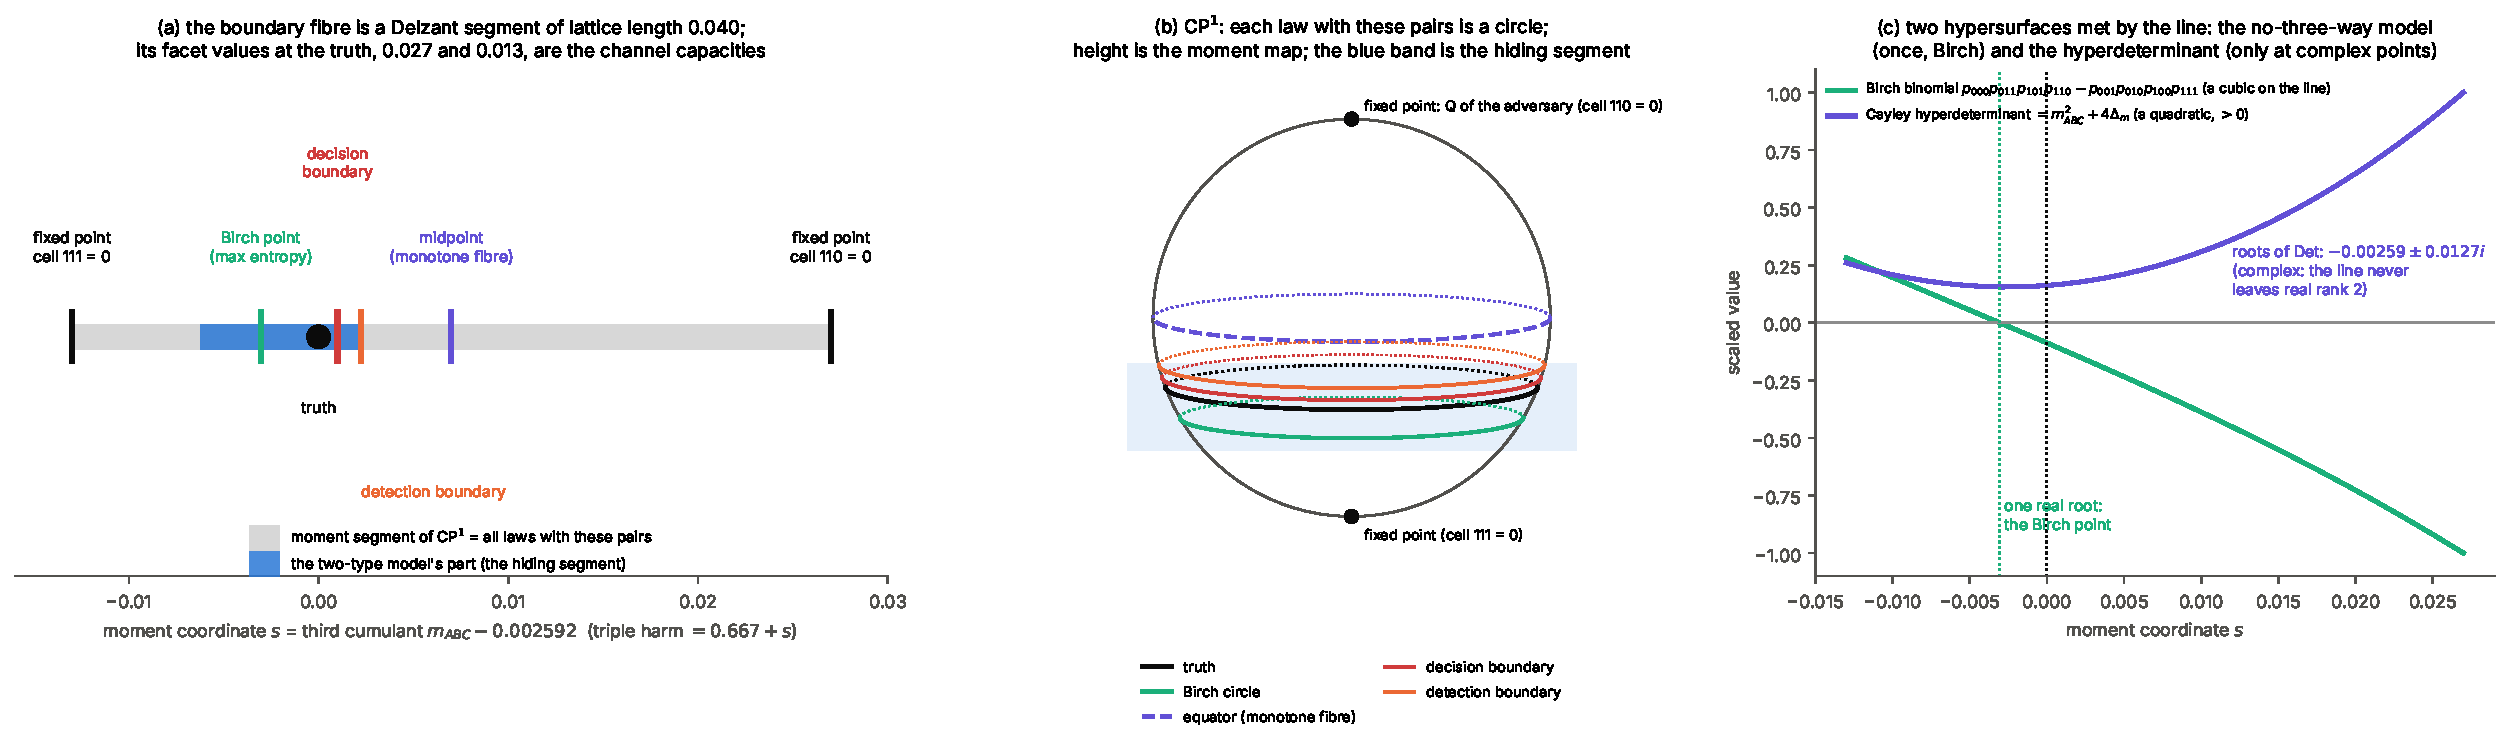
\includegraphics[width=\linewidth]{fig_toric.pdf}
\caption{Step~13, the toric reading of the worked example. (a) The moment segment of $\mathbb{CP}^1$ in the coordinate $s$ (the third
cumulant, shifted): its two fixed points, the truth, the Birch point, the monotone midpoint, the hiding segment and the two boundaries.
(b) The same data on the sphere: each law with these pair tables is a latitude circle. (c) The two hypersurfaces restricted to the line:
the no-three-way quartic becomes a cubic with one real root (the Birch point); Cayley's hyperdeterminant becomes $m_{ABC}^2+4\Delta_m$,
positive throughout.}\label{fig:toric}
\end{figure}

\paragraph{Step 14: the descent complex and the filtration, by hand.} Theorem~M (\cref{sec:descent}) says that the degrees and groups
of every obstruction come out of a construction. On the drug example the whole construction fits on a page
(\cref{fig:descent}).

\emph{The complex.} The contexts are $AB$, $BC$, $AC$, their overlaps $B$, $A$, $C$, and the empty context, whose single cell carries
the total mass. The nerve is a hollow triangle: three vertices and three edges, but no $2$-simplex, because $AB\cap BC\cap AC=\emptyset$.
The Čech complex of signed measures is
\[
C^0=\mathbb R^{4}\oplus\mathbb R^{4}\oplus\mathbb R^{4}\ \xrightarrow{\ d^0\ }\ C^1=\mathbb R^{2}\oplus\mathbb R^{2}\oplus\mathbb R^{2}\ \xrightarrow{\ d^1\ }\ C^2=\mathbb R,
\]
with dimensions $12$, $6$ and $1$. $d^0$ subtracts the two restrictions of a family to each overlap (\cref{fig:descent}(b)). It has
rank $5$, and $d^1$ has rank $1$. Hence
\[
H^0=12-5=7,\qquad H^1=(6-1)-5=0,\qquad H^2=1-1=0 .
\]
The $7$ compatible signed families are $3$ single rates, $3$ pair covariances and the total mass. The marginal map from the $8$ cells
of a signed law onto them has rank $7$. The one direction it loses is $\chi_{ABC}$, the line $s$ of Step~1. So the fibre of Step~1 is
exactly the kernel of descent, and nothing obstructs descent algebraically (check WD1--WD3).

\emph{The filtration, stage by stage.}
\begin{itemize}
\item \emph{D$_1$, gluing.} The pair tables come from one law, so $\lambda^*=1$. The liar-cycle inequality
  $P(A{=}B)+P(B{=}C)+P(A{\ne}C)\le2$ has value $1.40$ here. The liar cycle itself has $\lambda^*=0$ and value $3$.
\item \emph{D$_2$, signs.} The sign cochain on the graph $\Gamma$ of pairs has cycle product
  \[
  M_{01}M_{02}M_{12}=(-0.0432)(0.0324)(-0.0288)=4.03\times10^{-5}>0,
  \]
  so the class in $H^1(\Gamma;\mathbb Z/2)$ is $0$ and $\operatorname{sign}v=(+,-,+)$ solves it. The other solution, $(-,+,-)$, is the label
  switch: the kernel $H^0(\Gamma;\mathbb Z/2)=\mathbb Z/2$ (\cref{fig:descent}(c)). The ``exactly one harm'' law, uniform on $100$, $010$,
  $001$, has $M_{ij}=-1/9$ on every edge. Its cycle product is $-1/729<0$, so it has class $1$, and no two-type explanation exists
  although its tables glue.
\item \emph{D$_3$, moduli.} With three edges and three vertices the unsigned incidence matrix is invertible, so $\operatorname{coker}B=0$
  and the moduli are solved, not tested:
  \[
  |v_0|=\sqrt{\tfrac{M_{01}M_{02}}{M_{12}}}=0.2205,\qquad |v_1|=0.1960,\qquad |v_2|=0.1470,
  \]
  which is $\sqrt{0.24}\,(0.45,0.40,0.30)$. This is why three variables carry no model equation.
\item \emph{D$_4$, walls.} The walls cut $t\in[0.689,1.327]$, so the segment $R=[-0.763,0.573]$ is non-empty. A witness for this
  stage is a joint law ($\mu=(0.382,0.459,0.463)$) with both classes zero whose walls cross ($t_{lo}=1.095>t_{hi}=1.075$): signs and
  moduli solve, but no box of probabilities holds the types.
\item \emph{D$_5$, the triple.} $\hat r=r_0=-0.408$ lies inside $R$. The hidden channel moves $\hat r$ along the kernel of descent. Past
  $\varepsilon_{\det}=0.0833$ it leaves $R$; at $\varepsilon=0.10$, $\hat r=-0.834$, and the triple contradicts the pairs (check WD8).
\end{itemize}

\emph{Labels.} For one replicate of Study 13's design A1b ($n=1000$ per batch), the batches' triple moments form a $0$-cochain on a
simplex nerve (\cref{fig:descent}(d)). Its coboundary has energy $24\times(1.48\times10^{-5}+1.12\times10^{-4})$, split into
between-source and within-source parts. Source $C$'s statistic is $1.53$, under $c_s=2.39$: the adversary's four shifted batches,
$0.0052$ each, sit inside the band.

\begin{figure}[!htbp]\centering
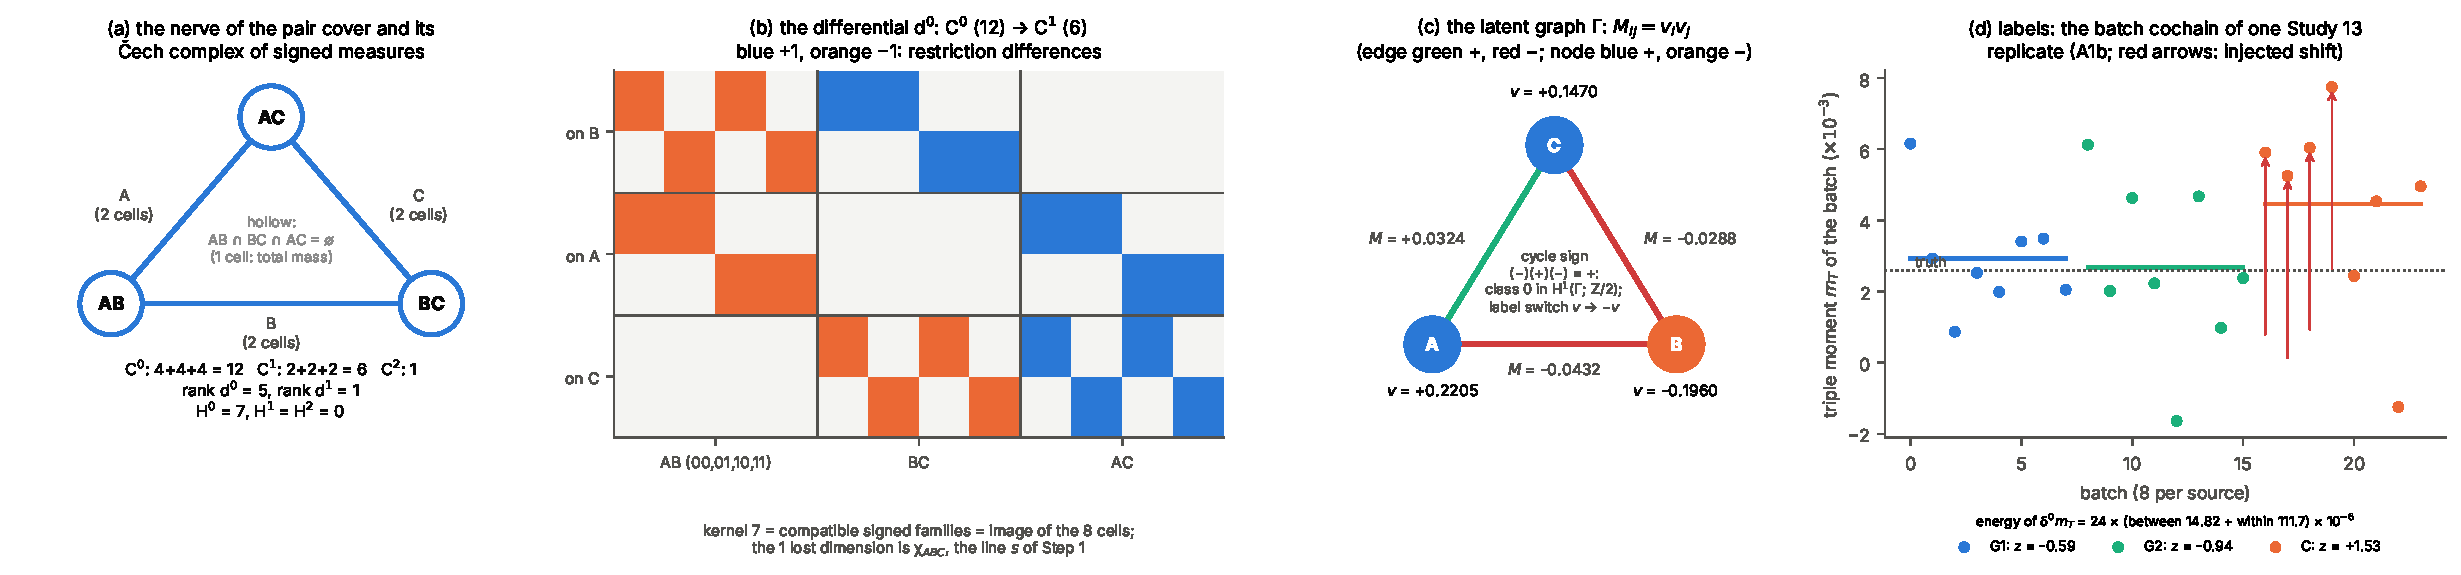
\includegraphics[width=\linewidth]{fig_descent.pdf}
\caption{The descent complex of the drug example. (a) The nerve of the pair cover, a hollow triangle, with the dimensions and ranks of
its Čech complex. (b) The differential $d^0$ as a matrix: each row compares the two restrictions to one overlap. (c) The latent graph
$\Gamma$: pair covariances on the edges and $v$ on the nodes. The cycle's sign is $+$, so $M=v_iv_j$ is solvable, uniquely up to the
label switch. (d) The labelled layer: the triple moments of the $24$ batches of one Study 13 replicate, with source means. The injected
shifts (arrows) stay under the source threshold.}\label{fig:descent}
\end{figure}

\section{The example with four variables, in stages}\label{sec:example4}
Add a fourth harm $D$ to the example of \cref{sec:example}, with probabilities $0.2$ and $0.7$ in the two types; everything else is
unchanged. The computation is staged so that each stage adds one layer of structure, and so that the three-variable interactions show
up one face at a time. The script \texttt{engine/worked\_example4.py} recomputes every number and asserts it (checks W4-1 to W4-14);
\cref{fig:worked4} draws the stages.

\paragraph{Stage 1: the law and its four faces.} The sixteen cells are exact four-decimal rationals, from $P(0000)=0.1809$ to
$P(1111)=0.0031$. Each triple of variables is a face: a $2\times2\times2$ table with its own line, capacities, Birch point and
hyperdeterminant, as in Step~13. The $ABC$ face is the three-variable example exactly. All four faces carry the same unseen coordinate,
$r_S=m_S/v_S=-0.408$ for every triple $S$, because there is one pair of types behind them. Each face's hyperdeterminant
$m_S^2+4\Delta_S$ is positive on its whole line.
\begin{center}\small
\begin{tabular}{lcccccc}\toprule
face & $m_S$ & $v_S$ & capacities & Birch point $s$ & three-way odds ratio & $r_S$\\\midrule
$ABC$ & $0.002592$ & $-0.006349$ & $0.027$, $0.013$ & $-0.00305$ & $0.569$ & $-0.408$\\
$ABD$ & $-0.00432$ & $0.010582$ & $0.027$, $0.013$ & $0.00233$ & $1.449$ & $-0.408$\\
$ACD$ & $0.00324$ & $-0.007936$ & $0.0486$, $0.0254$ & $-0.00557$ & $0.522$ & $-0.408$\\
$BCD$ & $-0.00288$ & $0.007055$ & $0.0252$, $0.0188$ & $0.00087$ & $1.132$ & $-0.408$\\\bottomrule
\end{tabular}
\end{center}

\paragraph{Stage 2: three-way interactions.} Along each face's line the log three-way odds ratio decreases strictly, and it is zero at
the face's Birch point. So a face's three-way interaction says on which side of its Birch point the truth lies: an odds ratio below
one means a larger triple moment than the Birch point's, as for $ABC$ and $ACD$ ($0.569$ and $0.522$), and above one a smaller, as for
$ABD$ and $BCD$ ($1.449$ and $1.132$). The two-type model ties the four
together through the single $r$, but they are not alike. The four-way odds ratio of the truth is $0.507$.

Now remove every interaction of order three or more at once. The global maximum-entropy law with the six pair tables, the pairwise
log-linear law found by iterative proportional fitting, is the four-variable Birch point. Its faces are \emph{not} their own Birch
points: marginalising it induces a small negative three-way interaction on every face, with odds ratios $0.977$, $0.985$, $0.960$ and
$0.965$. A law with no three-way interaction among four variables still shows three-way interaction among three of them. The
three-variable maximum-entropy answer of Step~13 and the four-variable one therefore differ: the $ABC$ triple moment is $-0.000456$
at the face's Birch point and $-0.000336$ under the global one.

\paragraph{Stage 3: the pair fibre is a smooth toric 5-fold.} All laws on $\{0,1\}^4$ with the six pair tables form a polytope $\Pi$
of dimension $16-1-4-6=5$. Its tangent lattice is the set of integer tables with zero one- and two-way margins. The four triple
characters and the four-way character span a sublattice of index $16$ in it, because sums such as $(\chi_{ABC}+\chi_{ABD})/2$ are
already integral; a saturated basis with entries $0,\pm1$ exists. In that lattice:
\begin{itemize}
\item $\Pi$ has $20$ vertices, found by exact enumeration, and $9$ facets. Only nine of the sixteen cells give facets, namely $0011$,
  $0110$, $0111$, $1001$, $1011$, $1100$, $1101$, $1110$ and $1111$; the other seven can never reach zero with these pair tables.
\item Every vertex lies on exactly five facets (simple), and at every vertex the five facet normals form a lattice basis (smooth). So
  $\Pi$ is Delzant, and its toric manifold $X_\Pi$ is a smooth compact toric 5-fold \cite{Delzant1988} with Euler characteristic $20$,
  the number of torus-fixed points.
\item The f-vector is $(20,50,54,31,9,1)$, and the h-vector is $(1,4,5,5,4,1)$. For a smooth projective toric variety the h-vector of
  the simple polytope gives the even Betti numbers, so the Poincaré polynomial of $X_\Pi$ is $1+4t^2+5t^4+5t^6+4t^8+t^{10}$. It is
  palindromic (Poincaré duality), and $b_2=4$ is the number of facets minus the dimension.
\item At the truth the facet values are the probabilities of the nine facet cells, so these nine numbers are the Kähler data,
  $[\omega]=\sum_c P(c)\,[D_c]$ \cite[Prop.~2.2]{Coupling}. The lattice volume of $\Pi$, which is the symplectic volume of $X_\Pi$, is
  $1.27\times10^{-8}$.
\item Projecting $\Pi$ to two faces' triple moments is the moment map of a two-dimensional subtorus. For five of the six pairs of
  faces the image is the product of the two faces' lines, a rectangle: those two three-way structures can be chosen independently. For
  $ACD$ and $BCD$, which share the pair $CD$, the image is a pentagon, a rectangle with one corner cut by $0.002$. When both channels
  are pushed to their extremes at once they compete for the same rare cells, and the two faces' three-way moments are coupled. This is
  the corner-cutting of the coupling paper's $2\times3$ family, here appearing inside a projection.
\end{itemize}
The toric picture does not always survive. Moving the fourth harm (Stage~6) shows smooth chambers ($a_{2D}=0.5$ and $0.7$), a wall
where $\Pi$ is not simple ($a_{2D}=0.6$: $17$ vertices, some on six facets), and, at $a_{1D}=0.3$, a chamber where $\Pi$ is simple but
some vertices have index $2$: the moment polytope of a toric orbifold \cite{LermanTolman1997}, not of a manifold. In $50$ random laws and
random two-type truths the fibre was always simple and never smooth (check W4-14). This answers, for the four-variable pair fibre, the question of \cite[Prop.~10.5]{Coupling}
of where the toric picture stops: it depends on the chamber.

\paragraph{Stage 4: the model is a conic arc.} Inside the five coordinates (four triple moments and the four-way moment) the two-type
laws with these pair tables satisfy three linear equations, $m_S/v_S=m_{S'}/v_{S'}$, and one quadric, $m_{ABCD}=v_{ABCD}(r^2+1)$ with
$v_{ABCD}=0.001555$. So the hiding segment is an arc of a plane conic in the 5-dimensional polytope; on any two faces it projects to a
straight segment through the origin. The fourth harm's own box walls allow $t\in[0.408,1.633]$, which contains the three-variable
range $[0.689,1.327]$. So here the walls are slack, the segment is the same $r\in[-0.763,0.573]$, and the $ABC$ harm interval stays
$[0.66077,0.66925]$. A more extreme fourth harm would cut it.

\paragraph{Stage 5: the decision and the hidden channel with four variables.} The decision of Step~7 is unchanged: the pair before
the probe, the triple at the truth. Three numbers change.
\begin{itemize}
\item \emph{The channel is narrower.} The $ABC$ channel is now $P+s\chi_{ABC}$ on sixteen cells, and its capacity is the rarest
  sixteen-cell probability with the needed sign, $0.0099$ (cells $1101$ and $1110$). It moves the face by $2s$ (\cref{thm:F}(4)), so
  the capacity in face units is $0.0198$, against $0.027$ with three variables. The flip needs $\varepsilon^*=0.001/0.0198=5.05\%$
  (against $3.7\%$), and the triple contradicts the pairs at $0.00225/0.0198=11.4\%$. The whole fibre still allows $m_{ABC}$ anywhere
  in the three-variable line $[-0.0104,0.0296]$, but only by moving other faces too.
\item \emph{A second triple catches it.} The channel moves $\hat r_{ABC}$ and leaves the other three at $-0.408$
  (\cref{cor:secondtriple}). With $10^5$ records per window, the standard deviation of $\hat r_{ABC}-\hat r_{ABD}$ is $0.047$, so a
  two-sided test at level $0.05$ fires once $3.12\,\varepsilon>1.96\cdot0.047$, at $\varepsilon=3.0\%$, before the flip at $5.05\%$.
\item \emph{Staying on the model is expensive.} An adversary who keeps every pair table and every model equation must make the observed
  law the two-type law at some $r$. The least share that reaches the switch point is exactly $1-\min_x P_{r_c}(x)/P(x)=18.3\%$; the walls
  follow at $42.2\%$. With three variables the same formula gives $3.7\%$, the hidden channel itself.
\end{itemize}
So the fourth variable does not change what is hidden, but it changes what hiding costs: from $3.7\%$ and invisible to $5.05\%$ and
caught at $3.0\%$, or $18.3\%$ to stay invisible.

\paragraph{Stage 6: chambers.} The table of Stage~3's last paragraph: $a_{2D}=0.5$ and $0.7$ give smooth fibres with $20$ vertices and
$9$ facets; $a_{2D}=0.6$ lies on a wall, with $17$ vertices and some vertices on six facets; $(a_{1D},a_{2D})=(0.3,0.7)$ gives $28$
vertices, $10$ facets and vertex index $2$.

\begin{figure}[!htbp]\centering
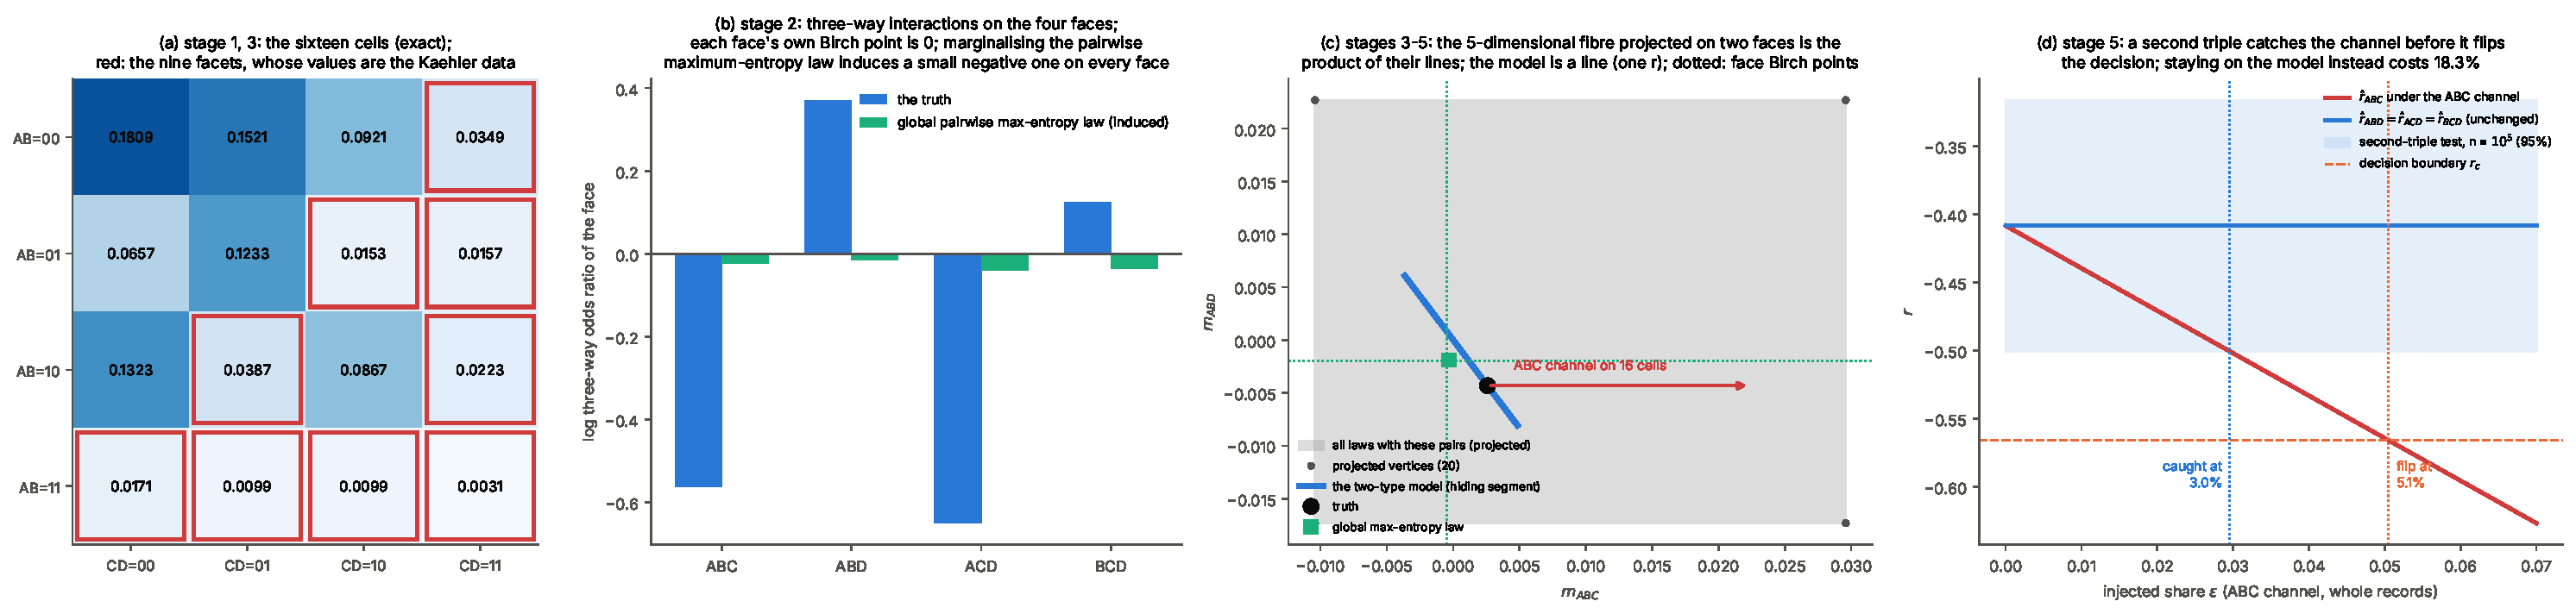
\includegraphics[width=\linewidth]{fig_worked4.pdf}
\caption{The example with four variables. (a) The sixteen cells; red outlines mark the nine facets of the pair fibre, whose
probabilities are the Kähler data. (b) Three-way interactions on the four faces: the truth's, and those induced on the faces by the
global pairwise maximum-entropy law. (c) The 5-dimensional fibre projected on the $ABC$ and $ABD$ triple moments (a rectangle, the
product of the two faces' lines), the two-type model, the truth, the global maximum-entropy law, and the $ABC$ channel. (d) Under the
$ABC$ channel only $\hat r_{ABC}$ moves; a second-triple test with $10^5$ records per window fires at $3.0\%$, before the flip at
$5.05\%$.}\label{fig:worked4}
\end{figure}

\paragraph{Stage 7: the filtration with four variables.} Two stages that are empty at $m=3$ become tests at $m=4$ (\cref{fig:filtration}).
\begin{itemize}
\item \emph{D$_3$.} $\operatorname{coker}B$ now has dimension $2$, spanned by the two log tetrad ratios $\log(M_{01}M_{23}/M_{02}M_{13})$ and
  $\log(M_{02}M_{13}/M_{03}M_{12})$. Both are $0$ on the truth. Injecting a product law at $\varepsilon=0.1$ (\cref{thm:E}(4)) keeps every
  cycle sign but moves them to $-1.65$ and $-0.49$.
\item \emph{D$_5$.} The four triple windows give a $0$-cochain $r_S$, and the model requires $\delta r=0$. On the truth all four equal
  $0.408$. This is $r_0$ of Step~2 up to sign: the types are relabelled so that $v_A>0$, which is the label switch of D$_2$ in action.
  Half-capacity $\chi_{ABC}$ injection at $\varepsilon=0.05$ moves $r_{ABC}$ to $0.486$ and leaves the other three at $0.408$. The
  obstruction moves up exactly one level (check WD10).
\end{itemize}
Every stage now has a witness that passes the earlier stages and fails there. Each stage also computes a value that the earlier ones did
not:
\begin{itemize}
\item the gluable fraction;
\item the cycle sign;
\item the solved moduli, or the tetrads;
\item the segment;
\item the coherence of $r_S$;
\item the between-source energy.
\end{itemize}

\begin{figure}[!htbp]\centering
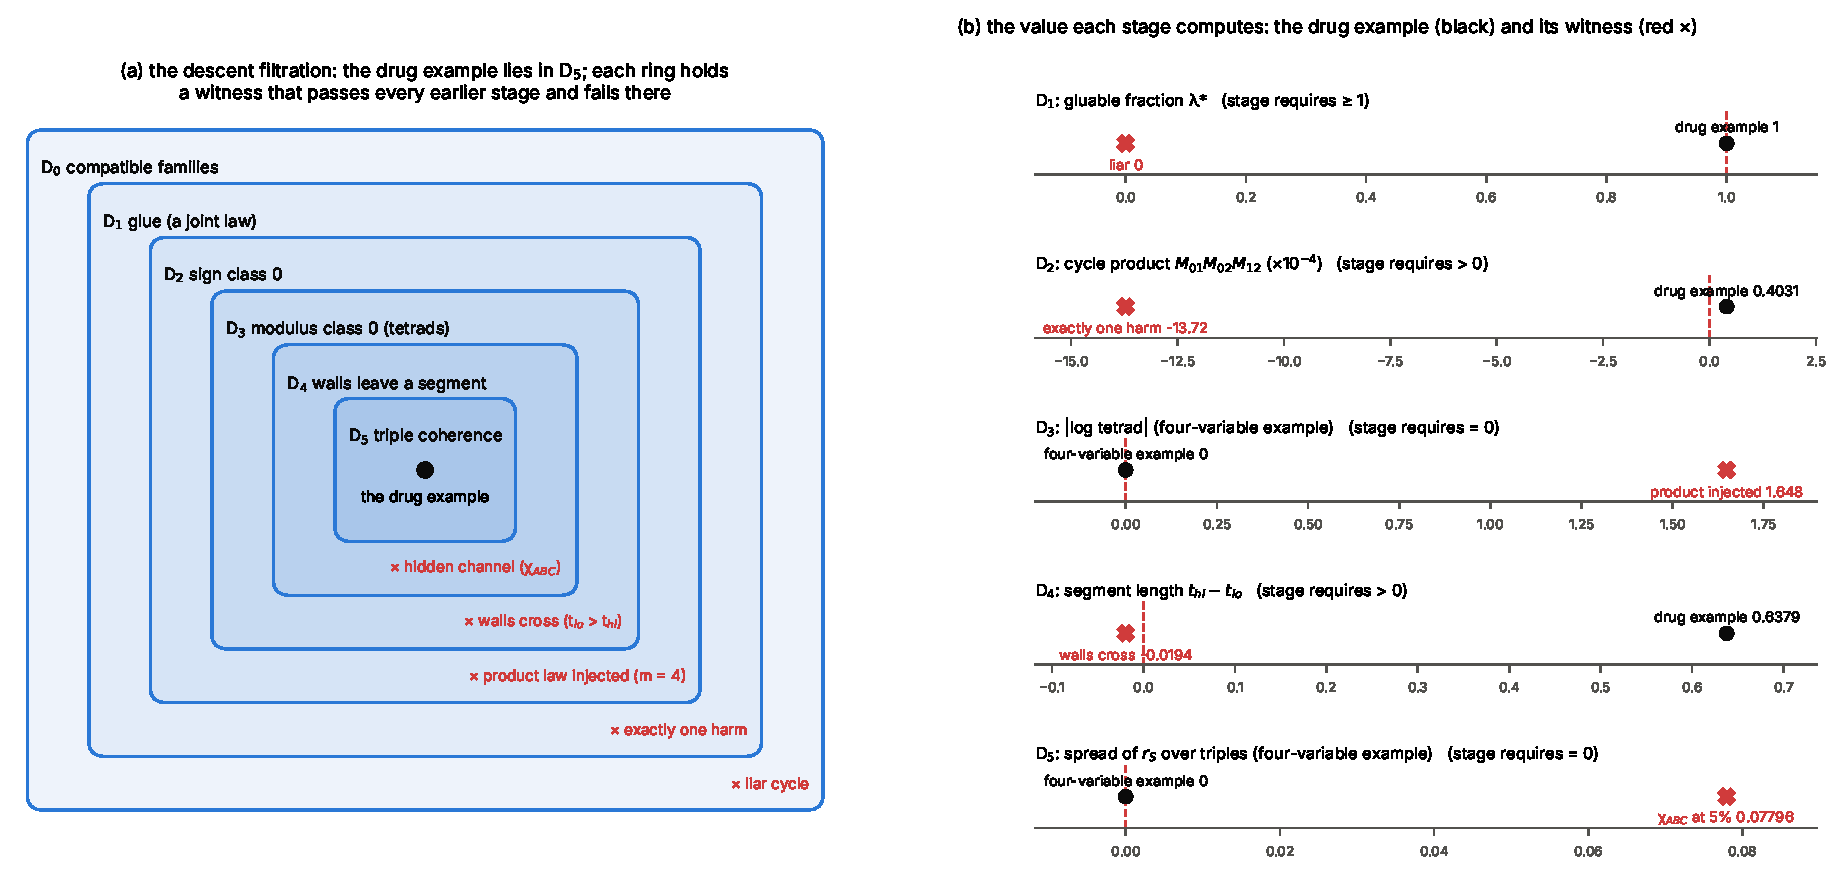
\includegraphics[width=\linewidth]{fig_filtration.pdf}
\caption{The descent filtration on the worked examples. (a) The nested stages $D_0\supset\dots\supset D_5$. The drug example lies in
$D_5$, and each ring holds a witness that passes every earlier stage and fails there. (b) The value each stage computes, for the
example (black) and its witness (red): $\lambda^*$; the cycle product; the log tetrads (four variables); the segment length; the
spread of $r_S$ over the triples (four variables). The dashed line is the stage's requirement.}\label{fig:filtration}
\end{figure}

\section{Part II, continued. Sources: a trusted source that is sometimes adversarial}\label{sec:sources}
Theorems E--H let the adversary inject into the whole pool, and the regulator sees only the pooled tables. In practice data arrive from
\emph{sources}, in \emph{batches}, and the decision maker knows where each table came from and nothing else about provenance. The
dangerous case is not a hostile source, which can be dropped once it is identified. It is a \emph{trusted} source that is genuine most
of the time and adversarial in some batches, and that adds just enough to tilt the decision or to delay it. Writing such a source off
throws away its genuine data. Trusting it lets the adversary in. This section shows what the labels buy, using the worked example of
\cref{sec:example} as the truth.

\paragraph{Sources, batches and sections.} There are three sources, $G_1$, $G_2$ and $C$, each sending $K_C$ batches. A batch is the
triple window (the probe) with $n$ records and the three pair windows with $\rho n$ records each, since pair tables come from large
registries. Every table is a \emph{section} over its context, labelled by (source, batch). All sections come from one population, so
they must glue. Source $C$ is genuine in most batches. In some of them a share $\varepsilon_b$ of the records is drawn from the hidden
channel $Q=P+s\chi_T$ of \cref{thm:F}. That leaves every single and pair table unchanged and moves the triple moment by exactly
\[
m_T\bigl((1-\varepsilon_b)P+\varepsilon_bQ\bigr)=m_T(P)+\varepsilon_b s,
\]
because the coefficient of $\chi_T$ in the centred triple moment is $\prod_i\sum_{x_i}(2x_i-1)(x_i-\mu_i)=1$. The pair sections therefore
always glue, and the triple sections can fail to glue only along one coordinate, $m_T$. The gluing test is a test on that coordinate.

\paragraph{Monad and comonad.} The provenance comonad of \cref{sec:inj} now has observable labels: $W=L\times(-)$ with
$L=\{\text{sources}\}\times\{\text{batches}\}$. The family of batch laws is an element $\Pi=\frac1K\sum_b\delta_{P_b}$ of $D(DX)$,
where $D$ is the distribution monad. \emph{Pooling is the monad's multiplication} $\mu:D(DX)\to DX$, which averages the batch laws. The
data come from one population exactly when $\Pi$ lies in the image of the unit $\eta:DX\to D(DX)$, that is, when all batch laws are
equal: this is the gluing condition. Injection in some batches moves $\Pi$ off the image of $\eta$. Since $\mu\circ\eta=\mathrm{id}$,
pooling cannot tell $\Pi$ from $\eta(\mu\Pi)$: the adversary's footprint lies in the fibre of $\mu$. A rule that pools factors through
the counit of $W$, which forgets the labels. A rule that tests gluing is a coKleisli arrow $WX\to A$ that does not factor through the
counit. The comonad supplies the labels that make the monad's inner layer visible. As in \cref{sec:inj}, this framing names the
situation; the results come from the following statistics.

\paragraph{The gluing filter.} Write $\hat m_b$ for batch $b$'s triple moment, $\sigma_m^2$ for the variance of its influence function
(per record), and $\sigma_b=\sigma_m/\sqrt n$. The filter tests two covers, the fine one first.
\begin{enumerate}
\item \emph{Batches.} $z_b=(\hat m_b-\tilde m)/(\sigma_b\sqrt{1+1/K_C})$, where $\tilde m$ is the median of the three source means.
  Triple sections with $|z_b|>c_b$ are dropped.
\item \emph{Sources.} For each source $j$, $Z_j$ compares its pooled triple moment (kept batches) with that of the other two. If the
  largest $|Z_j|$ exceeds $c_s$, that source's remaining triple sections are dropped.
\end{enumerate}
Pair sections are always kept, and the decision is taken on the colimit of the sections that remain. The median reference matters.
With one compromised source, the median lies between the two genuine source means, so a strongly shifted source cannot pull genuine
batches out of the pool. A leave-one-out reference can: it drops genuine batches on the far side (swamping), and that biases the pool
toward the adversary. The Gaussian model showed this before the filter was fixed.

\setcounter{theorem}{9}% Theorem J (I is skipped to avoid confusion with Part I)
\begin{theorem}[sources and bands]\label{thm:J}
Let source $C$ hold a share $\pi$ of the triple records, and let the other sources be genuine.
\begin{enumerate}
\item[(1)] \emph{Pooling.} A rule that pools faces a whole-pool injection of share $\pi\bar\varepsilon_C$, where $\bar\varepsilon_C$ is
  $C$'s average share. All of \cref{thm:F}'s budgets apply, divided by $\pi$. For two triple sections with shares $\varepsilon$ and
  $\varepsilon'$, the gluable fraction is $\lambda^*=1-|\varepsilon-\varepsilon'|\,\mathrm{TV}(P,Q)$. Hence $1-\lambda^*$ is a lower
  bound on the difference in contamination (Tier 1).
\item[(2)] \emph{The band.} If $C$'s source statistic has mean $a$, then $C$ moves the pooled triple moment by exactly
  \[
  a\sqrt{\pi/(1-\pi)}\quad\text{pooled standard errors},
  \]
  whatever $K_C$, $K$ and $n$ are. An adversary that keeps its exposure risk at most $\beta$ has $a\le c_s-\Phi^{-1}(1-\beta)$. It therefore
  moves the pooled estimate by at most
  \[
  B=\bigl(c_s-\Phi^{-1}(1-\beta)\bigr)\sqrt{\pi/(1-\pi)}
  \]
  standard errors, \emph{at every sample size}. Its per-batch share shrinks like $1/\sqrt n$: the adversary rides inside the noise band.
\item[(3)] \emph{No tilt.} Let $d$ be the settling radius (\cref{thm:D}) and $\kappa=\sigma_m/(|v_T|\tau)\le1$. Under the filter, such
  an adversary settles the decision on the wrong act with probability at most
  $\Phi\bigl(\kappa B-z-d\sqrt N/\tau\bigr)\le\Phi(B-z)$, up to the genuine rate. This tends to $0$ as $N$ grows. Under pooling, a fixed
  share of $C$ with $\pi\bar\varepsilon_C\in(\varepsilon^*,\varepsilon_{\det})$ settles on the wrong act with probability tending to
  one.
\item[(4)] \emph{Delay.} The sample size at which the decision settles half the time moves from $(z\tau/d)^2$ to at most
  \[
  N_{1/2}\le\bigl((z\tau+B\sigma_m/|v_T|)/d\bigr)^2\approx\bigl((z+B)/z\bigr)^2(z\tau/d)^2 .
  \]
\item[(5)] \emph{Localisation.} A gluing failure can be localised down to the finest cover whose sections are less noisy than the
  shift. A shift $\Delta$ in one batch is seen at the batch level once $\Delta\gtrsim c_b\sigma_b$. The same total shift spread over $k$
  batches is invisible there when $\Delta/k<c_b\sigma_b$, and only the source level sees it. With two sources a failure cannot be
  localised, since $Z_1$ and $Z_2$ are opposite in sign and proportional in size. With three, the median makes the batch test immune to
  swamping by a single compromised source.
\end{enumerate}
\end{theorem}

\begin{proof}
(1) $\mu$ is linear, so the pooled law is $(1-\pi\bar\varepsilon_C)P+\pi\bar\varepsilon_CQ$. For two laws on one context,
$\lambda^*=\sum_x\min(P_\varepsilon(x),P_{\varepsilon'}(x))=1-\mathrm{TV}(P_\varepsilon,P_{\varepsilon'})$, and
$P_\varepsilon-P_{\varepsilon'}=(\varepsilon-\varepsilon')(Q-P)$.
(2) Let $D$ be $C$'s mean shift. Its statistic has mean
$a=D/\bigl(\sigma_m\sqrt{1/(\pi N)+1/((1-\pi)N)}\bigr)$. The pooled shift is $\pi D$, and the pooled standard error is
$\sigma_m/\sqrt N$, so the ratio is $a\,\pi\sqrt{1/\pi+1/(1-\pi)}=a\sqrt{\pi/(1-\pi)}$. The exposure probability is
$\Phi(a-c_s)+\Phi(-a-c_s)\ge\Phi(a-c_s)$.
(3) The triple part of the decision statistic $\hat r-\hat r_c$ is $(\hat m_T-m_T)/v_T$, so the variance of its triple part is
$\sigma_m^2/v_T^2$ (check SR5). Settling on the wrong act needs the shift to exceed $d+z\tau/\sqrt N$. When the filter keeps $C$, the
statistic is conditioned on $|Z_C|\le c_s$, which only lowers the shift, because the pooled estimate and $Z_C$ are positively
correlated. When the filter drops $C$, the pool is genuine. Under pooling with a fixed share, the shift $\pi\bar\varepsilon_Cs/|v_T|$
exceeds $d$ by a fixed amount while the noise shrinks.
(4) The median of the settling statistic crosses $z\tau/\sqrt N$ when $d-B\sigma_m/(|v_T|\sqrt N)=z\tau/\sqrt N$. Exposure only helps
the decision maker.
(5) The batch statistic of a single shifted batch has mean $\Delta/\sigma_b$ up to the factor $\sqrt{1+1/K_C}$. With two sources,
$\hat m_1-\hat m_{12}$ and $\hat m_2-\hat m_{12}$ are proportional with opposite signs. The median of three numbers, one of them
arbitrary, lies between the other two.
\end{proof}

The theorem turns the adversary's ``just enough'' into geometry. Gluing is tested on a single coordinate, the fibre coordinate $m_T$ of
\cref{thm:H}. The adversary's operating region is a band of fixed width, $B$ standard errors, around the genuine estimate. Because the
standard error shrinks, the band narrows with $N$ and eventually clears the switch. So the filter turns every undetected tilt into a
delay, and the delay is bounded. With $c_s=2.394$ (Bonferroni over three sources) and $\pi=1/3$: $B=1.69$ at exposure risk one half,
and $B=1.10$ at exposure risk $0.2$. Both are below $z=1.96$, so an adversary that stays hidden cannot even make a wrong settlement
likely. The delay factor is at most $((z+B)/z)^2=3.5$ and $2.4$. The adversary pays a vanishing share for it: on the worked example's
truth, $4.4\%$ of the records in half of $C$'s batches at $N=192{,}000$ (\cref{tab:study13design}).

\paragraph{Tier 2.} If every source were compromised alike ($\pi\to1$), the band $B$ would be unbounded. No gluing test sees a shift
common to all sections, $\lambda^*=1$, and only the geometry is left: the walls (\cref{thm:F}(3)), the model's equations at $m\ge4$
(\cref{thm:G,thm:H}) and a second triple. The labels help exactly as far as the sources disagree.

\section{Study 13: a trusted source that is sometimes adversarial}\label{sec:study13}
Study 13 was registered and frozen before any registered design was simulated
(\texttt{engine/\allowbreak study13\_sources/\allowbreak PREREG\_study13.md}). The checks SR1--SR10 and the smoke runs used random
truths and an invented truth; on the registered truth only the Gaussian model was used. Before freezing, the filter's order was changed
on the strength of that model, and the change is disclosed in the registration (swamping, above).

\paragraph{Design.} The truth and the decision are those of \cref{sec:example}: approve the triple ($T$) or the pair ($P$), with the
switch at triple harm $0.668$ against a truth of $0.667$. There are three sources with $K_C=8$ batches each, triple windows of $n$
records, and pair windows of $25n$. The hidden channel uses $s=0.027$. The thresholds are $c_b=3.078$ and $c_s=2.394$, Bonferroni at
family-wise $0.05$, and $z=1.96$. The adversary knows $P$, $n$, $K$ and the thresholds, but not the noise. Five adversaries are
compared (\cref{tab:study13design}):
\begin{itemize}
\item none (A0);
\item \emph{sometimes, just enough}: $4$ of $C$'s $8$ batches, at exposure risk $0.2$ (A1) or $0.5$ (A1b);
\item \emph{concentrated}: A1's source shift in one batch (A3);
\item \emph{tuned to pooling}: a share of $0.18$ in every batch of $C$ (A2), so a pooled share of $0.06$, in the middle of the stealth
  window $(\varepsilon^*,\varepsilon_{\det})=(0.037,0.083)$.
\end{itemize}
Four rules see the same data:
\begin{itemize}
\item naive pooling;
\item the gluing filter;
\item an oracle that knows $C$ and drops its triple sections;
\item writing $C$ off entirely.
\end{itemize}
There are $N=24n$ triple records in all, from $12{,}000$ to $192{,}000$, with $2000$ replicates per cell.

\begin{table}[!htbp]\centering\small
\begin{tabular}{rrcccc}\toprule
$n$ per batch & $N$ & A1 (4 batches) & A1b (4 batches) & A3 (1 batch) & A2 (8 batches)\\\midrule
500 & 12{,}000 & 0.177 & 0.274 & 0.710 & 0.18\\
1000 & 24{,}000 & 0.125 & 0.193 & 0.502 & 0.18\\
2000 & 48{,}000 & 0.089 & 0.137 & 0.355 & 0.18\\
4000 & 96{,}000 & 0.063 & 0.097 & 0.251 & 0.18\\
8000 & 192{,}000 & 0.044 & 0.068 & 0.177 & 0.18\\\bottomrule
\end{tabular}
\caption{Study 13: the injected share in each adversarial batch of source $C$. ``Just enough'' shrinks like $1/\sqrt n$; the fixed
share does not.}\label{tab:study13design}
\end{table}

\begin{table}[!htbp]\centering\small
\begin{tabular}{p{0.06\linewidth}p{0.55\linewidth}p{0.31\linewidth}}\toprule
& prediction & outcome\\\midrule
H1 & right-rate within $0.05$ of the Gaussian model in $\ge90\%$ of the 100 cells, within $0.08$ in all & holds: 100 of 100; largest gap $0.031$\\
H2 & filter's wrong-rate $\le0.05$ everywhere; pooling under A2 wrong $\ge0.75$ at $192$k; filter within $0.05$ of the oracle under A2 for $N\ge48$k & holds: $\le0.020$; $0.877$; gap $\le0.006$\\
H3 & half-way points within $15\%$ of prediction for A0, A1, A1b; oracle $\ge$ filter under A1b for $N\ge24$k & holds: $24.7$k, $52.8$k, $55.7$k against $24.6$k, $53.0$k, $56.6$k; yes\\
H4 & A3's batch removed $\ge0.90$, $C$ dropped $\le0.10$, filter within $0.05$ of A0; under A0 a source dropped $\le0.08$ and filter within $0.04$ of pooling & holds: $0.96$--$0.97$; $0.011$--$0.017$; $\le0.025$; $\le0.044$; $\le0.012$\\
H5 & at $192$k the worst right-rate over adversaries is $\ge0.85$ for the filter and $\le0.05$ for pooling & holds: $0.918$ and $0$\\\bottomrule
\end{tabular}
\caption{Study 13: registered predictions and outcomes (2000 replicates per cell).}\label{tab:study13}
\end{table}

All five predictions held (\cref{tab:study13,fig:sources}). Without labels the adversary takes the decision over. Under pooling, a
share of $0.18$ in source $C$'s batches settles the wrong act in $88\%$ of replicates at $N=192{,}000$, and nothing is flagged. With
labels, the same attack is caught by its own growth: $C$'s gluing statistic grows like $\sqrt N$ (\cref{fig:sources}(c)), and the filter
matches the oracle that knows $C$ to within $0.006$. The adversary that stays hidden only delays. Its statistic rides flat under $c_s$,
and the filter's half-way point moves from $24.7$k to $52.8$k records (A1) and $55.7$k (A1b), as Theorem~\ref{thm:J}(4) bounds
($59$k and $85$k for an adversary that is never exposed; exposure, which drops $C$'s triples, is what keeps A1b close to A1). At no sample size does the filter settle on the wrong act in more than $2\%$ of replicates. A
concentrated attack is localised: the poisoned batch is removed $97\%$ of the time, $C$'s seven genuine batches stay in, and the filter
then beats both the oracle and writing $C$ off, because it keeps $C$'s genuine triples. On genuine data the filter costs at most
$0.012$ in right-rate.

The price of not knowing which source is compromised is the gap between the filter and the oracle under the tuned adversary, about
$0.16$ in right-rate at $48$k. No test on these tables can close it. The adversary sits inside the noise band by construction, and only
information beyond the tables (an audit of $C$, a second triple) can. Note also where pooling looks good: under A1 at $192$k pooling
($0.976$) beats the filter ($0.950$), because the tuned shift is small at that size and the filter sometimes drops $C$'s genuine data.
That is why the comparison that matters is the worst case over adversaries (H5), not any single attack.

\begin{figure}[!htbp]\centering
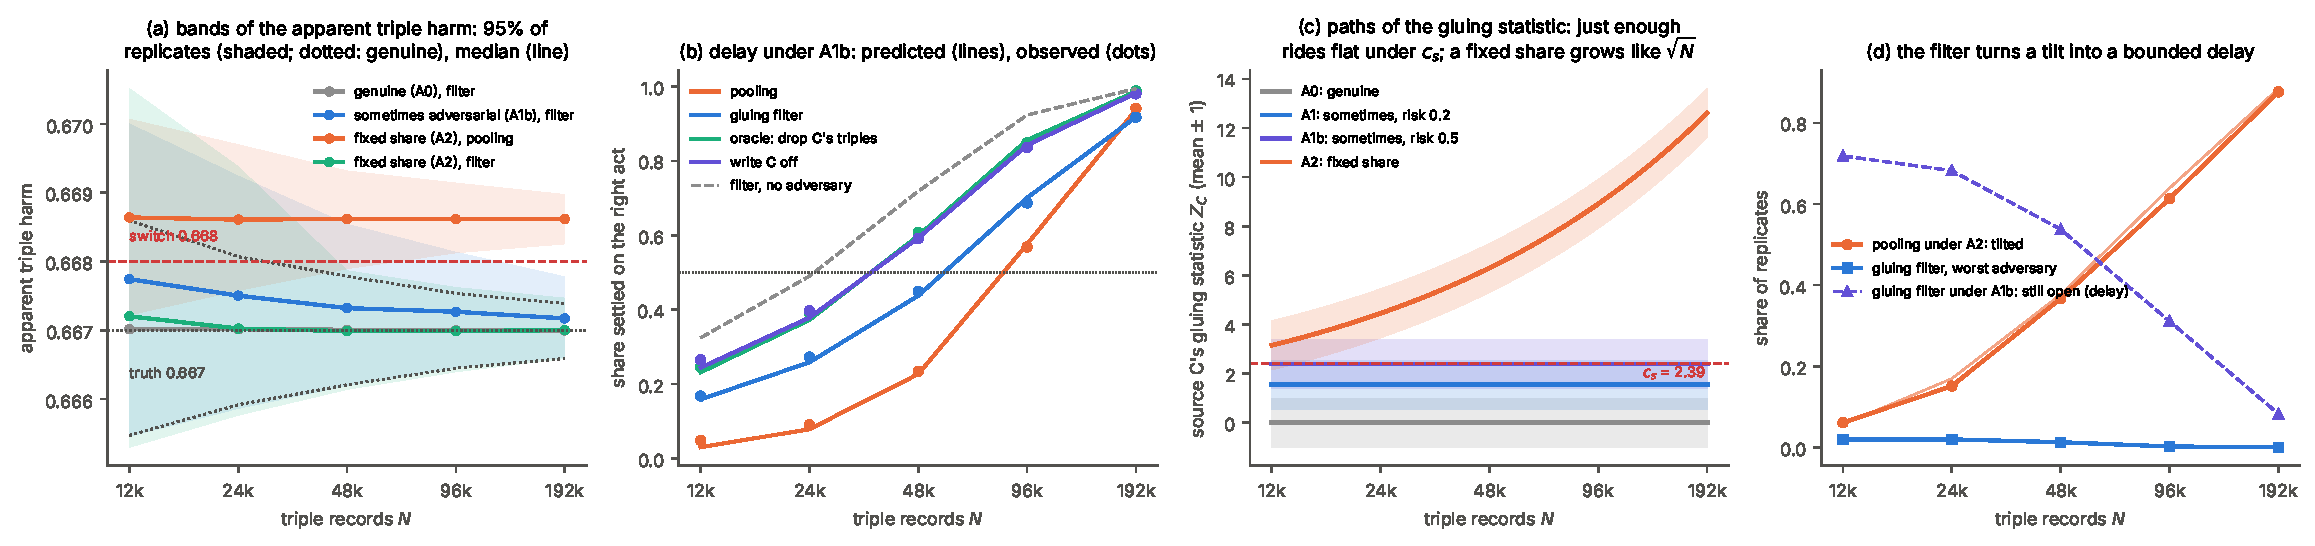
\includegraphics[width=\linewidth]{fig_sources.pdf}
\caption{Study 13. (a) Overlaid bands of the apparent triple harm (95\% of replicates). Pooling under a fixed share sits above the
switch and never comes back. The filter under the sometimes-adversarial source is shifted toward the switch by a band of fixed width in
standard errors, which shrinks and clears the switch. (b) Settling curves under A1b: the adversary delays the filter (blue) but cannot
stop it. The oracle (green) and writing $C$ off (violet) settle earlier, and pooling (orange) later. (c) Paths of $C$'s gluing statistic
(Gaussian model, mean $\pm1$): just-enough adversaries stay flat under $c_s$ at every $N$, while a fixed share grows like $\sqrt N$. (d)
Pooling is tilted with probability rising to $0.88$; the filter's wrong-rate under its worst adversary stays below $0.02$, and what is
left is the delay (open decisions under A1b).}\label{fig:sources}
\end{figure}

\paragraph{Tearing.} The filter's decision is a discontinuous function of the data. When $|Z_C|$ crosses $c_s$, $C$'s triple sections
leave the pool and the estimate jumps by $\pi D$. This is a tear in the decision map, along the hypersurface $|Z_C|=c_s$ in table
space, and an adversary sitting just below it gains most from it. Lifting smooths the tear, as \cref{sec:lift} shows for acts: replace
the 0--1 inclusion of a source by a weight $w(Z_C)$ that falls continuously from $1$ to $0$ across the threshold.

\paragraph{For the three readerships.} \emph{Decisions}: labels turn an unbounded tilt into a delay bounded by $((z+B)/z)^2$, and the
bound is a design parameter through $c_s$. \emph{Persuasion}: a trusted source can buy delay, not a different decision, and the delay it
buys is priced in standard errors, not in records. \emph{Machine learning}: this is federated learning with one Byzantine client
\cite{BlanchardEtAl2017}. Theorem~\ref{thm:J}(2) is a
bound on the ``a little is enough'' attack \cite{BaruchEtAl2019}, exact for one coordinate. The median of sources is the
coordinate-wise median aggregator \cite{YinEtAl2018}.

\section{Lifting: the decision maker's patchwork}\label{sec:lift}
The decision maker meets singularities wherever a map it relies on stops being smooth:
\begin{itemize}
\item the decision map at a tie (\cref{thm:D}, $d=0$);
\item the parametrisation at the merge ($v=0$, \cref{thm:B});
\item identification on a coincidence stratum (\cref{thm:C});
\item the filter at its threshold (the tear of \cref{sec:study13}).
\end{itemize}
Each has a lift. The lift moves to a space one level up, where the map is regular, computes there, and pushes the answer down. The
space one level up may be laws on acts, a blow-up, a larger cover, or a labelled total space. This section assembles the lifts into one
picture. The total space is hypotheses $\times$ contexts, and each context carries its provenance label. A \emph{vertical block} is a
piece $U\times V$: part of the hypotheses over part of the contexts. A patchwork of blocks is a cover of the total space. Lifting means
choosing a decision on each block and checking that the choices agree on overlaps: the gluing of the parent note, one level up.

\begin{theorem}[lifting]\label{thm:K}
Let $F$ be the polytope of laws with the observed pair tables, and $F\cap\mathcal M$ its model part (the hiding segment at $m=3$).
\begin{enumerate}
\item[(1)] \emph{The decision arrangement.} Expected utility is linear in the law, so every boundary the decision maker cares about,
  $\{U_a=U_b\}$ and $\{U_a=u_0\}$, is an affine hyperplane. These hyperplanes cut $F$ into \emph{decision chambers}. The \emph{indecision
  locus} is where they meet $F\cap\mathcal M$. The decision is settled before the probe exactly when $F\cap\mathcal M$ lies in one
  chamber. A probe with slices $\{F\cap\mathcal M\cap\pi^{-1}(y)\}$ can settle the decision only on slices that lie in a single
  chamber. If every slice meets every chamber that $F\cap\mathcal M$ meets, the probe is on a \emph{plateau}: no outcome settles it.
  In the worked example $U_T-U_P=0.128-P(001)$ is a coordinate hyperplane of the simplex. On the pair line it sits at $s=0.001$,
  inside the hiding segment, so the decision is unsettled before the probe. With four variables the decision's gradient along the
  five-dimensional pair fibre is a multiple of the $\chi_{ABC}$ coordinate. The chambers are then \emph{slabs}, unconstrained in the
  other four directions: literally vertical blocks.
\item[(2)] \emph{The act lift.} Replace the acts $A$ by the laws on acts $D(A)$, the tower's own monad applied to actions (a Kleisli lift,
  i.e. fractional allocation). The lifted utility is bilinear, so the minimax theorem gives a saddle point. On an evidence interval
  $I$ with worst regrets $a(I)$ of $T$ and $b(I)$ of $P$, the lifted rule puts weight $\alpha^*=b/(a+b)$ on $T$. Its worst regret is
  $ab/(a+b)<\min(a,b)$, and $\alpha^*$ is continuous in the evidence. Before the probe in the worked example: $85\%$ on the triple and
  worst regret $0.00107$, against $0.00125$ for the best pure act. The pure rule jumps by a whole act at the switch, while the lifted
  rule moves by at most $0.001$ per step of a fine sweep (check LF2).
\item[(3)] \emph{The hypothesis lift: blowing up the merge.} Write $v=\rho e$ with $\rho\ge0$ and $e\in S^{m-1}/\pm$, so
  $M_{ij}=\rho^2e_ie_j$. In the coordinates $(\rho^2,[e])$ the pair map is monomial (normal crossings). Hence $\rho^2$ is estimated at
  the regular rate $n^{-1/2}$, and $|v|=\rho$ inherits $n^{-1/4}$ as a square root. The exceptional divisor is the space of
  directions $[e]$, ``which way the types would differ if they existed''. It is not identified at $\rho=0$. Every slope
  $\beta_a=v_T\cdot(\text{Walsh coefficient})$ is $O(\rho^3)$, so near the merge the decision is flat, and $\rho^2$ says how flat. At
  $v=0$ the fitted sampling exponents are $-0.498$ for $\rho^2$ and $-0.245$ for $\rho$; away from the merge both are $-0.51$ (check LF7).
\item[(4)] \emph{The adversarial lift.} Lift each hypothesis to a triple $(P',Q,\varepsilon)$ that projects to the observed law,
  $O=(1-\varepsilon)P'+\varepsilon Q$. The block of explanations of size $\varepsilon_0$ is
  $B_{\varepsilon_0}(O)=\{P'\in\mathcal M:(1-\varepsilon)P'\le O\text{ for some }\varepsilon\le\varepsilon_0\}$. Its projection to
  the genuine law is the Horowitz--Manski identified set \cite{HorowitzManski1995}. The decision is \emph{confident at level
  $\varepsilon_0$} if it is constant on $B_{\varepsilon_0}(O)$. The confidence radius is
  \[
  \varepsilon_c(O)=\min_{P'\in\mathcal M\text{ in another chamber}}\ \Bigl(1-\min_x\frac{O(x)}{P'(x)}\Bigr),
  \]
  the smallest poisoning budget of any genuine law that the data cannot rule out. Value of information and robustness to poisoning are
  two readings of one block structure. In the worked example the chamber wall is $P(001)=0.128$ against $O(001)=0.127$. So
  $\varepsilon_c=1-0.127/0.128=1/128$, attained by a genuine two-type law (check LF3). If the injection must also keep the pair
  tables, the block shrinks to the line and the radius grows to $1/14$. Read forward from the truth, the hidden channel needs $0.037$
  (\cref{thm:F}). The observer's block and the adversary's budget are not the same number: the observer must also allow for genuine laws
  it cannot distinguish.
\item[(5)] \emph{The cover lift and the orbifold atlas.} Moving up the tower of covers by adding windows (a second triple,
  \cref{cor:secondtriple}) or labels (sources, \cref{thm:J}) routes around a coincidence or a hidden channel, but cannot undo a
  coincidence that is a fact about the truth. At a vertex of the four-variable fibre with index $k$ (\cref{sec:example4}, Stage 6),
  the toric chart is $\mathbb C^5/G$ with $|G|=k$. An orbifold \emph{is} a patchwork of smooth charts divided by finite groups. The decision
  maker computes on the $k$-fold cover, where the fibre is smooth, and pushes the answer down. No global toric resolution is needed.
\end{enumerate}
\end{theorem}

\begin{proof}
(1) Expected utility is linear in the law, and each chamber is an intersection of half-spaces with $F$. A slice settles the set rule
only if its worst values put one act above every other everywhere on it, and that is a single-chamber condition. On the worked example,
$U_T=P(000)$ and $U_P=P(000)+P(001)-0.128$, and along the line $P(001)$ moves by $s\chi(001)=s$. At $m=4$ the decision depends on the
$ABC$ table only, and within the pair fibre the $ABC$ table moves only along its own $\chi_{ABC}$ coefficient (\cref{thm:F}(4)).
(2) Von Neumann's minimax theorem for the bilinear form $\alpha\cdot(\text{regret})$ on $[0,1]\times I$. With two acts and affine regrets,
the worst case of the mixture is $\max(\alpha a,(1-\alpha)b)$, which is minimised at $\alpha^*$. Continuity holds because $a(I)$ and
$b(I)$ are continuous in the endpoints of $I$.
(3) $M_{ij}=\rho^2e_ie_j$ is a monomial map in $(\rho^2,e)$. A nonzero linear functional of $\hat M$ estimates $\rho^2$ at $n^{-1/2}$
(delta method), and the square root of an $O_p(n^{-1/2})$ quantity is $O_p(n^{-1/4})$. Finally $v_T=\rho^3e_0e_1e_2$.
(4) $Q=(O-(1-\varepsilon)P')/\varepsilon$ is a law exactly when $(1-\varepsilon)P'\le O$. Hence the smallest $\varepsilon$ for a given $P'$
is $1-\min_xO(x)/P'(x)$; minimise over the other chamber. On the worked example the chamber is $\{P'(001)\ge0.128\}$, and the bound
$1-O(001)/P'(001)$ is attained, because a two-type law with $P'(001)=0.128$ and $P'\le O/(1-\varepsilon)$ elsewhere exists (found by
SLSQP; certificate in LF3).
(5) This is the standard description of a simplicial toric variety: at a simple vertex the cone is generated by a basis of a sublattice
of index $k$, and the chart is the quotient of affine space by the finite group the two lattices define \cite{Delzant1988,LermanTolman1997}.
\end{proof}

\begin{remark}[stability of the lift]
Fournier-Facio and Willett show that, for groups with the local lifting property and property RFD, every approximate representation is
close to a corner of an honest one \cite{FournierFacioWillett2026}. We borrow the shape of the statement, not its proof. Here the
analogue is exact. A family of batch laws with common pair tables and triple moments on the line is \emph{exactly} the compression
(forget the label) of an honest labelled law on $\{\text{genuine},\text{injected}\}\times X$, with shares
$\varepsilon_b=(m_b-m)/s$ (check LF10). An approximate gluing is a corner of an honest gluing one level up. The size of the corner is
the injected share, and that share is what Theorems F and J price.
\end{remark}

\begin{remark}[smoothness deceives]
The adversary's goal is to make the injected data as representable as the original: stay on the fibre, keep the pair map a submersion,
keep the classical (first-order) picture smooth. Li shows that a classical representation scheme can be smooth while the derived one
is not, and that coefficients beyond matrices detect it \cite{Li2026}. The lab has two exact counterparts, offered as analogies.
\begin{itemize}
\item \emph{The tangent space versus the obstruction.} The first-order tangent space of the tetrad scheme shows a stealthy direction,
  but on the two-coincidence stratum the André--Quillen class (\cref{thm:G}(4)) says it does not extend.
\item \emph{Pooling versus labels.} The pooled law sits on the smooth line $\mathbb{CP}^1$. The labelled family is an element of $D(DX)$ off
  the image of $\eta$, and it is visible only with the label coefficients that the comonad supplies (\cref{thm:J}).
\end{itemize}
In both cases what stands out is geometric: a class in a cokernel, or a point off a diagonal. A smooth-looking shadow does not make it
go away.
\end{remark}

\begin{proposition}[dilation]\label{prop:dilation}
Pair tables pin every single and pair probability, but they dilate every individual-level forecast. With only pair tables disclosed, the
forecast $P(C\mid A=a,B=b)$ for a patient with observed $(a,b)$ ranges over an interval of width
\[
\Delta s/P(a,b),
\]
where $\Delta s$ is the length of the hiding segment in the line coordinate $s$. Every outcome therefore turns a point into an interval
\cite{SeidenfeldWasserman1993}, and the rarest profiles are dilated most. The triple pins $s$ and removes the dilation. The hidden
channel moves the interval but cannot widen it, since the width is set by the pair tables.
\end{proposition}

\begin{proof}
$P(a,b)$ is a pair probability, so it is fixed. $P(a,b,1)$ moves along the line by $s\chi(a,b,1)$, with $|\chi|=1$. So $P(C\mid a,b)$ is
affine in $s$ with slope $\pm1/P(a,b)$. $P(C)$ is a single probability, so it is fixed.
\end{proof}

\begin{table}[!htbp]\centering\small
\begin{tabular}{cccc}\toprule
observed $(A,B)$ & $P(C\mid A,B)$ over the hiding segment & width $=\Delta s/P(a,b)$ & with the triple\\\midrule
$0,0$ & $[0.263, 0.281]$ & $0.018$ & $0.276$\\
$0,1$ & $[0.131, 0.169]$ & $0.039$ & $0.141$\\
$1,0$ & $[0.381, 0.412]$ & $0.030$ & $0.389$\\
$1,1$ & $[0.169, 0.381]$ & $0.212$ & $0.325$\\\midrule
none & $P(C)=0.28$ exactly & $0$ & $0.28$\\\bottomrule
\end{tabular}
\caption{Dilation in the worked example ($\Delta s=0.00848$; check LF4). The population is pinned and the individual is not.}\label{tab:dilation}
\end{table}

\begin{proposition}[the value of a probe in its size]\label{prop:voisize}
In the worked example the value of a probe of $n$ triple records has three readings.
\begin{enumerate}
\item[(1)] \emph{Bayes} (uniform prior on the hiding segment). $\mathrm{EVSI}(n)$ is zero to $10^{-12}$ for $n\le100$, and all its
  derivatives vanish at $0$: the Radner--Stiglitz flat start \cite{RadnerStiglitz1984}. It is convex up to an inflection near
  $n\approx1700$, then saturates at $\mathrm{EVPI}=9.24\times10^{-5}$. At a cost of $10^{-9}$ per record the optimal trial has about $18{,}000$
  records (net value $5.4\times10^{-5}$). Yet the marginal value at $n=0$ is below the cost, so a decision maker who reasons at the
  margin never starts.
\item[(2)] \emph{Savage.} The set rule with the Savage default lowers the worst regret from $0.00125$ toward $0$.
\item[(3)] \emph{Wald.} At a saddle point (\cref{thm:C}) the probe cannot raise the worst case. With sampling noise, the Wald value of
  the paper's set rule (with the Wald default) is \emph{negative} at every $n$ and tends to $0$ from below. This is a property of that
  fixed rule. An ex-ante maxmin-optimal rule can always ignore the probe, so its value is never negative; here it is exactly $0$, as
  Blackwell's order requires (\cref{prop:markov}(4)).
\end{enumerate}
\end{proposition}

\begin{proof}
(1) The posterior mean of $U_T-U_P$ is negative only when $\hat r$ falls far enough below $r_c$ to outweigh the prior. For small $n$ that
event has probability below any power of $n$. Saturation follows by dominated convergence. The numbers are computed by quadrature
(check LF5). (2) and (3): the probabilities of settling are those of \cref{thm:D}(4). Under the Wald default, the rule picks $T$ only
when it settles, and with noise that can happen where $T$ is worse. The worst case of $P$ alone is already the pre-probe value (check LF6).
\end{proof}

The decision maker is not led blindly into the flat start, because the curve can be computed in advance. \Cref{thm:C}(5) names the best
probe from the pair tables alone, \cref{thm:D}(4) gives its settling size, and \cref{prop:voisize} prices the whole trial. Planning
the probe as a whole rather than at the margin is the formal sense of ``seeing the landscape''.

\paragraph{Backtracking.} Gluing failures are often visible only late. A batch section that glues with a weak early reference can fail
to glue once more genuine data arrive. A decision maker who treats accepted sections as final lets an adversary that is caught late keep
what it injected early. The remedy is to recompute the colimit over the whole history whenever a failure appears, revoking the failed
source's earlier sections. This is a dynamic programme over the history. Each step re-solves the gluing linear programme of the parent
note with new constraints, and its dual certificate (the witness of \cite{PG}) names the sections to revoke.

\begin{proposition}[backtracking]\label{prop:backtrack}
Consider eight rounds, one batch per source per round, with the filter of \cref{thm:J} run after each round (Gaussian model, check LF8).
Over constant doses and durations, the worst adversary moves the final pool by $1.05$ standard errors when accepted sections are final,
although it is flagged in $74\%$ of runs. With backtracking the worst adversary moves the pool by $0.57$.
\end{proposition}

\begin{remark}[rectangularity as gluing]
Epstein--Schneider rectangularity \cite{EpsteinSchneider2003} says that the ex-ante set of beliefs $C$ is the set of all pastings of
its one-step conditional sets along the information tree. In sheaf language, the conditional sets restrict contravariantly along the
tree, and the set of their pastings $\mathrm{rect}(C)$ is the set of global sections of the sheaf they generate, the
\emph{sheafification} of $C$. $C$ is rectangular exactly when it is already a sheaf. Backward induction (dynamic programming) computes
the maxmin over $\mathrm{rect}(C)$, so dynamic programming is exact exactly when beliefs glue. Otherwise the global problem is a
linear programme over the joint law, which does not decompose along the tree.
\end{remark}

\begin{proposition}[the price of not gluing]\label{prop:rect}
For any set of beliefs $C$ on a finite tree and any utility $u$, the value of observing the tree's information under prior-by-prior
updating and dynamic choice satisfies
\[
\mathrm{VOI}\ \ge\ -\operatorname{osc}(u)\,d_H\bigl(C,\mathrm{rect}(C)\bigr),
\]
where $d_H$ is the Hausdorff distance in total variation. On a two-stage tree with correlated ambiguity
($q_1=0.2+0.6\alpha$, $q_2=0.8-0.6\alpha$), a bet at price $0.4$ is accepted ex ante (value $0.1$) and rejected in every branch. Hence
$\mathrm{VOI}=-0.1$, within the bound $-0.3$ (check LF9).
\end{proposition}

\begin{proof}
Dynamic choice with full Bayesian updating of $C$ maximises the recursive value, which equals $V_{\mathrm{rect}}(f)=\min_{\mathrm{rect}(C)}E[u(f)]$
\cite{EpsteinSchneider2003}. Since $C\subseteq\mathrm{rect}(C)$, $V_C\ge V_{\mathrm{rect}}$, and since every element of $\mathrm{rect}(C)$
is within $d_H$ of $C$, $V_{\mathrm{rect}}\ge V_C-\operatorname{osc}(u)d_H$. So $V_C(f_{\mathrm{dyn}})\ge V_{\mathrm{rect}}(f_{\mathrm{dyn}})\ge V_{\mathrm{rect}}(f_0)\ge V_C(f_0)-\operatorname{osc}(u)d_H$,
where $f_0$ is the best plan that ignores the information.
\end{proof}

\noindent\textbf{Conjecture (sharpness).} $\sup_u(-\mathrm{VOI})/\operatorname{osc}(u)=d_H(C,\mathrm{rect}(C))$. Moreover
$1-d_H=\min_{\pi\in\mathrm{rect}(C)}\max_{\mu\in C}\sum\min(\pi,\mu)$ is a gluable fraction of the tree, computable with the
linear programmes of the parent note. Testing this on families of small trees is an empirical claim and would need its own
pre-registration. We have not done it.

\paragraph{Tears.} The precision the geometry adds is that it says \emph{where} each map tears:
\begin{itemize}
\item on the decision hyperplanes (\cref{thm:K}(1)), where the pure rule jumps;
\item on $|Z_C|=c_s$, where the filter drops a source;
\item on the coincidence strata, where identification drops rank;
\item at the merge, where the rate drops to $n^{-1/4}$.
\end{itemize}
Statistics sees each of these only as a change in a rate or in a test's power. Each lift glues one tear: mixtures of acts glue the
first, soft weights the second, larger covers the third, and the blow-up the fourth.

\begin{figure}[!htbp]\centering
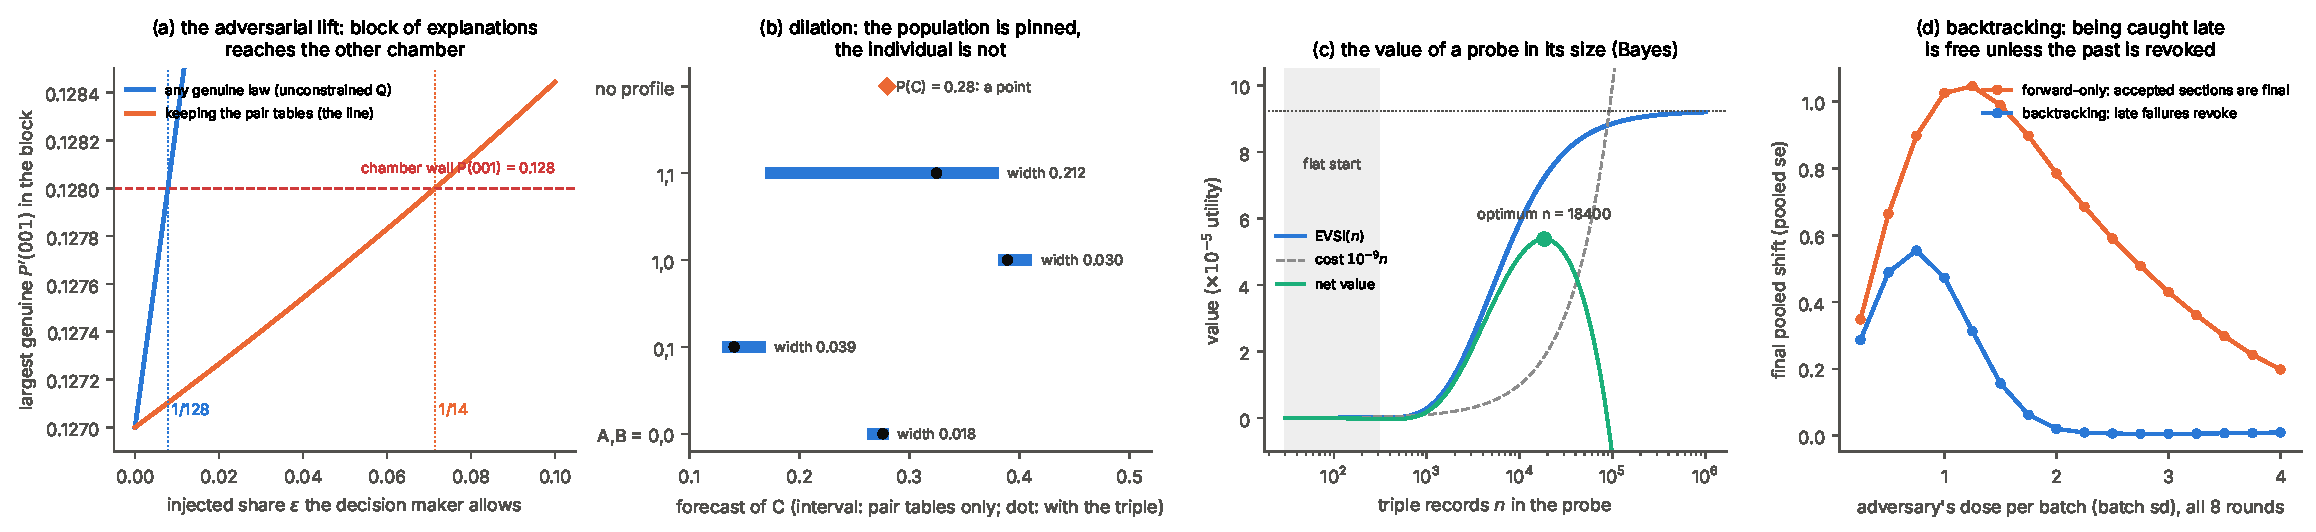
\includegraphics[width=\linewidth]{fig_lifting.pdf}
\caption{Lifting. (a) The adversarial lift on the worked example: the largest $P'(001)$ among genuine laws the data cannot exclude, as
the injected share grows, without constraint and keeping the pair tables. The block reaches the chamber wall $0.128$ at $1/128$ and at
$1/14$. (b) Dilation: pair tables pin $P(C)$ (a point), while the individual forecasts are intervals; the triple's values are marked.
(c) The value of a probe in its size: the flat start, the inflection and the optimal size at a cost of $10^{-9}$ per record. (d)
Backtracking: the final pooled shift against the adversary's dose, for forward-only acceptance and for backtracking.}\label{fig:lifting}
\end{figure}

\section{One picture: chambers, slices and gauges}\label{sec:capstone}
Theorems A--K were proved one at a time. This section states what they have in common. Every quantity in the paper is a question about
how a cover's slices, and a gauge's capacities, meet a chamber arrangement on the fibre.

\paragraph{The objects.}
\begin{itemize}
\item The \emph{fibre} $F$ is the polytope of laws with the observed pair tables (the pair cover). Its \emph{model part}
  $\mathcal M\subseteq F$ is the set of two-type laws in $F$, which is the hiding segment at $m=3$ (\cref{thm:A}).
\item A \emph{decision} is a finite set of linear functionals $\ell_j$ of the law, with walls $\{\ell_j=c_j\}$: $\ell=U_a-U_b$
  with $c=0$, or $\ell=U_a$ with $c=u_0$. The walls cut $F$ into \emph{chambers}.
\item A \emph{probe} refines the cover. With exact data it cuts $\mathcal M$ into \emph{slices} $S_y$. A plateau probe has $S_y=\mathcal M$,
  and the triple has point slices.
\item A \emph{gauge} is a convex set $\mathcal Q$ of admissible injected laws, with support function $h_{\mathcal Q}(\ell)=\sup_{Q\in\mathcal Q}\ell(Q)$:
  \begin{itemize}
  \item the simplex: any record;
  \item $F$ itself: pair tables kept;
  \item the laws that pass the gluing tests of a labelled cover: sources and batches.
  \end{itemize}
\item The \emph{margin} of a law $P$ to a wall is $\delta=c-\ell(P)$, taken positive on the side being approached.
\end{itemize}

\begin{theorem}[one picture]\label{thm:L}
Two latent types, the pair cover. Parts (1), (2) and (5) are for $m=3$, where $F$ is a line. Parts (3) and (4) hold for every $m$.
\begin{enumerate}
\item[(1)] \emph{Settling.} The pre-probe set rule chooses the oracle act at every truth in $\mathcal M$ if and only if $\mathcal M$ lies in
  one chamber.
\item[(2)] \emph{Value of information is slice--chamber incidence.} With exact data, the Savage value of a probe is
  $R(\mathcal M)-\max_yR(S_y)$, where $R(S)=\min_a\max_S\text{regret}_a$. So it equals $R(\mathcal M)$, which is positive exactly when
  $\mathcal M$ meets two chambers, if every slice lies in one chamber, and it is $0$ on a plateau. The Wald value is
  $\min_yW(S_y)-W(\mathcal M)\ge0$, where $W(S)=\max_a\min_SU_a$. For point slices it is positive \emph{if and only if} a wall
  meets the interior of $\mathcal M$ and the two acts' slopes along $F$ are strictly opposite. This is \cref{thm:C}'s saddle-point
  condition read off the chambers.
\item[(3)] \emph{Robustness is margin over capacity.}
  \begin{itemize}
  \item[(a)] \emph{Forward} (from the truth, gauge $\mathcal Q$): the smallest injected share that crosses the wall is
    \[
    \varepsilon=\delta\big/\bigl(h_{\mathcal Q}(\ell)-\ell(P)\bigr).
    \]
    For the simplex the capacity is $\max_x\ell(\delta_x)-\ell(P)$: the vertex attack, exact for linear $\ell$ (\cref{thm:E}(3)). For
    $F$ it is a linear programme, and at $m=3$ it is $s_\pm|\ell(\chi_T)|$: the hidden channel (\cref{thm:F}).
  \item[(b)] \emph{Observer} (from the data): the radius of the block of explanations (\cref{thm:K}(4)) is a water-filling. It removes
    the observed mass from the cells of lowest $\ell$ first, and it equals $\delta/(c-\min_x\ell(\delta_x))$ when the lowest cell holds
    the removed mass. Requiring the genuine law to lie in $\mathcal M$ can only raise it. On the line it is
    $|s'|/(\mathrm{cap}(O)+|s'|)$, where $s'=\delta/\ell(\chi_T)$.
  \item[(c)] \emph{Sampling}: the decision settles half the time at $n_{1/2}=(z\sigma_\ell/\delta)^2$, where $\sigma_\ell$ is the
    per-record standard deviation of the estimate of $\ell$. This is \cref{thm:D}(4) with $d=\delta/|\partial\ell/\partial r|$.
  \item[(d)] \emph{Labelled cover}: a source of share $\pi$ that stays unexposed can move $\hat\ell$ by at most
    $B\sigma_\ell/\sqrt N$, with $B=(c_s-q_\beta)\sqrt{\pi/(1-\pi)}$. Its capacity is measured in standard errors (\cref{thm:J}).
  \end{itemize}
\item[(4)] \emph{Contextuality matters exactly along wall normals.} Whole-record injection keeps the unlabelled cover gluable
  ($\lambda^*=1$, \cref{thm:E}(1)) and moves the law inside $F$. On the labelled cover a contaminated section fails to glue, with
  $1-\lambda^*\ge|\Delta\varepsilon|\,\mathrm{TV}$ (\cref{thm:J}(1)). A failure in direction $\xi$ changes wall $j$ at rate
  $\ell_j(\xi)$. It is \emph{decision-relevant if and only if} $\ell_j(\xi)\ne0$; otherwise no injection along $\xi$, at any share,
  changes the act.
\item[(5)] \emph{Two boundaries.} On $F$ the decision walls and the detection boundary $\partial\mathcal M$ lie on one line (\cref{thm:H}). A
  stealth window $\varepsilon^*<\varepsilon_{\det}$ exists if and only if a wall meets the interior of $\mathcal M$, exactly the
  condition in (1) under which the decision is unsettled.
\end{enumerate}
\end{theorem}

\begin{proof}
(1) If $\mathcal M$ lies in one chamber, some act $a$ dominates on $\mathcal M$, so its worst value is the largest and the set rule picks
it, as the oracle does at every point. If $\mathcal M$ meets two chambers, the oracle act is not constant on $\mathcal M$, while the
set rule's act is.
(2) With exact data the truth lies in its slice and the rule acts on the slice. The worst case over truths is therefore the worst case over
slices of the slice's value, which gives both formulas. For two affine acts $f,g$ on an interval, $W=\max(\min f,\min g)$ and
$W_{\mathrm{post}}=\min\max(f,g)$. If the slopes have the same sign, or one is zero, the upper envelope's minimum is at the same
endpoint as the dominating act's minimum, so the gap is $0$. If they are strictly opposite and cross inside, the upper envelope is
V-shaped with its minimum at the crossing, which is strictly above both acts' minima.
(3a) $\ell\bigl((1-\varepsilon)P+\varepsilon Q\bigr)=\ell(P)+\varepsilon(\ell(Q)-\ell(P))$ reaches $c$ first at the $Q$ maximising $\ell(Q)$.
On the simplex that $Q$ is a vertex. On the $m=3$ line, $\ell(P+s\chi)=\ell(P)+s\,\ell(\chi)$ with $s$ up to the positivity limit.
(3b) $O=(1-\varepsilon)P'+\varepsilon Q$ means that $y=(1-\varepsilon)P'$ is a sub-measure of $O$ of mass $1-\varepsilon$ with
$\ell(y)\ge c\,(1-\varepsilon)$. Maximising the mass is a fractional knapsack, solved by removing mass in increasing order of $\ell$. On
the line both $P'$ and $Q$ move along $\chi$, and $Q\ge0$ bounds $|s_Q|$ by the smallest cell of the relevant sign of $P'=O+s'\chi$.
(3c) The delta method, as in \cref{thm:D}(4). (3d) \Cref{thm:J}(2), applied to $\hat\ell$.
(4) $\ell_j$ is linear. A failure along $\xi$ moves the law by multiples of $\xi$, and the gluable fraction is that of \cref{thm:J}(1).
(5) Moving along $\chi$, the wall is crossed before the end of $\mathcal M$ exactly when it lies inside $\mathcal M$.
\end{proof}

Checks CL1--CL9 (\texttt{engine/check\_capstone.py}) test every part on $150$ random truths and random two-act decisions with utilities
on the eight cells. They also cover the extension of (3a) to $m=4$. There, keeping the pair tables, the support function of the
five-dimensional fibre gives the adversary no more room than at $m=3$, because the fibre's $ABC$ projection lies in the three-variable
fibre ($3.70\%$ both ways). It gives more room than the single $\chi_{ABC}$ channel ($5.05\%$).

\begin{figure}[!htbp]\centering
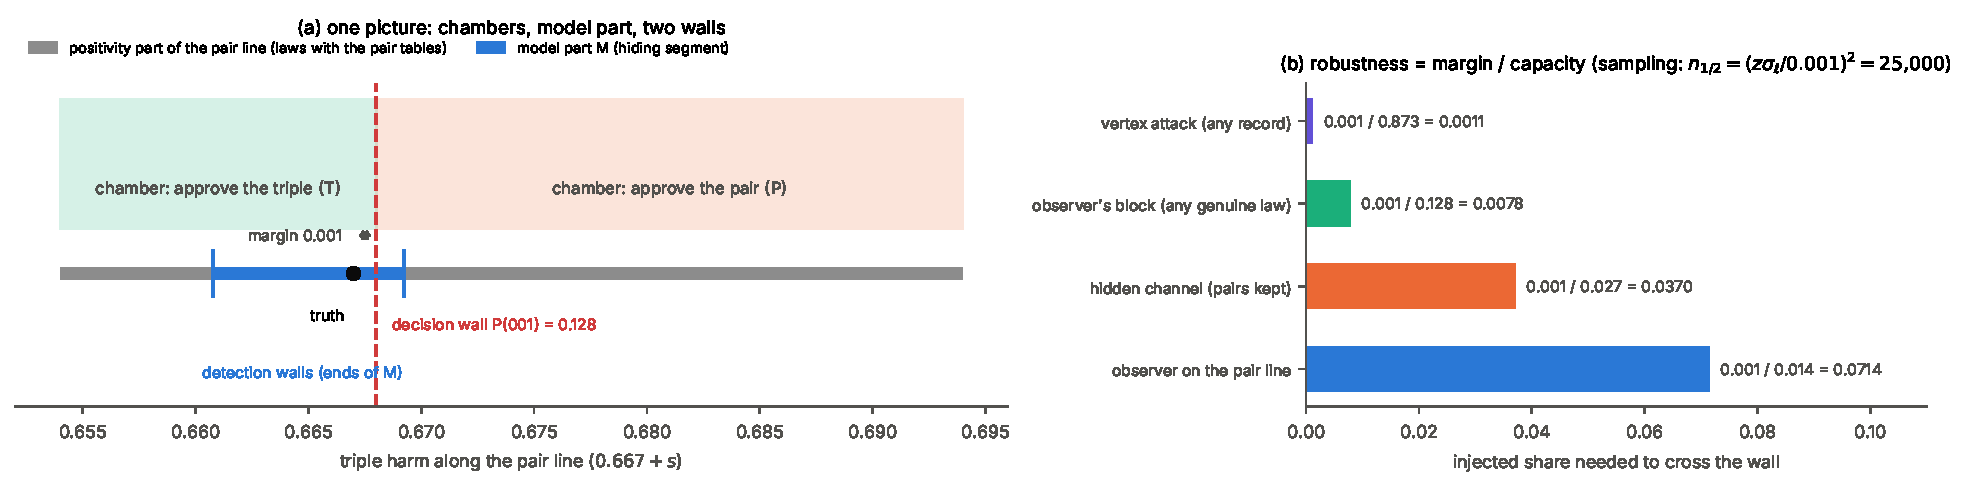
\includegraphics[width=\linewidth]{fig_capstone.pdf}
\caption{\Cref{thm:L} on the worked example. (a) The pair line: the positivity part, the model part $\mathcal M$ with its two detection
walls, and the decision wall $P(001)=0.128$, $0.001$ from the truth. (b) One margin, four capacities: any record, any genuine law,
pairs kept, and the observer on the line. Sampling is the same ratio with a standard deviation as capacity.}\label{fig:capstone}
\end{figure}

\paragraph{The worked example in one line.} The margin is $0.001$ in every reading, and only the capacity changes:
\begin{itemize}
\item any record: $0.873$, so $0.11\%$;
\item any genuine law the data cannot exclude: $0.128$, so $1/128$;
\item pairs kept: $0.027$, so $3.7\%$ (\cref{thm:F});
\item the observer on the line: $0.014$, so $1/14$;
\item sampling: $\sigma_\ell$, so $n_{1/2}=25{,}000$ (\cref{thm:D});
\item a labelled source: $B$ standard errors, so the delay of Study 13.
\end{itemize}
The value of information, the poisoning budgets, the settling size and the bands of Part II are one geometric fact. A wall sits
$0.001$ from the truth, inside the hiding segment, and each question measures that distance in its own gauge.

\paragraph{How far this goes.} \Cref{thm:L} is proved for two types on the pair cover, parts (1), (2) and (5) at $m=3$.
\begin{itemize}
\item Parts (3) and (4) use only linearity and hold on any fibre.
\item With more types, $\mathcal M$ becomes a higher secant variety. It is no longer convex, so (1) needs ``connected component of a
  chamber'', and (2)'s slices are no longer intervals.
\item With other covers, $F$ is a different fibre polytope, but (3) and (4) are unchanged.
\item Non-linear criteria (a risk measure in place of expected utility) curve the walls, and (3a) becomes a support-function inequality
  rather than an equality.
\end{itemize}
The evidence is two worked truths, a few designed ones, and random decisions on three variables. The reach beyond that is open.

\section{The descent tower}\label{sec:descent}
\Cref{thm:L} reads every quantity off one fibre. This section builds the object the fibre is a fibre \emph{of}. It is a diagram of local
spectra over the contexts, together with a descent complex at each level of the tower, and it says which level carries which
obstruction. We stay with ordinary spaces and complexes. Categorification is deferred until this layer is explicit, and the end of the
section names the first place it is forced.

\paragraph{Contexts and local spectra.} Let $V=\{1,\dots,m\}$ be binary variables. The \emph{context category} $\mathcal C$ has the
observed windows $S\subseteq V$ and all their intersections (the empty context included) as objects, with an arrow $S\to T$ when
$T\subseteq S$. For each context let
\[
R_S=\mathbb R[p^S_x:x\in\{0,1\}^S]/(\textstyle\sum_xp^S_x-1),\qquad X_S^{\mathrm{alg}}=\operatorname{Spec}R_S,
\]
the affine space of signed laws on $S$, and let $X_S^{\ge0}$ be its real points with $p\ge0$, the probability simplex.
Marginalisation $\rho_{S,T}$ is a linear map, so it induces ring maps $R_T\to R_S$, and $\rho_{T,U}\circ\rho_{S,T}=\rho_{S,U}$. This
gives a diagram $S\mapsto X_S$ over $\mathcal C$. Its limit is $\operatorname{Spec}$ of the colimit of the rings: families of local
laws whose marginals agree on every overlap. The model layer adds the two-type equations on top. Real probability points and the full
algebraic spectrum are kept apart throughout, because they behave differently.

\begin{proposition}[spectrum and descent]\label{prop:spectrum}
For the pair cover with $m=3$ or $4$, and for the triple cover with $m=4$:
\begin{enumerate}
\item[(1)] \emph{Algebraic descent holds up to a kernel.} The marginal map $X^{\mathrm{alg}}_V\to\lim_{\mathcal C}X^{\mathrm{alg}}_S$ is
  surjective. Its kernel is spanned exactly by the Walsh characters $\chi_S$ of the sets $S$ contained in no window: dimension $1$
  for the pair cover at $m=3$, $5$ at $m=4$, and $1$ for the triple cover. So the presheaf of signed laws satisfies gluing but is not
  separated, and its fibres are torsors under this kernel. The ambient fibre $F$ of \cref{thm:L} is such a torsor cut by positivity.
\item[(2)] \emph{The linear descent complex is acyclic.} For the Čech complex of signed measures on these covers, $H^q=0$ for
  $q\ge1$. Nothing obstructs descent algebraically.
\item[(3)] \emph{Real descent fails only through positivity.} On real points the limit is the local polytope (consistent pseudo-marginals),
  and the image of the simplex is the marginal polytope. When the nerve has a cycle these differ, and the difference is the contextual
  families. Example: $A=B$, $B=C$, $A\ne C$ with uniform margins. It has zero Čech energy, extends to a signed law with least negative
  mass $1/2$, and has $\lambda^*=0$: it is strongly contextual. The certificate is the dual witness of the gluing linear programme, a
  Bell-type inequality, and it is not a cohomology class.
\end{enumerate}
\end{proposition}

\begin{proof}
(1) A signed law on $V$ has the marginals of a consistent signed family whenever the family is consistent. Build it from the
Efron--Stein components of the windows, as \texttt{signed\_extension} in \cite{PG} does. Hence the map is onto $\ker d^0$. A vector is
killed by every window marginal exactly when all its Walsh coefficients on covered sets vanish. (2) and (3) are computed in DC1--DC3.
That the real limit is the local polytope and the image is the marginal polytope is the definition of each.
\end{proof}

\begin{remark}[three cases, and contextuality]\label{rem:threecases}
The descent picture separates three situations, and only the middle one is contextuality in the sheaf-theoretic sense of
\cite{AbramskyBrandenburger2011}: local tables that agree on every overlap but come from no joint law.
\begin{enumerate}
\item \emph{Incongruence.} The tables disagree on an overlap, and the Čech energy (a coboundary) is non-zero. This is inconsistent data,
  not contextuality. The worked example's conflicting trials (\cref{sec:example}, Step 5) are of this kind: energy $0.061$, B margins
  $0.26$ against $0.40$, and $\lambda^*=0.86$.
\item \emph{Contextuality.} The tables agree on every overlap but do not glue. A signed joint law always exists, so linear algebra
  cannot see this case; only positivity fails.
\item \emph{Gluing.} A joint law exists, as for every whole-record injection in Part II ($\lambda^*=1$, \cref{thm:E}(1)).
\end{enumerate}
The family $A=B$, $B=C$, $A\ne C$ (the three-variable liar cycle) is the extreme of case 2.
\begin{itemize}
\item It is \emph{strongly} contextual: $\lambda^*=0$, so no fraction of it is explained by a joint law, and the contextual fraction
  $1-\lambda^*$ is $1$.
\item Any assignment of $A,B,C$ satisfies at most two of the events $A=B$, $B=C$, $A\ne C$, since the first two force $A=C$. So every
  joint law obeys
  \[
  P(A=B)+P(B=C)+P(A\ne C)\le2 .
  \]
  The liar cycle gives $3$, the largest possible violation. The dual witness of the gluing linear programme is an inequality of this
  kind.
\item The least negative mass of a signed extension is $1/2$: the ``negative probability'' reading of the same contextuality.
\item It needs a cycle in the cover. On a tree-shaped cover (for example $AB$, $BC$), consistent tables always glue.
\end{itemize}
For the lab, this means pooled-data adversaries cannot produce contextuality. Injection of whole records keeps $\lambda^*=1$, so
contextual data points to separate populations or to window-by-window manipulation, not to a hidden channel. Contextuality is the
level-0 obstruction and needs no model. The sign of $\Delta_m$ and the tetrads are obstructions only relative to the two-type model
(\cref{thm:M}). All of this is checked in DC3 and DC14.
\end{remark}

So the proposition the attached note proposed, ``global compatible sections coincide with the joint laws'', holds only on the algebraic
spectrum modulo the kernel. On probability points it fails by exactly the contextuality the parent note measures. That failure is
positivity, not cohomology, which is why the parent note needed $\lambda^*$ and not only Čech classes.

\paragraph{The latent layer.} The two-type model writes the pair covariances as $M_{ij}=v_iv_j$. On the graph $\Gamma$ of observed
pairs this is a \emph{multiplicative} 1-cochain, with the unsigned coboundary
\[
\delta^+:C^0(\Gamma;\mathbb R^\times)\to C^1(\Gamma;\mathbb R^\times),\qquad (\delta^+v)_{ij}=v_iv_j .
\]
Split $\mathbb R^\times=\{\pm1\}\times\mathbb R_{>0}$. On signs, written additively in $\mathbb Z/2$, $\delta^+$ is the ordinary
coboundary, since $+1=-1$. On moduli, after taking logarithms, it is the unsigned incidence matrix $B$ of $\Gamma$.

\begin{theorem}[the descent tower]\label{thm:M}
Two latent types.
\begin{enumerate}
\item[(1)] \emph{Level 1, kernel: label switching is non-separatedness.} $\ker(\delta^+)$ on signs is $H^0(\Gamma;\mathbb Z/2)=\mathbb Z/2$
  for connected $\Gamma$: the switch $v\mapsto-v$, which with $r\mapsto-r$ exchanges the types. On moduli the kernel is $0$ if
  $\Gamma$ is connected and not bipartite (the triangle, $K_4$). It is $1$-dimensional if $\Gamma$ is bipartite (the path
  $AB,BC$): there the scale of $v$ is not pinned, which is the blow-up direction of \cref{thm:K}(3).
\item[(2)] \emph{Level 1, obstruction.} Pair tables have the algebraic form $M=\delta^+v$ if and only if two classes vanish:
  \begin{itemize}
  \item the \emph{sign class} in $H^1(\Gamma;\mathbb Z/2)$, whose cycle parities are the signs of $\prod_{\text{cycle}}M_{ij}$;
  \item the \emph{modulus class} in $\operatorname{coker}B$.
  \end{itemize}
  On the triangle the sign class is $\operatorname{sign}(M_{01}M_{02}M_{12})=\operatorname{sign}(\Delta_m)$, the ladder's rung, and
  $\operatorname{coker}B=0$, so three variables carry no equation. On $K_4$ the sign classes form $H^1(K_4;\mathbb Z/2)=(\mathbb Z/2)^3$,
  and $\operatorname{coker}B$ is $2$-dimensional and spanned by the two log tetrad ratios. \emph{The tetrads are the modulus class.}
  Algebraically, the ideal of the image of $v\mapsto(v_iv_j)$ is the toric ideal of $B$: zero on the triangle and generated by the two
  tetrads on $K_4$. The number of sign cosets left unreached by real $v$ is $|H^1(\Gamma;\mathbb Z/2)|$.
\item[(3)] \emph{Level 1, walls.} Beyond both classes, a two-type explanation needs the box walls to leave a non-empty segment. This is a
  semialgebraic condition, not a cohomological one. With three variables, pair tables are two-type realizable if and only if the sign
  class vanishes and the walls leave a segment.
\item[(4)] \emph{Level 2, triple coherence.} On the triple cover, $r_S=m_S/v_S$ is a 0-cochain, and the model requires it to be
  constant: $\delta r=0$, with the quadruple window adding $m_{0123}=v_{0123}(r^2+1)$. A single-triple channel $\chi_S$ leaves levels 0
  and 1 unchanged, because it has the same pair tables, and makes $\delta r\ne0$ at first order. The obstruction moves up exactly one
  level, which is why a second triple detects what no pair check can (\cref{cor:secondtriple}).
\item[(5)] \emph{The fibre.} At $m=3$ the level-0 torsor over the data (the line $P+s\chi_T$) meets the level-2 condition ($\hat r$
  inside the walls) exactly in the hiding segment.
\item[(6)] \emph{Labels: a degree-0 obstruction.} On the labelled cover the batches pairwise overlap in the whole triple context, so
  the nerve is a simplex and $H^q=0$ for $q\ge1$. The shared statistic $m_T$ is a 0-cochain, and one population means it lies in $\ker\delta^0$
  (constants). The obstruction to a common realization is therefore the coboundary $\delta^0m_T\in B^1\cong\mathbb R^K/\mathbb R$ of
  dimension $K-1$, in the group $\mathbb R\chi_T$ of the hidden channel. It is a failure of overlap compatibility, \emph{not} an $H^1$
  class. Its energy splits orthogonally as
  \[
  \|\delta^0m_T\|^2=K\bigl(\text{between-source}+\text{within-source}\bigr),
  \]
  and these are the coarse and the fine covers of the gluing filter. \Cref{thm:J}'s source statistic is the normalised between-source
  contrast. Its decision-relevant part is $\ell(\chi_T)\,\delta^0m_T$ (\cref{thm:L}(4)). Pooling is the monad multiplication, which
  forgets $\delta^0$, and the band of \cref{thm:J} is how much of $\delta^0m_T$ the noise can hide.
\item[(7)] \emph{What the realization diagram remembers.} Every $2\times2$ table is a mixture of two product laws on its own, so the
  diagram of \emph{images} (locally two-type laws) has the same limit as level 0. On the triangle, a law with $\Delta_m<0$ has pair
  tables that glue and are each two-type, yet admit no global two-type realization. Only the diagram of \emph{realizations}
  $S\mapsto\{(v_i)_{i\in S}\}$ sees this. Its limit is the set of global realizations, and its emptiness is measured by
  \[
  H^1_+(\Gamma;\mathbb R^\times)=C^1/\delta^+C^0\cong H^1(\Gamma;\mathbb Z/2)\oplus\operatorname{coker}B,
  \]
  which is $\mathbb Z/2$ on the triangle and $(\mathbb Z/2)^3\oplus\mathbb R^2$ on $K_4$. The ladder's rung and the tetrads are the
  two summands. The gluing of images is ordinary; realizability is not.
\end{enumerate}
\end{theorem}

\begin{proof}
(1) Over $\mathbb Z/2$, $\delta^+$ is the graph coboundary, whose kernel is the locally constant functions. Over $\mathbb R$, the
unsigned incidence matrix of a connected graph has rank $m$ if the graph is not bipartite, and $m-1$ if it is. (2) $M=\delta^+v$ splits
into $\operatorname{sign}M=\delta(\operatorname{sign}v)$ and $\log|M|=B\log|v|$, and each is solvable exactly when the right side is in
the image. On a cycle the sum of the sign cochain is the parity of $\prod M_{ij}<0$. The toric ideal of $B$ cuts out the Zariski closure
of the image (DC7). (3) Two types exist when $v$ exists and some $t$ makes $(w,a_1,a_2)$ valid, which is the segment condition (DC9).
(4) $\chi_S$ changes no pair table and moves $m_S$ alone, by $2^{m-3}\varepsilon s$ (\cref{thm:F}(4)). (5) Check DC11. (6) The nerve of a cover in which every finite intersection is non-empty is a full simplex, which is contractible. $\sum_{b<c}(m_c-m_b)^2=K\sum_b(m_b-\bar m)^2$, and the total sum of squares splits into between- and within-source parts (DC12). (7) A $2\times2$ table is the mixture of its two rows, each a product law; the counterexample is DC13, and the isomorphism is (2).
\end{proof}

\begin{corollary}[the descent filtration]\label{cor:filtration}
On pair data, together with triple windows when they are observed, set
\begin{itemize}
\item $D_0$: compatible families;
\item $D_1\subseteq D_0$: families that glue (the marginal polytope);
\item $D_2\subseteq D_1$: sign class $0$;
\item $D_3\subseteq D_2$: modulus class $0$;
\item $D_4\subseteq D_3$: the walls leave a segment;
\item $D_5\subseteq D_4$: triple coherence $\delta r=0$.
\end{itemize}
Each inclusion is strict. The witnesses are:
\begin{itemize}
\item $D_0\setminus D_1$: the liar cycle;
\item $D_1\setminus D_2$: a joint law with $\Delta_m<0$;
\item $D_2\setminus D_3$: a joint law on four variables with trivial signs and non-zero tetrads;
\item $D_3\setminus D_4$: a joint law with both classes zero and no segment;
\item $D_4\setminus D_5$: a two-type law with a $\chi_S$ channel.
\end{itemize}
These are checked in DC3, DC5, DC10 and DC16. The order of $D_2$, $D_3$ and $D_4$, which puts algebraic before semialgebraic and signs
before moduli, is a convention. The stages are not. What the filtration predicts beyond the moment equations of a given cover is a
general count. For \emph{any} connected pattern of observed pairs with $E$ edges on $m$ variables:
\begin{itemize}
\item the two-type model imposes exactly $E-\operatorname{rank}B$ equations on the pair moments: $E-m$ when the graph is not
  bipartite, $E-m+1$ when it is;
\item there are $b_1=E-m+1$ independent sign conditions;
\item exactly $2^{-b_1}$ of the sign patterns are reachable.
\end{itemize}
This is checked against Jacobian ranks on $57$ random graphs (DC15).
\end{corollary}

\begin{table}[!htbp]\centering\small
\begin{tabular}{p{0.15\linewidth}p{0.22\linewidth}p{0.23\linewidth}p{0.28\linewidth}}\toprule
level & kernel (non-separatedness) & obstruction & certificate\\\midrule
0: ambient laws & Walsh characters of uncovered sets (the fibre's directions) & none algebraically; positivity on real points & LP witness (Bell-type inequality), $\lambda^*$\\
1: pair layer, signs & $\mathbb Z/2$: the label switch & $H^1(\Gamma;\mathbb Z/2)$ & $\operatorname{sign}\Delta_m$ on each cycle\\
1: pair layer, moduli & $0$ (non-bipartite) or scale (bipartite) & $\operatorname{coker}B$ & tetrads ($m\ge4$)\\
1: walls & --- & positivity & the segment is empty\\
2: triple layer & --- & $\delta r\ne0$ & a second triple; the quadruple equation\\
labels (degree 0) & --- & $\delta^0m_T\ne0$ across batches & the gluing tests of \cref{thm:J}\\\bottomrule
\end{tabular}
\caption{The descent tower: what each level fails to separate, what obstructs descent there, and what certifies the obstruction
(checks DC1--DC16).}\label{tab:tower}
\end{table}

\paragraph{Where categorification is forced.} The first genuinely categorical step is already in (1)--(2). Two local realizations on an
overlap agree only up to the label switch. So the realizations form a groupoid, the quotient stack $[\Theta_S/(\mathbb Z/2)]$, not a set,
and the sign class is the class of the gluing data in Čech $H^1$ with coefficients in the automorphism group $\mathbb Z/2$. A global
realization exists when this $\mathbb Z/2$-torsor on $\Gamma$ is trivial. This is the precise sense in which the latent layer needs
realization \emph{spaces} rather than sets. Higher stacks, hypercovers and operadic realization would enter only with more types: there
the automorphisms permute $k$ types, the coefficient group becomes the symmetric group $S_k$, and the cohomology is non-abelian. We leave
that open.

\paragraph{Two comonads.} Two different comonads appear in this paper, and they should not be confused.
\begin{itemize}
\item The \emph{provenance comonad} $W=L\times(-)$ (\cref{sec:inj,sec:sources}) is the environment comonad of a set $L$ of labels
  (source, batch). Its counit $\varepsilon:L\times X\to X$ forgets the label, and its comultiplication copies it. Its co-Kleisli maps
  $L\times X\to A$ are the \emph{label-aware decision rules}. A rule that pools factors through $\varepsilon$; the gluing filter of
  \cref{thm:J} does not. The counit of a comonad always satisfies the comonad laws, so ``detection'' is never a failure of the counit. It
  is the gap between a co-Kleisli rule and its factorisation through $\varepsilon$.
\item The \emph{cover comonad} belongs to a cover $f:\coprod_iU_i\to X$. Write $f^*$ for restriction to the pieces and $f_*$ for its
  right adjoint, so $f^*\dashv f_*$. The adjunction has a unit $\mathrm{id}\Rightarrow f_*f^*$ on the side of $X$ and a counit
  $f^*f_*\Rightarrow\mathrm{id}$ on the side of the cover. The comonad is therefore $G=f^*f_*$, and it acts on presheaves over the
  \emph{cover} $\coprod_iU_i$, not over $X$. Its counit is the counit of the adjunction, and its comultiplication is
  $f^*(\text{unit})f_*$. Its coalgebras are the descent data of the cover \cite{BenabouRoubaud1970,JanelidzeTholen1994}. The monad
  $f_*f^*$ on the side of $X$ is the other half of the same adjunction, and its cosimplicial resolution is the Čech complex of
  (i) below. This is the comonad of the descent tower.
\end{itemize}
The two meet in the labelled cover of \cref{thm:J}. There the batches are the pieces of the cover, so the label set $L$ indexes the
cover's pieces. Pooling is the multiplication $\mu:D(DX)\to DX$ of the distribution monad $D$ \cite{Giry1982}, and the gluing
condition is that the family of batch laws lies in the image of the unit $\eta$ (\cref{sec:sources}).

\begin{proposition}[the comonadic form of the descent tower]\label{prop:comonadic}
Let $\mathcal U=\{U_i\}$ be the cover by observed windows, and let $K$ send a joint law (signed, or a probability law) to its family of
window marginals.
\begin{enumerate}
\item[(i)] \emph{Comonadic realization of descent.} The cosimplicial resolution of the cover comonad has $n$-th term
  $\prod F(U_{i_0}\cap\dots\cap U_{i_n})$ over all ordered $(n+1)$-tuples, repetitions included. Its unnormalised cochain complex has
  the same cohomology as the alternating Čech complex of \cref{prop:spectrum}, because the degenerate part is acyclic. On the pair cover
  the unnormalised complex has dimensions $12,24,54,\dots$ and cohomology $7,0,0$, as the alternating one does (check DC17). So the lab's
  Čech complex \emph{is} the normalised classical comonadic resolution; no new comparison construction is involved. For a single presheaf
  $F$, the descent data of $\mathcal U$ are the equalizer $\ker d^0$ of this resolution, and $K:F(X)\to\ker d^0$ is the comparison map
  at $F$. Descent at $F$ (the sheaf condition: separated and gluing) means that $K$ is a bijection.
\item[(ii)] \emph{Three distinct failures of $K$.}
  \begin{enumerate}
  \item[(a)] \emph{Injectivity fails.} $\ker K$ is spanned by the Walsh characters of the uncovered sets, which is the hiding fibre and
    the hidden channel. This is a loss of identifiability. By itself it is not contextuality.
  \item[(b)] \emph{Surjectivity fails, through positivity only.} On signed laws $K$ is onto $\ker d^0$ and the resolution is acyclic in
    degrees $\ge1$. This is proved for the lab's covers, not assumed. On probability laws, $K$ misses exactly the contextual families.
    That failure is decided by a feasibility linear programme and its dual witness, and not by a cohomology class of either natural
    linearisation (\cref{prop:csd}(1)).
  \item[(c)] \emph{Latent descent fails with automorphisms.} Two-type realizations form a groupoid whose automorphisms are the label switch
    $\mathbb Z/2$. Descent for groupoid-valued data is governed by non-abelian Čech $H^1$ with coefficients in the automorphisms, and
    here the obstruction is a class in $H^1(\Gamma;\mathbb Z/2)$, the sign of $\Delta_m$ (\cref{thm:M}(2)). It is distinct from (a) and (b):
    a law can glue and still carry this class (the ``exactly one harm'' law of Step~14).
  \end{enumerate}
\item[(iii)] \emph{The source-labelled discrepancy.} On the labelled cover the triple-moment discrepancy is the degree-$0$ coboundary
  $\delta^0m_T$ on a simplex nerve (\cref{thm:M}(6)); it is not an $H^1$ class. On the unlabelled cover, whole-record injection stays in the
  image of $K$ ($\lambda^*=1$), so the discrepancy is invisible there. On the labelled cover, assume two things: every batch's
  tables arise from an actual batch law (a probability law on all $m$ variables), which is the case under whole-record injection; and
  $\delta^0$ vanishes on every window, so that all batches agree on every table. Then the common compatible family is realised by any
  one batch law. It is therefore the image under $K$ of a genuine probability law, not merely of a signed solution: positivity comes for
  free under these two assumptions, and only under them. At $m=3$, in addition, the batch laws themselves coincide. On three binary
  variables the $8$ cells have $7$ free coordinates, and the singles, the pairs and $m_T$ supply exactly $7$ that determine the law (the
  moment normal form of \cite{PG}). Vanishing does not place the common law in the two-type model; that needs stages $D_2$--$D_5$ (\cref{cor:filtration}). In data
  $\delta^0m_T$ is never exactly zero, and ``vanishing'' means passing the tests of \cref{thm:J}.
\end{enumerate}
\end{proposition}

\begin{proof}
(i) The resolution of $G$ applied to $F$ is the Čech nerve of the cover evaluated in $F$
\cite{Godement1958,JanelidzeTholen1994}. Normalisation, which quotients by degeneracies, preserves cohomology
\cite{Weibel1994}, and the ordered and alternating Čech complexes have the same cohomology \cite{Godement1958}. The numbers are DC17. The
equalizer of the first two coface maps consists of the families that agree on overlaps. (ii)(a), (b): \cref{prop:spectrum} and
\cref{prop:csd}. (ii)(c): \cref{thm:M}. The ``exactly one harm'' law is a probability law, so it glues, and its class is DC5 and WD5.
(iii) If all batches agree on every window, any one batch's law realises the common family. At $m=3$ the law is a polynomial function of
singles, pairs and $m_T$ (the moment normal form of \cite{PG}).
\end{proof}

\paragraph{How each classical theorem applies.}
\begin{itemize}
\item \emph{Eilenberg--Moore} \cite{EilenbergMoore1965}. Every adjunction $f^*\dashv f_*$ gives a comonad $G=f^*f_*$ on presheaves over the
  cover and a monad $f_*f^*$ on the side of $X$, each with its category of (co)algebras and a comparison functor
  from presheaves on $X$. In the lab, $f^*$ restricts a presheaf on all contexts to the windows, and the coalgebras are
  families of window data with restriction-compatible structure.
\item \emph{Bénabou--Roubaud} \cite{BenabouRoubaud1970}. For a bifibration satisfying the Beck--Chevalley condition, the descent data
  along $f$ are exactly the (co)algebras of the induced (co)monad. This is what licenses calling the families that agree on overlaps
  ``coalgebras'': the lab's restriction maps are marginalisations, which compose and commute with restriction to sub-contexts. The lab
  uses only its object-level consequence, that descent data are the equalizer of the resolution.
\item \emph{Beck's comonadicity theorem} \cite{Beck1967,MacLane1998}. $f^*$ is comonadic, so that the comparison functor is an
  equivalence and $f$ is an effective descent morphism \cite{JanelidzeTholen1994}, if and only if $f^*$ reflects isomorphisms and
  preserves the relevant equalizers. The lab works with one presheaf at a time, so it sees the object-level counterparts of Beck's two conditions. (ii)(a) is
  a failure of separation: $K$ identifies laws that differ by $\chi_S$, which is the object-level shadow of not reflecting
  isomorphisms. (ii)(b) shows that, even where the linear comparison is onto, the probability comparison is not. At the level of these
  presheaves, then, the window cover does not give effective descent, and (ii) names the two reasons. We do not claim a statement about
  the comparison functor on all presheaves.
\item \emph{Godement} \cite{Godement1958}. The cosimplicial resolution of a comonad computes Čech (and derived) cohomology, and the
  ordered, alternating and normalised versions agree. This is (i), checked numerically in DC17.
\item \emph{Normalisation and Dold--Kan} \cite{Weibel1994}. For cosimplicial abelian groups, the normalised complex is chain-homotopy
  equivalent to the unnormalised one. This is why the paper's alternating Čech complex can stand for the comonadic resolution.
\item \emph{Non-abelian $H^1$} \cite{Giraud1971}. Gluing groupoid-valued data up to their automorphisms is classified by $H^1$ with
  coefficients in the automorphism sheaf. In the lab this is the $\mathbb Z/2$ of the label switch, giving (ii)(c). With $k$ types the
  coefficients become the symmetric group $S_k$.
\end{itemize}
The lab's contribution is therefore not a new equivalence between comonadic descent and Čech cohomology. It is the explicit separation
and calculation, inside one realization problem, of four phenomena: the kernel, positivity, provenance, and the latent automorphisms. It
also pins down the degree and the meaning of the source-labelled discrepancy.

\section{Relation to the CSD framework}\label{sec:csd}
The Categorified Spectral Duality (CSD) programme \cite{ChangCSD2026} builds, for an admissible operator-semantic system
$A=(\mathcal O_A,\mathcal C_A,\tau_A,\rho_A)$, a spectral stack $\operatorname{Spec}(A)$ by operadic syntactic realization, a left Kan
extension and hypersheafification. It then defines an obstruction cohomology $\mathrm{Obs}^\bullet(A)=H^\bullet(\operatorname{Spec}(A),F^{\mathrm{lin}}_A)$
from a descent filtration, and assigns contextuality to degrees through $\operatorname{CtxSpec}(A)=\{n:\mathrm{Obs}^n(A)\ne0\}$.
Several of its results are stated under hypotheses (geometricity, perfectness, reconstruction, hyperdescent, full faithfulness). Some
computations are deferred to future work, including the linearised sheaf $F^{\mathrm{lin}}_A$ for its examples.

We do not import that machinery. The lab is a classical, commutative setting with no operad, so $\operatorname{Spec}(A)$ is not
constructed here. What the lab does supply are the data the two frameworks share:
\begin{itemize}
\item a context category: the windows and their intersections;
\item a covering: by the windows;
\item a presheaf of local realizations: local laws, or local two-type realizations up to the label switch.
\end{itemize}
On these data we can prove what any Čech-type obstruction theory can and cannot do. This is the connection we can actually establish.

\begin{proposition}[the lab inside CSD: what an obstruction class can see]\label{prop:csd}
On the lab's covers (the pair cover at $m=3,4$):
\begin{enumerate}
\item[(1)] \emph{No linear or support-based class characterises gluing of probability laws.} Let $\theta$ be an invariant of compatible
  families that factors through either
  \begin{itemize}
  \item[(i)] the linear Čech cohomology of signed families, or
  \item[(ii)] the support presheaf (which local outcomes have positive probability).
  \end{itemize}
  Then $\theta=0$ cannot be equivalent to ``the family glues''. For (i), linear Čech cohomology vanishes in every degree $\ge1$ (DC2),
  yet the liar cycle is compatible and does not glue. For (ii), the noisy liar $(1-q)\,\mathrm{liar}+q\,(\text{independent uniform})$ has
  full support for every $q>0$. It is contextual for $0<q<2/3$: $\lambda^*<1$, and the Bell value $3-\tfrac32q$ exceeds $2$. It glues
  from $q=2/3$. So a support-based invariant cannot tell $q=0.3$ from $q=1$. For probability laws, gluing is decided by positivity, a
  linear programme and its dual witness (\cref{rem:threecases}), not by the vanishing of such a class. The CSD statement
  ``$\mathrm{Obs}_{\mathrm{CSD}}(A)=0$ iff every compatible family glues'' can therefore hold for probabilistic models only with a
  linearisation of neither kind. The CSD paper does not construct one, and we do not know whether one exists.
\item[(2)] \emph{Where Čech cohomology on $\Gamma$ does detect, the degree is $1$.} For all-versus-nothing families the supports are affine parity
  conditions. The liar cycle's are $a+b=0$, $b+c=0$, $a+c=1$. Its edge-parity cochain $(0,0,1)$ on the graph $\Gamma$ of windows is not a
  coboundary, which gives a non-zero class in $H^1(\Gamma;\mathbb Z/2)$ \cite{AbramskyMansfieldBarbosa2012}. This is the same group as
  the latent sign class of \cref{thm:M}(2). The nerve of the pair cover is a hollow triangle at $m=3$ (reduced Betti numbers $b_1=1$,
  $b_2=0$), and at $m=4$ it has $b_1=3$, $b_2=b_3=0$. So Čech $H^2$ vanishes on these covers for every coefficient group, and no class
  of degree $\ge2$ arises. Computed on these data, the ``contextuality polynomial'' of the liar cycle is $t$ with $\mathbb Z/2$ support
  coefficients and $0$ with real linear coefficients.
\item[(3)] \emph{The lab's degree-two obstruction is a deformation obstruction, not a gluing obstruction.} The class that \emph{does}
  sit in degree two in the lab is the André--Quillen class $\mathrm{ob}(A)=[\tfrac12H(A,A)]\in\operatorname{coker}J$ of \cref{thm:G}(4).
  It is the obstruction to extending a first-order deformation along the tetrad scheme. This matches CSD's reading of $H^2$ of a tangent
  complex as ``primary obstruction classes'' in deformation theory. In the lab the two obstructions are distinct objects, computed
  separately: gluing in Čech degree $1$, deformation in cotangent degree $2$.
\item[(4)] \emph{What transfers.} CSD's realizations form $\infty$-groupoids. The lab's first genuinely groupoid-valued case is the
  two-type realization stack $[\Theta_S/(\mathbb Z/2)]$ (\cref{thm:M}), whose gluing obstruction is in $H^1(\Gamma;\mathbb Z/2)$ and whose
  automorphisms are the label switch. With $k$ types the automorphism group is the symmetric group $S_k$ and the obstruction becomes
  non-abelian. That is the first place where higher coherence of the CSD kind could appear in the lab. We have not computed it.
\end{enumerate}
\end{proposition}

\begin{proof}
(1)(i) The invariant takes the same value on the liar cycle and on any gluing family, because both have zero class in every degree
$\ge1$. (ii) The noisy liar at $q=0.3$ and $q=1$ have the same supports, all four cells in every window, yet only the second glues. The
numbers are computed in CX4. (2) The parity system is solvable exactly when the cochain is a coboundary (CX3). The Betti numbers are
computed over $\mathbb Z/2$ (CX2). (3) \Cref{thm:G}(4) and check IN11. (4) \Cref{thm:M}.
\end{proof}

\begin{table}[!htbp]\centering\small
\begin{tabular}{p{0.27\linewidth}p{0.36\linewidth}p{0.28\linewidth}}\toprule
CSD notion & lab instance & status\\\midrule
context category $\mathcal C_A$, topology $\tau_A$ & windows and intersections; covering by windows & defined (\cref{sec:descent})\\
sheaf of local realizations $F_A$ & local laws; two-type realizations up to label switch & defined; descent computed (\cref{prop:spectrum}, \cref{thm:M})\\
$\operatorname{Spec}(A)$ via operad, $\mathrm{Lan}$, hypersheafification & not constructed (no operad in a commutative classical setting) & not instantiated\\
$\mathrm{Obs}_{\mathrm{CSD}}=0\iff$ gluing & fails for linear and support linearisations of probability laws & proved (\cref{prop:csd}(1))\\
primary obstruction in degree 2 & gluing obstruction in Čech degree 1; Čech $H^2=0$ on these covers & computed (CX2, CX3)\\
$H^2$ of tangent complex as obstructions & André--Quillen class of \cref{thm:G}(4) & matches\\
realizations as $\infty$-groupoids & the stack $[\Theta_S/(\mathbb Z/2)]$ & first case; $S_k$ case open\\
$\mathrm{Obs}^n$, $n\ge3$ (higher contextuality) & none on these covers & vanish (nerve dimension)\\\bottomrule
\end{tabular}
\caption{The CSD framework on the lab's data (checks CX1--CX5).}\label{tab:csd}
\end{table}

\paragraph{Summary.} On classical probability tables the descent filtration does distinguish real levels (\cref{cor:filtration}, \cref{tab:tower}), but the
obstruction that decides gluing is positivity. It is not a cohomology class of the linear or the support linearisation. Where a Čech class
does decide (the all-versus-nothing families and the latent sign), it sits in degree $1$, in the group $H^1(\Gamma;\mathbb Z/2)$.
Higher Čech degrees do not arise on these covers, and in the lab degree two is the deformation degree. Degrees are not absolute: they
depend on the complex. Roumen's order cohomology places the complete extension obstruction in \emph{relative} degree $2$, via a
connecting map out of degree $1$, and that convention agrees with CSD's (\cref{sec:markov}). A proof that CSD's $\operatorname{Spec}$ restricts to
the lab's diagram would need its construction for commutative classical systems. If such a construction is given, the lab supplies
computed test cases for every invariant above.

\paragraph{Relation to Ikeda's entanglement obstruction.} Ikeda \cite{Ikeda2025} treats entanglement as a cohomological obstruction
in the quantum marginal problem. The setting is a presheaf $S$ of density operators on subsystems, with restriction by partial trace,
and the restriction map $j_{\mathcal U}:S(I)\to H^0(\mathcal U,S)$. The paper names two failure modes: (A) \emph{gluing failure}, when
$j_{\mathcal U}$ is not surjective, and (B) \emph{non-uniqueness}, when it is not injective. These are exactly the lab's failures
(ii)(b) and (ii)(a) of $K$ in \cref{prop:comonadic}. The correspondence is more than an analogy: the lab is the commutative part of
Ikeda's problem.

\begin{proposition}[the lab inside the quantum marginal problem]\label{prop:quantum}
Identify a law on $\{0,1\}^m$ with the diagonal density operator in the product basis.
\begin{enumerate}
\item[(1)] \emph{Dephasing is a retraction.} Full dephasing $\Delta$ in the product basis commutes with every partial trace. So if a quantum
  state $\rho$ has diagonal window marginals, then $\Delta(\rho)$ is a classical law with the same marginals. Hence a diagonal compatible
  family glues quantum-mechanically if and only if it glues classically. The lab's contextual families, the liar cycle among them, are
  gluing failures (A) in Ikeda's sense too.
\item[(2)] \emph{Non-uniqueness grows.} On the three-qubit pair cover, the kernel of the classical $K$ is spanned by $\chi_{ABC}$, which is
  $-Z\otimes Z\otimes Z$ on the diagonal. The kernel of the quantum restriction on Hermitian operators has dimension $27$, spanned by the
  weight-$3$ Pauli strings. Coherences add $26$ directions that no two-qubit window sees, and the lab's hidden channel is the single
  commuting one.
\item[(3)] \emph{Witnesses.} Ikeda's separability witnesses ($\operatorname{Tr}(W\sigma)\ge0$ for all separable $\sigma$, with
  $\operatorname{Tr}(W\rho)<0$ detecting entanglement) and the lab's dual witnesses of the gluing linear programme are both supporting
  hyperplanes of a convex set. They separate a point from the set of realizable states, and this is the positivity side of the
  obstruction in both settings.
\end{enumerate}
\end{proposition}

\begin{proof}
(1) $\Delta$ keeps the diagonal and $\operatorname{Tr}_{C}$ sums diagonal entries over $C$, so $\Delta\circ\operatorname{Tr}_C=\operatorname{Tr}_C\circ\Delta$
(check QU1). If $\rho$ realises the family, so does $\Delta(\rho)$ (QU2). (2) A Pauli string acting non-trivially on all three qubits has
zero partial trace onto any two of them. The $64$-dimensional space of Hermitian operators has $1+9+27+27$ strings by weight; the windows
see weights $0$ to $2$, and the kernel is the $27$ weight-$3$ strings (QU3). (3) Hahn--Banach separation in finite dimensions.
\end{proof}

Ikeda's Theorem~3.1 \cite{Ikeda2025} is a different kind of result, and it should be read as a comparison. For a smooth family of
full-rank states over a parameter manifold $X$, it takes the Uhlmann connection $A$ on the amplitude bundle and a separability-witness
field $W_{\mathrm{sep}}$ that is covariantly constant ($D_AW_{\mathrm{sep}}=0$). The Bott--Shulman--Stasheff--Dupont construction then
gives a Čech--de Rham cocycle whose class is $\bigl[(2\pi i)^{-k}\operatorname{Tr}(W_{\mathrm{sep}}F^k)\bigr]_{\mathrm{dR}}\in H^{2k}_{\mathrm{dR}}(X)$.
For $W_{\mathrm{sep}}=1$ the form $(2\pi i)^{-k}\operatorname{Tr}F^k$ is $(-1)^kk!$ times the $k$-th Chern-character form; it agrees with
a Chern class only after Newton's identities. Its degree is even and positive, and it lives on a parameter space. The lab's obstructions
are different: positivity, degree $0$ ($\delta^0m_T$) and degree $1$ ($H^1(\Gamma;\mathbb Z/2)$). The lab's closest object is the
Kähler class of the toric fibre $\mathbb{CP}^1$ (Step~13). Its area over $2\pi$ is the lattice length $s_++|s_-|=0.040$, which is the
adversary's total capacity on the line. The hidden channel moves the point but leaves that length unchanged (QU4). So the
curvature-type invariant measures the size of the fibre, while the descent and positivity tests decide realizability and where the truth
sits. The two are complementary, and the lab shows it on one example.

\section{Markov categories: factorisation, sufficiency, de Finetti and Blackwell}\label{sec:markov}
Markov categories \cite{Fritz2020} give probability a compositional, diagrammatic foundation. Morphisms are Markov kernels; every
object has a copy map; and conditional independence, sufficiency and almost-sure equality are defined by diagrams. Three theorems of
that programme apply to the lab directly, and a fourth idea, tangent structure, applies at one precise point. Each is shown below on a
small example worked by hand (\cref{fig:markov}, checks MK1--MK6).

\begin{proposition}[the lab in a Markov category]\label{prop:markov}
Work in $\mathsf{FinStoch}$, finite sets and stochastic matrices.
\begin{enumerate}
\item[(1)] \emph{The two-type model is a factorisation.} A law $P$ on $\{0,1\}^3$ is two-type exactly when it factors as
  \[
  I\xrightarrow{\ w\ }Z\xrightarrow{\ \mathrm{copy}\ }Z\otimes Z\otimes Z\xrightarrow{\ K_A\otimes K_B\otimes K_C\ }X_A\otimes X_B\otimes X_C,
  \]
  with $Z$ a two-point object. This says that $A$, $B$ and $C$ are conditionally independent given $Z$. The hiding segment is the set of
  such factorisations with fixed pair marginals.
\item[(2)] \emph{Sufficiency on the line.} For the family $P_s=P+s\chi_{ABC}$, every pair window is ancillary for $s$: its Fisher
  information is $0$. The triple window carries $I(s)=\sum_x\chi(x)^2/P(x)=\sum_x1/P(x)$ at $s=0$. The pair tables are therefore not
  sufficient for the hidden coordinate, which is Fritz's synthetic sufficiency \cite{Fritz2020} read on the fibre.
\item[(3)] \emph{De Finetti for batches.} The batch laws define a mixing measure $\pi=\frac1K\sum_b\delta_{P_b}\in D(DX)$. Records are
  exchangeable across all batches if and only if $\pi$ is a Dirac, and only partially exchangeable (within batches) otherwise; this is the
  de Finetti picture of \cite{FritzGondaPerrone2021,ChenEtAl2025}. Pooling is the multiplication $\mu$, and $\mu(\pi)$ can equal a
  whole-pool injection exactly. The population version of \cref{thm:J}'s test statistic is $\operatorname{Var}_\pi(m_T)$, which is zero
  if and only if $\pi$ is a Dirac.
\item[(4)] \emph{Blackwell.} If an experiment $E_2$ is a garbling of $E_1$ ($E_2=E_1G$ for a stochastic $G$), then both the Bayes value and
  the ex-ante maxmin value (over randomized rules) satisfy $V(E_1)\ge V(E_2)$ for every decision problem
  \cite{FritzGondaPerroneRischel2023}. A \emph{fixed} rule can lose value under garbling, and so can prior-by-prior updating
  (\cref{prop:rect}). These are the only sources of negative value of information in the lab.
\end{enumerate}
\end{proposition}

\begin{proof}
(1) The composite has cells $\sum_zw_z\prod_iK_i(z,x_i)$, which is the definition of a two-type law. (2) $\partial P_s/\partial s=\chi$, and
$\chi$ has zero marginal on every proper window. (3) Two records from batches $b$ and $c$ have joint law $P_b\otimes P_c$. Swapping them
gives $P_c\otimes P_b$, and the two agree exactly when $P_b=P_c$. Moreover $\operatorname{Var}_\pi(m_T)=0$ exactly when $m_T$ is
$\pi$-a.s.\ constant, and on the line that means all batch laws are equal. (4) Any rule for $E_2$ composed with $G$ is a rule for $E_1$
with the same value against every state. The Bayes case is the classical Blackwell--Sherman--Stein theorem, in its categorical form
\cite{FritzGondaPerroneRischel2023}.
\end{proof}

\paragraph{Worked example 1: the string diagram.} For the drug example, $w=(0.6,0.4)$, and the kernels (rows $z=1,2$; columns
$x=0,1$) are
\[
K_A=\begin{pmatrix}0.50&0.50\\0.95&0.05\end{pmatrix},\quad K_B=\begin{pmatrix}0.90&0.10\\0.50&0.50\end{pmatrix},\quad
K_C=\begin{pmatrix}0.60&0.40\\0.90&0.10\end{pmatrix}.
\]
One cell by hand: $P(000)=0.6\cdot0.5\cdot0.9\cdot0.6+0.4\cdot0.95\cdot0.5\cdot0.9=0.162+0.171=0.333$, as in Step~0. The two walls of the
hiding segment are two other factorisations. They have the same pair tables and triple harms $0.66925$ and $0.66077$ (MK1).

\paragraph{Worked example 2: Fisher information per window.} The cells are $0.333$, $0.127$, $0.189$, $0.031$, $0.171$, $0.109$,
$0.027$ and $0.013$, so
\begin{align*}
I(s)&=\tfrac1{0.333}+\tfrac1{0.127}+\tfrac1{0.189}+\tfrac1{0.031}+\tfrac1{0.171}+\tfrac1{0.109}+\tfrac1{0.027}+\tfrac1{0.013}\\
&=3.00+7.87+5.29+32.26+5.85+9.17+37.04+76.92=177.41 .
\end{align*}
The rare cells dominate: $011$, $110$ and $111$ supply $82\%$ of it. Each pair window gives $0$. The efficient standard deviation of $\hat s$
is $1/\sqrt{177.41}=0.0751$ per record, a little below the moment estimator's $\sigma_m=0.0797$ used in \cref{thm:J} (MK2).

\paragraph{Worked example 3: four batches.} Three batches are genuine, and one has a share $0.2$ of the hidden channel ($s=0.027$).
\begin{itemize}
\item The batch laws sit on the line at $s=0,0,0$ and $0.0054$. So the mixing measure is $\pi=\tfrac34\delta_P+\tfrac14\delta_{P_{0.2}}$,
  which is not a Dirac.
\item Pooling gives $\mu(\pi)=P_{0.05}$ exactly, at $s=0.00135$. That is past the switch ($0.001$) and short of the detection wall
  ($0.00225$). Every pooling rule therefore sees \cref{thm:F} at share $0.05$, the decision is tilted, and nothing is flagged
  ($\hat r=-0.621$, against $r_c=-0.566$).
\item Records drawn from a genuine batch and from the adversarial batch are not exchangeable:
  $\max|P_b(x)P_c(y)-P_c(x)P_b(y)|=0.0028$. Records from two genuine batches are exchangeable.
\item The Dirac test is $\operatorname{Var}_\pi(m_T)=\tfrac34\cdot\tfrac14\cdot(0.0054)^2=5.47\times10^{-6}$, the quantity that the source
  statistic of \cref{thm:J} estimates (MK3, MK4).
\end{itemize}

\paragraph{Worked example 4: Blackwell on a three-point slice.} Take three states, the two walls and the truth: $r=-0.763$,
$r=-0.408$ and $r=0.573$. The utilities are $U_T=(0.33075,0.333,0.33923)$ and $U_P=0.332$. There are three experiments: exact, $E_1=I_3$; noisy,
\[
E_2=\begin{pmatrix}0.9&0.1\\0.6&0.4\\0.1&0.9\end{pmatrix}\quad\text{(signals ``low'' and ``high'')},
\]
which is $E_1G$ with $G=E_2$; and none, $E_0=E_2\mathbf 1$.
\begin{itemize}
\item \emph{Bayes, uniform prior.}
  \begin{itemize}
  \item Without a probe, $\bar U_T=0.334327>0.332$, so the choice is $T$.
  \item With the noisy probe, the posterior after ``low'' is $\propto(0.9,0.6,0.1)$, so $E[U_T\mid\text{low}]=0.332124>0.332$, and the
    choice is still $T$. The probe never changes the act and is worth $0$: it sits on a plateau at this prior.
  \item With the exact probe, the value is $\tfrac13(0.332+0.333+0.33923)=0.334744$.
  \end{itemize}
  So $V_0=V_2\le V_1$.
\item \emph{Ex-ante maxmin.} At $r=-0.763$ no act exceeds $0.332$, so every rule's worst case is at most $0.332$, and ``always $P$''
  attains it. So $V_0=V_2=V_1=0.332$: monotone, and constant at the saddle point.
\item \emph{A fixed rule.} ``$T$ if the signal is high'' has worst case $0.9\cdot0.332+0.1\cdot0.33075=0.331875<0.332$: negative value,
  from the rule, not from the information.
\end{itemize}
On $300$ random decision problems and random garblings, both Bayes and ex-ante maxmin values are monotone (MK5, MK6).

\paragraph{Tangent structure, built.} Tangent categories \cite{CockettCruttwell2014} formalise differentiation through an
endofunctor $T$ with additive bundle structure. The companion \cite{TangentCompanion} builds the structure for the lab and checks every
axiom on $\Delta_3$, $\Delta_4$ and a non-simplex polytope (checks TG1--TG13, TG6b). On polyhedra with affine maps (on simplices, the
stochastic matrices), the feasible-direction functor satisfies all the equational axioms, and an injection direction $Q-P$ is exactly a
tangent vector. Its additive bundles are commutative monoids without negatives at the boundary. Universality of the vertical lift holds
exactly at relative-interior points: at an edge of $\Delta_3$, $(x,u,0,-u)$ lies over the zero section but not in the image of the lift.
On the open simplex the slopes of \cref{thm:E} are $T(F)(P,Q-P)$, the stealth direction spans the vertical bundle of the marginal map,
and the value function fails to preserve $+$ on a wall by exactly $|\ell(\xi)|$ (\cref{thm:L}(4)). On the tetrad scheme the Weil
structure has a universal lift everywhere, but $T^2V\to T_2V$ is not onto on the two-coincidence stratum. The obstruction is
$[H(u,v)]\in\operatorname{coker}J$, whose diagonal is twice the André--Quillen class of \cref{thm:G}(4). Positivity breaks universality;
the algebra breaks completion. Used on decision boundaries, the structure gives three results. A smooth map of simplices is a
second-order morphism at a corner iff each vanishing output cell has a bilinearly non-negative Hessian on a cone of null directions;
Bayesian conditioning qualifies. The post-probe boundary $\{U_T(\hat r)=U_P\}$ is curved both ways, so two data sets that each choose
T can, pooled, choose P, which no affine decision allows. And 2-jet budgets can reverse the first-order verdict of \cref{thm:E}(3). At corners the companion keeps layered maps with
restriction criteria (strata, resolutions, multi-maps). Each open face is a tangent category, and the corner's universality failure is
exactly a change of layer. Blowing up resolves the coincidence and the merge. The explanation multi-map has corners at the edge of its
domain and branches that end at positivity walls. The partial maps form a restriction category with joins (axioms checked), the tangent
structure on a hiding sheet is the sheet's tangent cone, and pooling along any chord is decided exactly by two polynomials of degree
at most six: globally, pooled data fail mostly by acquiring the triangle's negative sign class, not by flipping.

\paragraph{Roumen's order cohomology.} Roumen \cite{Roumen2017} studies classical realizability as the extension of a state
$\sigma$ on an effect algebra $E$ along a weak injective morphism $i:E\hookrightarrow F$. Here $E$ is generated by the windows' outcome
events, $F=\mathcal P(X)$ with $X=\{0,1\}^3$, and $i$ sends an event to its cylinder set. His two constructions match the two sides of
\cref{prop:csd}(1) exactly.
\begin{itemize}
\item \emph{Cyclic cohomology is the real-linear case.} If $\sigma$ extends, the connecting class $\partial(j(\sigma))$ vanishes
  (his Theorem~9.1), but ``the converse does not hold, so false positives may arise.'' The reason, given at the start of his Section~10,
  is that ``the coboundary of a state is zero if and only if it extends to a signed state.'' This is our no-go (i), reached independently.
  On the noisy liar the signed test passes for every $q$ (check RO1).
\item \emph{Order cohomology is complete because the coefficients carry the cone.} The coefficients are ordered abelian groups, and kernels
  are replaced by \emph{precones} $\mathrm{prec}(f)=f^{-1}(B^+)$, with $H^n_\le=\mathrm{prec}(\delta)/\mathrm{im}(\delta)$. These are
  commutative monoids, not groups, and the long sequence is not exact. Degree $1$ is the monoid of positive additive maps:
  $H^1_\le(E)\cong\{\varphi:E\to\mathbb R_{\ge0}\text{ additive}\}$. His Theorem~10.5 says that $\sigma$ extends if and only if
  $\sigma\in\mathrm{prec}\bigl(\partial:H^1_\le(E)\to H^2_\le(F,E)\bigr)$, and Proposition~10.4 identifies that precone with the image of
  restriction from $H^1_\le(F)$. With $F=\mathcal P(X)$, the criterion asks whether $\sigma$ is the restriction of a positive measure on
  $X$. That is the marginal-problem linear programme, so the criterion is $\lambda^*=1$.
\end{itemize}
We computed the test literally: an additive map $\mathcal P(X)\to\mathbb R_{\ge0}$, constrained on all $6049$ disjoint pairs, whose
restriction along $i$ is $\sigma$. On the noisy liar it fails exactly for $q<2/3$ and holds from $q=2/3$, where the Bell value $3-\tfrac32q$
reaches $2$ (RO2). It agrees with the linear programme on $200$ random compatible families (RO3). So order cohomology does detect
full-support contextuality, but it is not a linearisation that escapes \cref{prop:csd}: it succeeds because positivity is built into its
coefficients, and computing it is the lab's linear programme. It is the precise sense in which the positivity obstruction becomes
cohomological once the coefficients are ordered. Its obstruction lives in relative degree $2$, which shows again that the degree of an
obstruction is a property of the complex chosen, not of the phenomenon.

\paragraph{Injection as a soft intervention.} Categorical causal models \cite{YinZhang2022} and partial Markov categories
\cite{DiLavoreRomanSobocinski2025} give a language for interventions and updates. In the lab the correspondence is exact once the causal
model is named. Take the graph $E\to X$, where the provenance node $E\in\{\text{genuine},\text{injected}\}$ is the label of the provenance
comonad, $X\mid E{=}\text{genuine}\sim P$ (generated through the latent type $Z$), and $X\mid E{=}\text{injected}\sim Q$. Whole-record
injection at share $\varepsilon$ is the soft intervention that replaces $E$'s mechanism $\delta_{\text{genuine}}$ by
$\mathrm{Bernoulli}(\varepsilon)$. The observed law is then exactly $P_\varepsilon$ on every window (CA1). Per-window injection is not a
single causal model: it needs a different intervention in each window. That is exactly the case that can break gluing; injecting into
the $AB$ window alone gives $\lambda^*=0.78$, while one intervention always keeps $\lambda^*=1$ (CA2). An additive perturbation of a joint
law is not automatically a Pearl-style intervention; it becomes one only relative to a named mechanism, here $E$. No lab theorem needs the
categorical do-calculus yet, so we use it as language only.

\begin{figure}[!htbp]\centering
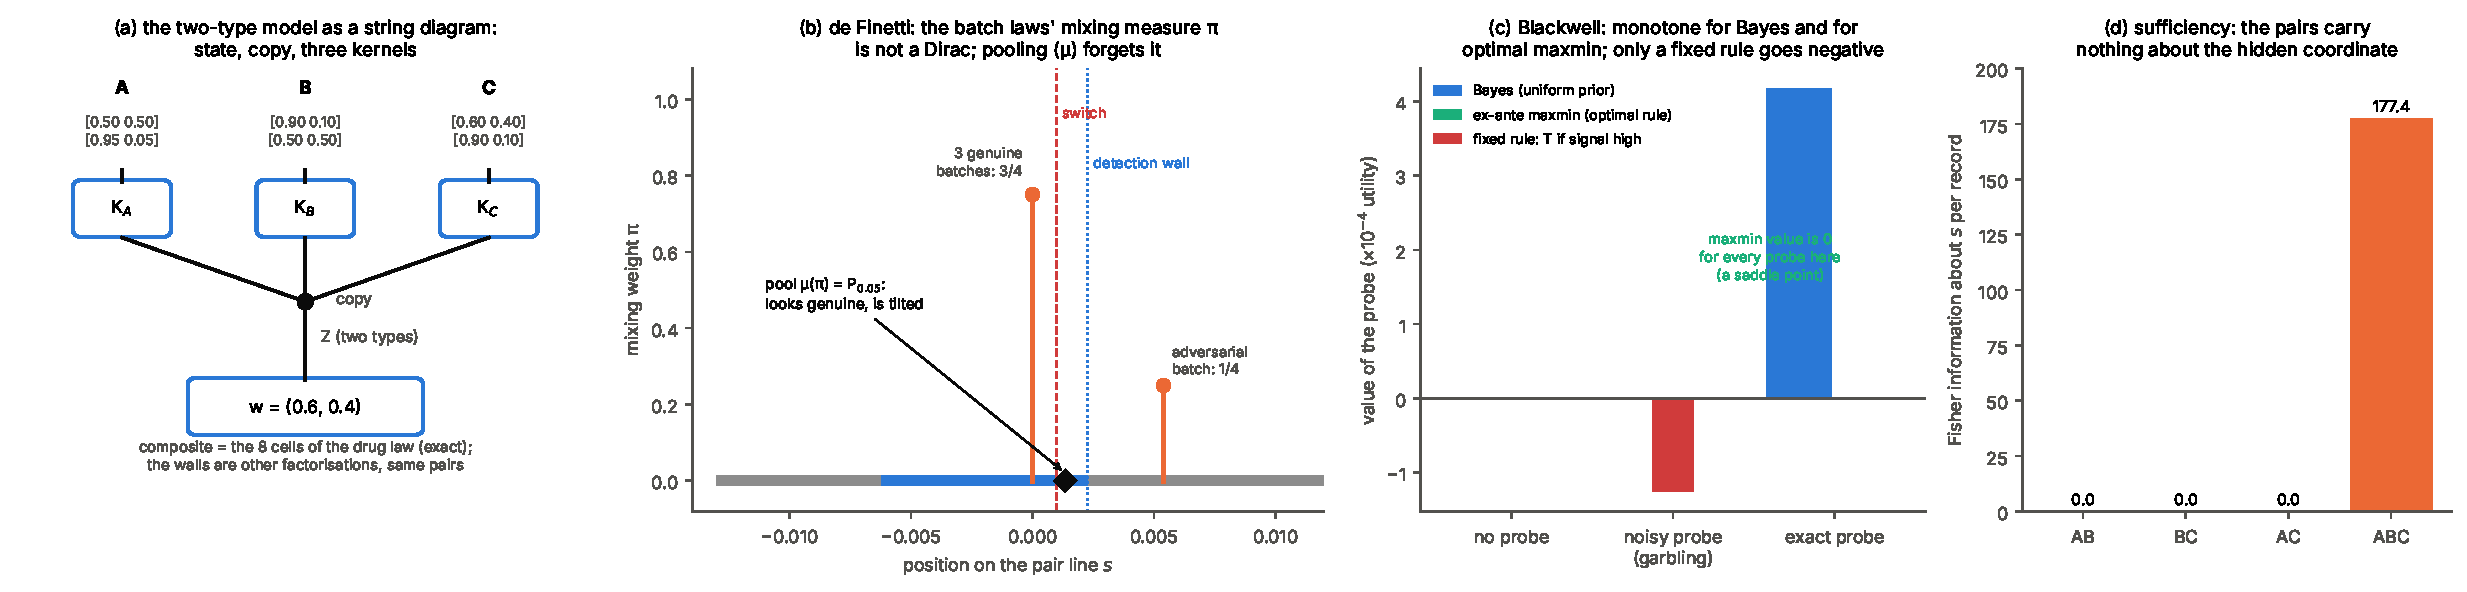
\includegraphics[width=\linewidth]{fig_markov.pdf}
\caption{Markov categories on the worked examples. (a) The two-type model as a string diagram: the state $w$, the copy map, and three
kernels (their matrices above). (b) De Finetti for four batches: the batch laws on the pair line, with their mixing weights. The pool
$\mu(\pi)$ (diamond) lands past the switch and inside the detection wall, so it is tilted and unflagged. (c) Blackwell on a
three-point slice: value of the probe for Bayes (uniform prior) and for ex-ante maxmin, for no, noisy and exact probes. Only a fixed
rule goes negative. (d) Fisher information about the hidden coordinate per record: zero in every pair window.}\label{fig:markov}
\end{figure}

\section{Assembly: descent, identification and decision}\label{sec:assembly}
The theorems of the paper answer three separate questions about observed window tables $O$: does a global law exist, does a
latent-model law exist, and how does a decision respond? The answers are not one obstruction. This section states them together, with
three separate conclusions. It is an assembly of results proved above, not a new theorem; its value is that it shows where each
conclusion comes from.

\begin{theorem}[descent, identification, decision]\label{thm:N}
Two latent types, the pair cover on three binary variables, and window tables $O$ (with source and batch labels where stated).
\begin{enumerate}
\item[(i)] \emph{Existence.} The global laws consistent with $O$ form the polytope $F(O)=(P+\ker K)\cap\Delta$, a translate of the kernel
  $\ker K=\mathbb R\chi_{ABC}$ cut by positivity. $F(O)$ is non-empty if and only if $O$ is compatible on overlaps (zero Čech energy) and
  passes the positivity programme ($\lambda^*=1$). Equivalently, $\sigma_O$ lies in the precone of Roumen's connecting map.
  Compatibility alone gives only a signed law. For labelled batches whose tables come from batch laws, a common law exists if and only if
  $\delta^0$ vanishes on every window.
  (\cref{prop:spectrum,prop:csd,prop:comonadic}; \cite{Roumen2017}, Theorem~10.5.)
\item[(ii)] \emph{Latent-model membership.} $F(O)$ contains a two-type law if and only if the sign class in $H^1(\Gamma;\mathbb Z/2)$
  vanishes and the walls leave a segment. The two-type laws in $F(O)$ then form the hiding segment, and a triple window decides whether the
  law lies on it (stage $D_5$). The label switch is the kernel of this layer.
  (\cref{thm:A}; \cref{thm:M}(1)--(5); \cref{cor:filtration}.)
\item[(iii)] \emph{Decision sensitivity.} For a decision with walls $\{\ell_j=c_j\}$:
  \begin{itemize}
  \item it is settled before a probe if and only if the hiding segment lies in one chamber;
  \item a probe's Savage value is $R(\mathcal M)-\max_yR(S_y)$, and its Wald value is positive if and only if a wall crosses the segment
    with strictly opposite slopes;
  \item every robustness number is the margin to a wall over a capacity: forward and observer injection budgets, settling size, and the
    labelled band of $B=c_s\sqrt{\pi/(1-\pi)}$ standard errors. Under labels, an unexposed source can delay the decision, by a factor of
    at most $((z+B)/z)^2$, but cannot tilt it when $B<z$.
  \end{itemize}
  (\cref{thm:D,thm:L,thm:J}; \cref{prop:voisize}.)
\end{enumerate}
\end{theorem}

\begin{proof}
Each item is the cited result restricted to the stated setting. (i) The kernel and the signed surjectivity are \cref{prop:spectrum}. The
positivity criterion is the marginal-problem linear programme, which equals Roumen's precone test by his Proposition~10.4 (check RO3). The
labelled case is \cref{prop:comonadic}(iii). (ii) \Cref{thm:M}(2), (3) and (5) and the strictness witnesses of \cref{cor:filtration}.
(iii) \Cref{thm:L}(1)--(3) and \cref{thm:J}(2)--(4).
\end{proof}

The three conclusions can fail independently. Each combination occurs in the lab:
\begin{itemize}
\item a family can glue and fail (ii): the ``exactly one harm'' law;
\item it can pass (i) and (ii) and still be decision-fragile: the drug example's margin is $0.001$, and the observer's block is $1/128$;
\item it can be tilted while passing every test: the hidden channel inside the stealth window, which only labels or a second triple
  expose.
\end{itemize}
The theorem is stated for two types, the pair cover and three variables. Parts of (i) and (iii) hold on any fibre, because they use only
linearity and positivity. Its extension to more types, where the model part is a non-convex secant variety and the label switch becomes
the symmetric group $S_k$, and to other covers, is open.

\section{Relation to the geometry, and open problems}\label{sec:open}
\Cref{thm:A} rests on the moment normal form and the Stanley--Reisner structure of the latent fibre in \cite{PG}. Its strata, where
types agree on variables or merge, are the hiding places the theorems measure.

At level one, gluing tables along observed separators is Sullivant's toric fibre product
\cite{Sullivant2007,EngstromKahleSullivant2014}. The latent model needs gluing along a hidden separator, because the type is in every
window. A rule for that case would say which covers identify the actors and would extend \cref{thm:A} beyond the pair cover. We do not
know one.

\paragraph{Related work.} Deciding over the set of parameters that the data cannot distinguish is the programme of partial
identification \cite{Manski2000,Stoye2009,GiacominiKitagawa2021,MontielOleaQiuStoye2023,Manski2025}. Identified sets of discrete models with
unobserved variables are fibres of polynomial maps, and \cite{DuarteEtAl2024} compute them by polynomial programming. That literature
treats the identified set as a generic set, often an interval. What the lab adds is the use of its algebraic structure (degree, strata,
moment factorisation) to obtain decision-theoretic results: the two wall checks, the stratified value of a probe, the settling size,
the hidden channel, and the nesting of the adversary's segment and the regulator's on one line. Singular learning theory \cite{Watanabe2009,DrtonPlummer2017} uses the same singular geometry for estimation
and model choice, not for decisions. Horowitz and Manski \cite{HorowitzManski1995} identify a distribution from contaminated data; their identified set is the
regulator's side of the reachable polytope of \cref{thm:E}(1). Part II sits in robust statistics \cite{Huber1964,Hampel1974} and the study of data poisoning
\cite{BiggioNelsonLaskov2012,SteinhardtKohLiang2017,DiakonikolasEtAl2019}.

Further open problems:
\begin{itemize}
\item decisions that combine the segment with level-one contamination, and settling for utilities on four or more variables
  (\cref{thm:D} covers the two-type pair cover and, for settling, three variables);
\item more than two types, where the segment becomes a higher-dimensional cell;
\item a real test on published aggregate trial tables;
\item injection into separate windows, which can break gluing ($\lambda^*<1$) and be caught at level one, and editing of genuine records
  (a total-variation ball);
\item an adversary uncertain about $P$, and obstructions beyond second order on the strata;
\item choosing windows to minimise the hidden channel's capacity.
\end{itemize}

\section{Scope of each result}\label{sec:scope}
Several results hold well beyond the setting in which the paper develops them, and others hold only in that setting. To prevent
misreading, \cref{tab:scope} records for each result the number of latent types, the cover and the number of variables for which it is
proved, why it extends when it does, and what is open. ``Any'' means the proof uses only linearity of expected utility in the law and
positivity, or a statement about an arbitrary graph or cover. ``Computed'' means verified for the listed cases by a check, with no
general proof.

{\small\renewcommand{\arraystretch}{1.12}
\begin{longtable}{p{0.19\linewidth}p{0.06\linewidth}p{0.15\linewidth}p{0.1\linewidth}p{0.34\linewidth}}
\caption{Scope by result. ``Types'' is the number of latent types; ``Var.''\ the number of binary variables.}\label{tab:scope}\\\toprule
result & types & cover & var. & why it extends, and what is open\\\midrule\endfirsthead
\toprule result & types & cover & var. & why it extends, and what is open\\\midrule\endhead
\multicolumn{5}{l}{\emph{Part I: the hiding segment and the decision}}\\*
A: hiding segment & 2 & pair & $m\ge3$ & needs three non-zero $v_i$. Open: $k\ge3$ (a higher-dimensional, non-convex hiding set); partial covers\\
B: tempo & 2 & pair, $+$triple & any $m$ & open: $k\ge3$; bipartite covers, where $|v|$ is not pinned\\
C: value of a probe & 2 & pair $+$ one triple & any $m$ & open: several probes jointly; other covers; $k\ge3$\\
D: decision on the segment & 2 & pair & any $m$; settling $m=3$ & settling needs affine utilities in $r$ (three variables). Open: settling for $m\ge4$\\[3pt]
\multicolumn{5}{l}{\emph{Part II: injected records}}\\*
E: slopes, vertex attack & any & any & any & linear in the injected law; exact for linear decision functionals\\
F: hidden channel & 2 & pair & $m=3$; (4) any $m$ & (4) covers one triple $S$ at any $m$. Open: several channels moved jointly\\
G: stealth with equations & 2 & pair & $m=4$ & open: $m\ge5$, where more model equations appear\\
H: one geometry & 2 & pair & $m=3$, $4$ & open: $m\ge5$\\
J: sources and bands & any & labelled, one scalar statistic & any & band formula for any scalar statistic in the Gaussian limit. Open: several statistics; adaptive adversaries over rounds\\
Study 13 & 2 & pair $+$ triple, 3 sources & 3 & one registered truth\\[3pt]
\multicolumn{5}{l}{\emph{Lifting and the one picture}}\\*
K(1), (2), (4) & any & any & any & linear in the law; act lift by the minimax theorem\\
K(3): blow-up of the merge & 2 & pair & any $m$ & open: blow-ups for $k\ge3$\\
K(5): orbifold atlas & 2 & pair & $m=4$ & standard toric geometry; the Markov-basis reading is conjectural\\
L(3), (4): margin over capacity, relevance & any & any fibre & any & support function of the gauge; linearity\\
L(1), (2), (5) & 2 & pair & $m=3$ & open: $m\ge4$, where the model part is a curve in a higher-dimensional fibre\\
dilation; value in probe size; backtracking & 2 & pair & $m=3$ & worked example; dilation width $\Delta s/P(a,b)$ holds on any pair line\\
price of not gluing (rectangularity) & --- & finite trees & --- & proved; sharpness conjectural\\[3pt]
\multicolumn{5}{l}{\emph{Descent and categorical structure}}\\*
spectrum and descent & any & any cover & any & kernel and signed surjectivity in general; acyclicity computed for the pair covers ($m=3,4$) and the triple cover ($m=4$)\\
M(1)--(3): sign and modulus classes & 2 & any graph of pairs & any & $H^1(\Gamma;\mathbb Z/2)\oplus\operatorname{coker}B$ for any graph. Open: $S_k$ coefficients for $k\ge3$ (non-abelian)\\
M(4), (5): triple layer, fibre & 2 & triple cover; pair & $m=4$; $m=3$ & open: $m\ge5$\\
M(6), (7): labels; realization diagram & any; 2 & labelled; pair & any & degree-$0$ statement for any labelled cover\\
descent filtration (corollary) & 2 & any connected pair graph & any & strictness witnesses computed at $m=3,4$; the counts $E-\operatorname{rank}B$ and $b_1$ are general\\
comonadic form & any & any cover & any & classical theorems; the lab uses their object-level consequences\\
CSD no-go & any & covers with a cycle & any & counterexamples on the triangle; degrees computed for the pair covers\\
quantum marginal problem & --- & qubit windows & any & dephasing retraction general; the kernel count ($27$) is for three qubits\\
Markov categories & any & any & any & factorisation for $k$ types is a $k$-point object; Blackwell and de Finetti as cited\\
Ring of contingency tables (\cref{sec:ehrhart}) & 2 & pair & $m=3$ & fibre and Gr\"obner statements hold for any table model; the hiding set, $\tau_c$ and Study 11c are for three binary variables\\
Tangent structure \cite{TangentCompanion} & any & polyhedra & any & cone structure on any polyhedron with affine maps; universality iff relative interior; jets proved on the $m=4$ tetrad scheme\\
Roumen's order cohomology & any & any & any & his Theorem~10.5; equals the marginal-problem LP\\
N: assembly & 2 & pair & $m=3$ & as its parts\\\bottomrule
\end{longtable}}

The pattern is consistent. Results that rest on linearity and positivity hold on any fibre and any cover. These are the slopes, margin
over capacity, the relevance criterion, the source band, the descent kernel and the positivity criterion. Results that rest on the
geometry of the two-type model need its parametrisation. These are the hiding segment, the tempos, settling, the closed forms of the
hidden channel, and realizability. They are proved for two types, mostly on the pair cover, and some only for three or four variables.
Two companion projects take up the narrow results. One builds the tangent structure \cite{TangentCompanion}; it is now written. The other develops the
two-type theory on arbitrary covers, with a three-type computation as a proof of concept for $S_k$ descent.

\section{Limits}
\begin{itemize}
\item All data are synthetic.
\item Part II treats whole-record injection by an adversary who knows $P$; the hidden channel is for $m=3$ and the detection test for
  $m=4$ uses only the tetrads.
\item There are two types and binary variables.
\item Theorem D's settling part covers utilities on three variables; Study 11b tests it on five designs and two truths.
\item The decision in Study 11 is one stylised treatment choice. Its Wald gap $g$ is $0$ by a saddle point; the regret illustration uses a
  post-hoc cost.
\item The disclosure game assumes the sponsor knows the truth.
\item The regulator's naive policy uses the segment's midpoint.
\item The illustrations are stylised.
\item In Study 11, three registered predictions and one illustration failed, as reported.
\item The settling predictions use the delta method and the plug-in $\hat\tau$; they were tested from $n^*/2$ upward, not at small $n$.
  Study 11c's exact probe assumes the pair tables are known.
\end{itemize}

\appendix
\section{Reproducibility}
{\raggedright
\begin{itemize}
\item \texttt{engine/pce/lab.py} implements the model, the segment and sampling.
\item Study 11 is in \texttt{engine/study11\_lab/}:
  \begin{itemize}
  \item the registration and its hash manifest: \texttt{PREREG\_study11.md}, \texttt{FROZEN\_PREREG\_study11.txt};
  \item the frozen script as a text copy: \texttt{run\_study11\_as\_frozen.py.txt};
  \item the script that was run, with the logged deviation: \texttt{run\_study11.py}, \texttt{DEVIATIONS\_study11.md};
  \item results and post-hoc analyses: \texttt{results\_study11.json}, \texttt{posthoc\_study11.py}, \texttt{posthoc\_study11.json} (PH1--PH4).
  \end{itemize}
\item \texttt{engine/pce/segment\_decision.py} implements \cref{thm:D}: the utility polynomials, the set and info-gap rules, the
  settling constraints and the $m=3$ estimator; \texttt{engine/check\_decision\_segment.py} runs checks DS1--DS9.
\item Study 11b is in \texttt{engine/study11b\_settle/}: \texttt{PREREG\_study11b.md}, \texttt{FROZEN\_PREREG\_study11b.txt},
  \texttt{design11b.py}, \texttt{run\_study11b.py} (with a frozen text copy), \texttt{results\_study11b.json}.
\item Study 11c is in \texttt{engine/study11c\_exact/}: \texttt{PREREG\_study11c.md}, \texttt{FROZEN\_PREREG\_study11c.txt},
  \texttt{run\_study11c.py} (with a frozen text copy), \texttt{results\_study11c.json}; the ring-of-tables checks are
  \texttt{engine/check\_ehrhart.py} (EH1--EH7) with \texttt{engine/pce/ehrhart.py}, and the figure is \texttt{lab/fig\_ehrhart.py}.
\item \texttt{engine/pce/injection.py} implements Part II: the injected law, the hidden channel, influence functions, budgets, the
  tetrads and the stealth--tilt programme; \texttt{engine/pce/duality.py} implements \cref{thm:H} and the obstruction of
  \cref{thm:G}(4); \texttt{engine/check\_injection.py} runs checks IN1--IN14.
\item Study 12 is in \texttt{engine/study12\_inject/}: \texttt{PREREG\_study12.md}, \texttt{FROZEN\_PREREG\_study12.txt},
  \texttt{design12.py}, \texttt{run\_study12.py} (with a frozen text copy), \texttt{results\_study12.json}.
\item \texttt{engine/worked\_example.py} recomputes every number of \cref{sec:example} and checks it (WE0--WE18), writing
  \texttt{lab/worked\_example.json}.
\item \texttt{engine/worked\_example4.py} recomputes the four-variable example of \cref{sec:example4} in stages and checks it
  (W4-1 to W4-14), writing \texttt{lab/worked\_example4.json}.
\item \texttt{lab/fig\_lab.py} draws every figure.
\item The pairwise proposition is check SC7 of \cite{PG}.
\end{itemize}\par}

\begin{thebibliography}{99}\small
\bibitem{Coupling} V.~K. Awasthi, Coupling polytopes and toric geometry: the $2\times3$ family, the square case, higher levels and stability, technical report, October 2026 (revised).

\bibitem{Delzant1988} T.~Delzant, Hamiltoniens périodiques et images convexes de l'application moment, \emph{Bull. Soc. Math. France} \textbf{116} (1988) 315--339.

\bibitem{PachterSturmfels2005} L.~Pachter and B.~Sturmfels (eds.), \emph{Algebraic Statistics for Computational Biology}, Cambridge University Press, 2005.

\bibitem{GelfandKapranovZelevinsky1994} I.~M.~Gelfand, M.~M.~Kapranov and A.~V.~Zelevinsky, \emph{Discriminants, Resultants, and Multidimensional Determinants}, Birkhäuser, 1994.

\bibitem{ChoOh2006} C.-H.~Cho and Y.-G.~Oh, Floer cohomology and disc instantons of Lagrangian torus fibers in Fano toric manifolds, \emph{Asian J. Math.} \textbf{10} (2006) 773--814.

\bibitem{LermanTolman1997} E.~Lerman and S.~Tolman, Hamiltonian torus actions on symplectic orbifolds and toric varieties, \emph{Trans. Amer. Math. Soc.} \textbf{349} (1997) 4201--4230.

\bibitem{TowerGeometry} V.~K. Awasthi, Shadows, fibres and secants of the posterior tower, technical report, October 2026.

\bibitem{PG} V.~K. Awasthi, Partial gluing and level two: graded explanations, latent actors and paths through singularities, technical note, October 2026.
\bibitem{Boyd} J.~R. Boyd, \emph{A Discourse on Winning and Losing}, briefing (1987); Air University Press edition, 2018.
\bibitem{Knight1921} F.~H. Knight, \emph{Risk, Uncertainty and Profit}, Houghton Mifflin, 1921.
\bibitem{Wald1950} A.~Wald, \emph{Statistical Decision Functions}, Wiley, 1950.
\bibitem{GilboaSchmeidler1989} I.~Gilboa and D.~Schmeidler, Maxmin expected utility with non-unique prior, \emph{J. Math. Econ.} \textbf{18} (1989) 141--153.
\bibitem{BenHaim2006} Y.~Ben-Haim, \emph{Info-Gap Decision Theory}, 2nd ed., Academic Press, 2006.
\bibitem{SchwartzBenHaimDacso2011} B.~Schwartz, Y.~Ben-Haim and C.~Dacso, What makes a good decision? Robust satisficing as a normative standard of rational decision making, \emph{J. Theory Soc. Behav.} \textbf{41} (2011) 209--227.
\bibitem{LongSimZhou2023} D.~Z. Long, M.~Sim and M.~Zhou, Robust satisficing, \emph{Oper. Res.} \textbf{71} (2023) 61--82.
\bibitem{Howard1966} R.~A. Howard, Information value theory, \emph{IEEE Trans. Syst. Sci. Cybern.} \textbf{2} (1966) 22--26.
\bibitem{Blackwell1953} D.~Blackwell, Equivalent comparisons of experiments, \emph{Ann. Math. Statist.} \textbf{24} (1953) 265--272.
\bibitem{AlNajjarWeinstein2009} N.~I. Al-Najjar and J.~Weinstein, The ambiguity aversion literature: a critical assessment, \emph{Econ. Philos.} \textbf{25} (2009) 249--284.
\bibitem{Savage1951} L.~J.~Savage, The theory of statistical decision, \emph{J. Amer. Statist. Assoc.} \textbf{46} (1951) 55--67.

\bibitem{Siniscalchi2011} M.~Siniscalchi, Dynamic choice under ambiguity, \emph{Theor. Econ.} \textbf{6} (2011) 379--421.
\bibitem{KamenicaGentzkow2011} E.~Kamenica and M.~Gentzkow, Bayesian persuasion, \emph{Amer. Econ. Rev.} \textbf{101} (2011) 2590--2615.
\bibitem{Milgrom1981} P.~R. Milgrom, Good news and bad news: representation theorems and applications, \emph{Bell J. Econ.} \textbf{12} (1981) 380--391.
\bibitem{Grossman1981} S.~J. Grossman, The informational role of warranties and private disclosure about product quality, \emph{J. Law Econ.} \textbf{24} (1981) 461--483.
\bibitem{HenryOttaviani2019} E.~Henry and M.~Ottaviani, Research and the approval process: the organization of persuasion, \emph{Amer. Econ. Rev.} \textbf{109} (2019) 911--955.
\bibitem{DiTillioOttavianiSorensen2021} A.~Di~Tillio, M.~Ottaviani and P.~N. Sørensen, Strategic sample selection, \emph{Econometrica} \textbf{89} (2021) 911--953.
\bibitem{Chen1995} J.~Chen, Optimal rate of convergence for finite mixture models, \emph{Ann. Statist.} \textbf{23} (1995) 221--233.
\bibitem{KaelblingLittmanCassandra1998} L.~P. Kaelbling, M.~L. Littman and A.~R. Cassandra, Planning and acting in partially observable stochastic domains, \emph{Artif. Intell.} \textbf{101} (1998) 99--134.
\bibitem{Lindley1956} D.~V. Lindley, On a measure of the information provided by an experiment, \emph{Ann. Math. Statist.} \textbf{27} (1956) 986--1005.
\bibitem{ChalonerVerdinelli1995} K.~Chaloner and I.~Verdinelli, Bayesian experimental design: a review, \emph{Statist. Sci.} \textbf{10} (1995) 273--304.
\bibitem{ShiLiangShroff2023} M.~Shi, Y.~Liang and N.~B.~Shroff, Near-optimal partially observable reinforcement learning with partial online state information, arXiv:2306.08762v4 (first version 2023, titled ``Theoretical hardness and tractability of POMDPs in RL with partial online state information''; a preliminary version appeared at IEEE MILCOM 2024).

\bibitem{ShenDongHuan2023} W.~Shen, J.~Dong and X.~Huan, Variational sequential optimal experimental design using reinforcement learning, arXiv:2306.10430 (2023).
\bibitem{Goodfellow2014} I.~Goodfellow et al., Generative adversarial nets, \emph{Advances in Neural Information Processing Systems} \textbf{27} (2014).
\bibitem{Mescheder2018} L.~Mescheder, A.~Geiger and S.~Nowozin, Which training methods for GANs do actually converge?, \emph{Proc. ICML}, PMLR \textbf{80} (2018).
\bibitem{Nowozin2016} S.~Nowozin, B.~Cseke and R.~Tomioka, $f$-GAN: training generative neural samplers using variational divergence minimization, \emph{Advances in Neural Information Processing Systems} \textbf{29} (2016).
\bibitem{Sullivant2007} S.~Sullivant, Toric fiber products, \emph{J. Algebra} \textbf{316} (2007) 560--577.
\bibitem{EngstromKahleSullivant2014} A.~Engström, T.~Kahle and S.~Sullivant, Multigraded commutative algebra of graph decompositions, \emph{J. Algebraic Combin.} \textbf{39} (2014) 335--372.
\bibitem{Quillen1970} D.~Quillen, On the (co-)homology of commutative rings, in \emph{Applications of Categorical Algebra}, Proc. Sympos. Pure Math. \textbf{17}, Amer. Math. Soc., 1970, 65--87.

\bibitem{Andre1974} M.~André, \emph{Homologie des algèbres commutatives}, Springer, 1974.

\bibitem{HorowitzManski1995} J.~L.~Horowitz and C.~F.~Manski, Identification and robustness with contaminated and corrupted data, \emph{Econometrica} \textbf{63} (1995) 281--302.

\bibitem{BlanchardEtAl2017} P.~Blanchard, E.~M.~El~Mhamdi, R.~Guerraoui and J.~Stainer, Machine learning with adversaries: Byzantine tolerant gradient descent, \emph{NeurIPS} (2017).
\bibitem{BaruchEtAl2019} M.~Baruch, G.~Baruch and Y.~Goldberg, A little is enough: circumventing defenses for distributed learning, \emph{NeurIPS} (2019).
\bibitem{YinEtAl2018} D.~Yin, Y.~Chen, K.~Ramchandran and P.~Bartlett, Byzantine-robust distributed learning: towards optimal statistical rates, \emph{ICML} (2018).
\bibitem{SeidenfeldWasserman1993} T.~Seidenfeld and L.~Wasserman, Dilation for sets of probabilities, \emph{Ann. Statist.} \textbf{21} (1993) 1139--1154.
\bibitem{RadnerStiglitz1984} R.~Radner and J.~E.~Stiglitz, A nonconcavity in the value of information, in M.~Boyer and R.~Kihlstrom (eds.), \emph{Bayesian Models in Economic Theory}, North-Holland (1984) 33--52.
\bibitem{EpsteinSchneider2003} L.~G.~Epstein and M.~Schneider, Recursive multiple-priors, \emph{J. Econ. Theory} \textbf{113} (2003) 1--31.
\bibitem{FournierFacioWillett2026} F.~Fournier-Facio and R.~Willett, The local lifting property, property FD, and stability of approximate representations, arXiv:2603.18456 (2026).
\bibitem{Li2026} G.~Li, Derived representation schemes with arbitrary coefficients and associative smoothness, arXiv:2607.19654 (2026).
\bibitem{AbramskyBrandenburger2011} S.~Abramsky and A.~Brandenburger, The sheaf-theoretic structure of non-locality and contextuality, \emph{New J. Phys.} \textbf{13} (2011) 113036.
\bibitem{ChangCSD2026} S.-Y.~Chang, Universal obstruction cohomology of categorified spectral objects: from descent filtrations to derived duality, preprint hal-05711275 (2026).
\bibitem{AbramskyMansfieldBarbosa2012} S.~Abramsky, S.~Mansfield and R.~S.~Barbosa, The cohomology of non-locality and contextuality, \emph{EPTCS} \textbf{95} (2012) 1--14.
\bibitem{BenabouRoubaud1970} J.~Bénabou and J.~Roubaud, Monades et descente, \emph{C. R. Acad. Sci. Paris Sér. A} \textbf{270} (1970) 96--98.
\bibitem{Beck1967} J.~M.~Beck, \emph{Triples, Algebras and Cohomology}, PhD thesis, Columbia University (1967); Reprints in Theory Appl. Categ. \textbf{2} (2003).
\bibitem{JanelidzeTholen1994} G.~Janelidze and W.~Tholen, Facets of descent, I, \emph{Appl. Categ. Structures} \textbf{2} (1994) 245--281.
\bibitem{EilenbergMoore1965} S.~Eilenberg and J.~C.~Moore, Adjoint functors and triples, \emph{Illinois J. Math.} \textbf{9} (1965) 381--398.
\bibitem{MacLane1998} S.~Mac~Lane, \emph{Categories for the Working Mathematician}, 2nd ed., Springer (1998).
\bibitem{Godement1958} R.~Godement, \emph{Topologie algébrique et théorie des faisceaux}, Hermann, Paris (1958).
\bibitem{Weibel1994} C.~A.~Weibel, \emph{An Introduction to Homological Algebra}, Cambridge University Press (1994).
\bibitem{Giraud1971} J.~Giraud, \emph{Cohomologie non abélienne}, Springer (1971).
\bibitem{Giry1982} M.~Giry, A categorical approach to probability theory, in \emph{Categorical Aspects of Topology and Analysis}, Lecture Notes in Math. \textbf{915}, Springer (1982) 68--85.
\bibitem{Ikeda2025} K.~Ikeda, Quantum entanglement as a cohomological obstruction, arXiv:2511.04326v2 (2026).
\bibitem{Fritz2020} T.~Fritz, A synthetic approach to Markov kernels, conditional independence and theorems on sufficient statistics, \emph{Adv. Math.} \textbf{370} (2020) 107239.
\bibitem{FritzGondaPerrone2021} T.~Fritz, T.~Gonda and P.~Perrone, De Finetti's theorem in categorical probability, \emph{J. Stoch. Anal.} \textbf{2}(4) (2021), Article 6; arXiv:2105.02639.
\bibitem{ChenEtAl2025} L.~Chen, T.~Fritz, T.~Gonda, A.~Klingler and A.~Lorenzin, The Aldous--Hoover theorem in categorical probability, \emph{Algebr. Stat.} \textbf{16} (2025) 131--174; arXiv:2411.12840.
\bibitem{FritzGondaPerroneRischel2023} T.~Fritz, T.~Gonda, P.~Perrone and E.~F.~Rischel, Representable Markov categories and comparison of statistical experiments in categorical probability, arXiv:2010.07416.
\bibitem{CouplingAlgebras} V.~K.~Awasthi, Coupling algebras: gluing, the square-zero cone and the ring of contingency tables, technical report, Johns Hopkins University, October 2026, draft 4.
\bibitem{TangentCompanion} V.~K.~Awasthi, A tangent structure for injected data: feasible cones, universality at corners, and jets on the tetrad scheme, companion paper, 2026.
\bibitem{CockettCruttwell2014} J.~R.~B.~Cockett and G.~S.~H.~Cruttwell, Differential structure, tangent structure, and SDG, \emph{Appl. Categ. Structures} \textbf{22} (2014) 331--417.
\bibitem{Roumen2017} F.~Roumen, Cohomology of effect algebras, \emph{EPTCS} \textbf{236} (2017) 174--201; arXiv:1602.00567.
\bibitem{YinZhang2022} Y.~Yin and J.~Zhang, Markov categories, causal theories, and the do-calculus, \emph{Studies in Logic} (2021); arXiv:2204.04821.
\bibitem{DiLavoreRomanSobocinski2025} E.~Di~Lavore, M.~Román and P.~Sobociński, Partial Markov categories, arXiv:2502.03477 (2025).
\bibitem{Manski2025} C.~F.~Manski, Identification and statistical decision theory, \emph{Econometric Theory} \textbf{41}(4) (2025) 977--993; arXiv:2204.11318.
\bibitem{Huber1964} P.~J.~Huber, Robust estimation of a location parameter, \emph{Ann. Math. Statist.} \textbf{35} (1964) 73--101.

\bibitem{Hampel1974} F.~R.~Hampel, The influence curve and its role in robust estimation, \emph{J. Amer. Statist. Assoc.} \textbf{69} (1974) 383--393.

\bibitem{BiggioNelsonLaskov2012} B.~Biggio, B.~Nelson and P.~Laskov, Poisoning attacks against support vector machines, \emph{Proc. ICML} (2012), arXiv:1206.6389.

\bibitem{SteinhardtKohLiang2017} J.~Steinhardt, P.~W.~Koh and P.~Liang, Certified defenses for data poisoning attacks, \emph{Advances in Neural Information Processing Systems} \textbf{30} (2017), arXiv:1706.03691.

\bibitem{DiakonikolasEtAl2019} I.~Diakonikolas, G.~Kamath, D.~Kane, J.~Li, A.~Moitra and A.~Stewart, Robust estimators in high dimensions without the computational intractability, \emph{SIAM J. Comput.} \textbf{48} (2019) 742--864.

\bibitem{DrtonSturmfelsSullivant2007} M.~Drton, B.~Sturmfels and S.~Sullivant, Algebraic factor analysis: tetrads, pentads and beyond, \emph{Probab. Theory Related Fields} \textbf{138} (2007) 463--493, doi:10.1007/s00440-006-0033-2.

\bibitem{Manski2000} C.~F.~Manski, Identification problems and decisions under ambiguity: empirical analysis of treatment response and normative analysis of treatment choice, \emph{J. Econometrics} \textbf{95} (2000) 415--442.

\bibitem{Stoye2009} J.~Stoye, Minimax regret treatment choice with finite samples, \emph{J. Econometrics} \textbf{151} (2009) 70--81.

\bibitem{GiacominiKitagawa2021} R.~Giacomini and T.~Kitagawa, Robust Bayesian inference for set-identified models, \emph{Econometrica} \textbf{89} (2021) 1519--1556.

\bibitem{MontielOleaQiuStoye2023} J.~L.~Montiel Olea, C.~Qiu and J.~Stoye, Decision theory for treatment choice problems with partial identification, arXiv:2312.17623.

\bibitem{DuarteEtAl2024} G.~Duarte, N.~Finkelstein, D.~Knox, J.~Mummolo and I.~Shpitser, An automated approach to causal inference in discrete settings, \emph{J. Amer. Statist. Assoc.} \textbf{119} (2024) 1778--1793.

\bibitem{Watanabe2009} S.~Watanabe, \emph{Algebraic Geometry and Statistical Learning Theory}, Cambridge University Press, 2009.

\bibitem{DrtonPlummer2017} M.~Drton and M.~Plummer, A Bayesian information criterion for singular models, \emph{J. R. Stat. Soc. Ser. B} \textbf{79} (2017) 323--380.

\end{thebibliography}
\end{document}
